\documentclass[12pt]{extarticle}
\usepackage[utf8]{inputenc}
\usepackage[main=spanish, english]{babel}
\usepackage{csquotes}
\usepackage{graphicx}
\usepackage{fancyhdr}
\usepackage{geometry}
\usepackage{lipsum}
\usepackage{tocloft} 
\usepackage{amsmath}
\numberwithin{equation}{section}
\setlength{\jot}{14pt}
\usepackage{amssymb}
\usepackage{float}
\usepackage{caption}
\usepackage{pifont}
\usepackage[table,xcdraw]{xcolor}
\usepackage{algpseudocode}
\usepackage{algorithm}
\usepackage{booktabs}
\usepackage{multirow}
\usepackage{listings}
\usepackage{subfiles}
\usepackage{tikz}
\usetikzlibrary{positioning, arrows.meta, shapes.geometric, fit, backgrounds}

\lstset{
  language=Python,
  basicstyle=\ttfamily\scriptsize,
  keywordstyle=\color{blue},
  stringstyle=\color{teal},
  commentstyle=\color{gray}\itshape,
  numbers=left,
  numberstyle=\tiny,
  frame=none,
  captionpos=b,
  breaklines=true,
  showstringspaces=false
}

\definecolor{darkred}{rgb}{0,0,0}
\definecolor{darkgreen}{rgb}{0,0.8,0}
\definecolor{darkblue}{rgb}{0,0,1}

\usepackage[
    backend=biber,
    style=ieee
]{biblatex}

\addbibresource{ref_tfg.bib}
\addbibresource{ref_executive_summary.bib}

\usepackage{hyperref}
\hypersetup{
    colorlinks,
    linkcolor=darkred,
    filecolor=darkblue,
    urlcolor=darkred,
    citecolor=darkgreen
}

% Language-dependent names
\addto\captionsspanish{
    \renewcommand{\contentsname}{Índice}
    \renewcommand{\listfigurename}{Índice de figuras}
    \renewcommand{\listtablename}{Índice de tablas}
    \renewcommand{\figurename}{Figura}
    \renewcommand{\tablename}{Tabla}
    \renewcommand{\lstlistingname}{Algoritmo}
    \floatname{algorithm}{Algoritmo}
}

\addto\captionsenglish{
    \renewcommand{\contentsname}{Contents}
    \renewcommand{\listfigurename}{List of Figures}
    \renewcommand{\listtablename}{List of Tables}
    \renewcommand{\figurename}{Figure}
    \renewcommand{\tablename}{Table}
    \renewcommand{\lstlistingname}{Algorithm}
    \floatname{algorithm}{Algorithm}
}

% Language-dependent autoref names
\addto\extrasspanish{
    \renewcommand{\tableautorefname}{Tabla}
    \renewcommand{\figureautorefname}{Figura}
    \renewcommand{\equationautorefname}{Ecuación}
    \renewcommand{\sectionautorefname}{Sección}
    \renewcommand{\subsectionautorefname}{Sección}
}

\addto\extrasenglish{
    \renewcommand{\tableautorefname}{Table}
    \renewcommand{\figureautorefname}{Figure}
    \renewcommand{\equationautorefname}{Equation}
    \renewcommand{\sectionautorefname}{Section}
    \renewcommand{\subsectionautorefname}{Section}
}

\newcommand{\blankpage}{
    \clearpage
    \thispagestyle{empty}
    \mbox{}
    \clearpage
}

\usepackage{titlesec}
\usepackage{tocloft}

\titleformat{\section}
  {\normalfont\Large\bfseries}
  {Capítulo \thesection}
  {1em}
  {}

\renewcommand{\cftsecpresnum}{Capítulo~}
\setlength{\cftsecnumwidth}{6em}



%%%%%%%%%%%%%%%%%%%%%%%%%%%%%%%%%%%%%%%%%%%%%%%%%%%%%%%%%%%%%%%%%%%%%%%%%%%%%%%%%%%%%%%%%%%
%%%%%%%%%%%%%%%%%%%%%%%%%%%%%%%%%%%%%%%%%%%%%%%%%%%%%%%%%%%%%%%%%%%%%%%%%%%%%%%%%%%%%%%%%%%
%% CONFIGURATION
%%%%%%%%%%%%%%%%%%%%%%%%%%%%%%%%%%%%%%%%%%%%%%%%%%%%%%%%%%%%%%%%%%%%%%%%%%%%%%%%%%%%%%%%%%%
%%%%%%%%%%%%%%%%%%%%%%%%%%%%%%%%%%%%%%%%%%%%%%%%%%%%%%%%%%%%%%%%%%%%%%%%%%%%%%%%%%%%%%%%%%%

\newcommand{\projectTitle}{Sistema basado en Inteligencia Artificial para el an\'alisis de texturas musculares en pacientes con enfermedades neurodegenerativas (ELA) a partir de biomarcadores ecogr\'aficos}
\newcommand{\projectTitleEnglish}{Artificial Intelligence-based System for Muscle Texture Analysis in Patients with Neurodegenerative Diseases (ALS) from Ultrasound Biomarkers}
\newcommand{\Author}{Jos\'e Juan Cortina Galindo}
\newcommand{\Director}{Constantino Malag\'on Luque}
\newcommand{\CoDirector}{}
\newcommand{\MonthToSubmit}{Junio }
\newcommand{\BeginYear}{2025}
\newcommand{\EndYear}{\number\numexpr\BeginYear+1\relax }

% Title page command
\newcommand{\ComillasTitlePage}{
\begin{titlepage}
    \centering

    
\includegraphics[width=0.35\textwidth]{images/Logo_comillas.png}\\[1cm] 

    {\Huge \textbf{GRADO EN INGENIER\'IA}}\\[0.3cm]
    {\Huge \textbf{MATEM\'ATICA E INTELIGENCIA}}\\[0.5cm]
    {\Huge \textbf{ARTIFICIAL}}\\[1.5cm]

    {\Huge \textbf{TRABAJO FIN DE GRADO}}\\[1.3cm]

    {\huge \projectTitle}\\[0.5cm]

    \vspace{20mm}

    \textbf{Autor: \Author}\\[1.0cm]
    \textbf{Director: \Director}\\

    \raisebox{-2cm}[0cm][0cm]{\large Madrid, \MonthToSubmit \EndYear}

    \vfill
\end{titlepage}
}

\newcommand{\sectionnotoc}[1]{%
    \refstepcounter{section}%
    \section*{\thesection\quad #1}%
}

\newcommand{\resetcounters}{
    \setcounter{section}{0}
    \setcounter{subsection}{0}
    \setcounter{subsubsection}{0}
    \setcounter{figure}{0}
    \setcounter{table}{0}
    \setcounter{equation}{0}
    \setcounter{footnote}{0}
}

\renewcommand{\sectionmark}[1]{%
    \markright{#1}%
}

%%%%%%%%%%%%%%%%%%%%%%%%%%%%%%%%%%%%%%%%%%%%%%%%%%%%%%%%%%%%%%%%%%%%%%%%%%%%%%%%%%%%%%%%%%%
%%%%%%%%%%%%%%%%%%%%%%%%%%%%%%%%%%%%%%%%%%%%%%%%%%%%%%%%%%%%%%%%%%%%%%%%%%%%%%%%%%%%%%%%%%%

\geometry{top=4cm, bottom=4cm, left=2.5cm, right=2.5cm}

% Margen de holgura para evitar líneas que se salgan del margen (overfull hbox)
% con palabras largas en monoespaciado (p. ej. nombres de funciones y ficheros).
\emergencystretch=3em

\begin{document}

\selectlanguage{spanish}

\ComillasTitlePage

\setlength{\headheight}{2.5cm}
\setlength{\headsep}{0.8cm}

% Configuraci\'on del encabezado
\pagestyle{fancy}
\fancyhf{}

\fancyhead[L]{
\includegraphics[width=2cm]{images/Color_logo_comillas.png}} 

\fancyhead[C]{
    \textbf{UNIVERSIDAD PONTIFICIA COMILLAS}\\
    Escuela T\'ecnica Superior de Ingenier\'ia (ICAI)\\
    Grado en Ingenier\'ia Matem\'atica e Inteligencia Artificial\\
    \small\nouppercase{\rightmark}
}

\fancyhead[R]{}

\fancyfoot[C]{\thepage}

\blankpage

\subfile{Anexo_I.tex}

\newpage

\ComillasTitlePage

\blankpage

{\fontsize{17}{20}\selectfont
    \begin{center}
        {\large Agradecimientos}
    \end{center}
    Esta sección es opcional
}

\newpage

%%%%%%%%%%%%%%%%%%%%%%%%%%%%%%%%%%%%%%%%%%%%%%%%%%%%%%%%%%%%%%%%%%%%%%%%%%%%%%%%%%%%%%%%%%%
%% RESUMEN EJECUTIVO IN SPANISH
%%%%%%%%%%%%%%%%%%%%%%%%%%%%%%%%%%%%%%%%%%%%%%%%%%%%%%%%%%%%%%%%%%%%%%%%%%%%%%%%%%%%%%%%%%%

\captionsetup[figure]{list=false}
\captionsetup[table]{list=false}

\begin{otherlanguage}{spanish}

{\large \MakeUppercase{\projectTitle}}
\vspace{3mm}

\textbf{Autor: \Author}

Director: \Director

\vspace{2mm}
Entidad colaboradora: Fundaci\'on San Juan de Dios -- ICAI, Universidad Pontificia Comillas

\begin{refsection}[ref_executive_summary.bib]

\section*{Resumen}
La Esclerosis Lateral Amiotr\'ofica (ELA) carece de un biomarcador diagn\'ostico precoz accesible. Este trabajo desarrolla un sistema de aprendizaje profundo que detecta ELA a partir de ecograf\'ia muscular, integrando cuatro grupos musculares en una decisi\'on a nivel paciente. Sobre 52 pacientes, el sistema alcanza un AUC del 98{,}67\,\%, sensibilidad del 100\,\% y especificidad del 92{,}31\,\%, a la altura de la l\'inea base cl\'inica basada en an\'alisis textural cl\'asico.

\textbf{Palabras clave}: Esclerosis Lateral Amiotr\'ofica; ecograf\'ia muscular; aprendizaje profundo; redes neuronales convolucionales; fusi\'on a nivel paciente; validaci\'on cruzada por sujeto.

\section*{Resumen ejecutivo}

\sectionnotoc{Introducci\'on}

La Esclerosis Lateral Amiotr\'ofica (ELA) es una enfermedad neurodegenerativa de pron\'ostico fatal en la que el diagn\'ostico precoz sigue siendo un reto cl\'inico: el retraso medio entre los primeros s\'intomas y el diagn\'ostico definitivo se sit\'ua en torno a los doce meses~\cite{hardiman2017als}. La ecograf\'ia muscular cuantitativa se ha propuesto como biomarcador no invasivo y de bajo coste~\cite{pillen2008muscle}, pero su interpretaci\'on requiere experiencia y los m\'etodos cl\'asicos, basados en caracter\'isticas texturales calculadas manualmente, presentan limitaciones de generalizaci\'on~\cite{martinezpaya2017quantitative}. Este Trabajo Fin de Grado aborda la automatizaci\'on del an\'alisis de texturas musculares mediante aprendizaje profundo~\cite{litjens2017survey}, integrando los cuatro grupos musculares cl\'asicamente explorados (b\'iceps, antebrazo, cu\'adriceps y tibial) en una \'unica decisi\'on diagn\'ostica formulada a nivel de paciente.

\sectionnotoc{Objetivos}

El objetivo principal es dise\~nar y validar un sistema de soporte al diagn\'ostico de ELA basado en redes neuronales convolucionales sobre ecograf\'ia muscular, operando a nivel de paciente. Como objetivos espec\'ificos: entrenar y comparar cinco arquitecturas pre-entrenadas; garantizar una validaci\'on metodol\'ogicamente honesta mediante validaci\'on cruzada estratificada y agrupada por sujeto; cuantificar la incertidumbre mediante an\'alisis estad\'istico inferencial; dise\~nar una estrategia de fusi\'on multi-m\'usculo a nivel paciente; interpretar las decisiones del modelo mediante mapas de explicabilidad; y comparar el rendimiento global frente a la l\'inea base cl\'inica.

\sectionnotoc{Descripci\'on del modelo/sistema/herramienta}

El sistema parte de cinco arquitecturas convolucionales pre-entrenadas en ImageNet (ResNet-18, ResNet-50, DenseNet-121, EfficientNet-B0 y ConvNeXt-Tiny), ajustadas por \textit{transfer learning} sobre cada uno de los cuatro m\'usculos. El entrenamiento emplea validaci\'on cruzada de cinco particiones con \texttt{Stratified\allowbreak Group\allowbreak KFold}, que preserva el balance de clases y garantiza que ning\'un paciente comparta im\'agenes entre entrenamiento y validaci\'on. A partir de las predicciones \textit{out-of-fold}, el sistema agrega las im\'agenes a nivel de paciente y m\'usculo y fusiona los cuatro m\'usculos en una probabilidad \'unica de ELA. El umbral de decisi\'on se recalibra mediante el \'indice de Youden.

\begin{figure}[H]
    \centering
    \begin{tikzpicture}[
        node distance=4mm and 4mm,
        base/.style={draw, rounded corners=2pt, align=center, font=\footnotesize, inner sep=4pt, minimum height=7mm},
        stage/.style={base, fill=blue!8, minimum width=70mm},
        muscle/.style={base, fill=blue!18, minimum width=15mm},
        cnn/.style={base, fill=orange!18, minimum width=15mm},
        prob/.style={base, fill=white, minimum width=15mm, font=\scriptsize},
        fuse/.style={base, fill=green!18, minimum width=70mm},
        decide/.style={base, fill=green!30, minimum width=70mm, font=\footnotesize\bfseries},
        arr/.style={-{Stealth[length=2mm]}, semithick}
    ]
    \node[stage] (input) {Im\'agenes ecogr\'aficas (.tif) --- 4 grupos musculares};
    \node[stage, below=of input] (prep) {Preprocesado: $224\times 224$, normalizaci\'on ImageNet};
    \node[stage, below=of prep] (split) {Validaci\'on cruzada por paciente (5-fold StratifiedGroupKFold)};

    \node[muscle, below=8mm of split, xshift=-27mm] (m1) {BBr};
    \node[muscle, below=8mm of split, xshift=-9mm]  (m2) {FxM};
    \node[muscle, below=8mm of split, xshift=9mm]   (m3) {Cdr};
    \node[muscle, below=8mm of split, xshift=27mm]  (m4) {TbA};

    \node[cnn, below=of m1] (c1) {ResNet-50};
    \node[cnn, below=of m2] (c2) {ResNet-50};
    \node[cnn, below=of m3] (c3) {ResNet-50};
    \node[cnn, below=of m4] (c4) {ResNet-50};

    \node[prob, below=of c1] (p1) {$P(\text{ELA})$};
    \node[prob, below=of c2] (p2) {$P(\text{ELA})$};
    \node[prob, below=of c3] (p3) {$P(\text{ELA})$};
    \node[prob, below=of c4] (p4) {$P(\text{ELA})$};

    \node[fuse, below=10mm of p2.south, xshift=9mm] (fuse) {Fusi\'on multi-m\'usculo (media simple) + umbral de Youden};
    \node[decide, below=of fuse] (dec) {Decisi\'on paciente: ELA / Control};

    \draw[arr] (input) -- (prep);
    \draw[arr] (prep) -- (split);
    \draw[arr] (split.south) -- (m1.north);
    \draw[arr] (split.south) -- (m2.north);
    \draw[arr] (split.south) -- (m3.north);
    \draw[arr] (split.south) -- (m4.north);
    \draw[arr] (m1) -- (c1); \draw[arr] (m2) -- (c2);
    \draw[arr] (m3) -- (c3); \draw[arr] (m4) -- (c4);
    \draw[arr] (c1) -- (p1); \draw[arr] (c2) -- (p2);
    \draw[arr] (c3) -- (p3); \draw[arr] (c4) -- (p4);
    \draw[arr] (p1.south) -- (fuse.north);
    \draw[arr] (p2.south) -- (fuse.north);
    \draw[arr] (p3.south) -- (fuse.north);
    \draw[arr] (p4.south) -- (fuse.north);
    \draw[arr] (fuse) -- (dec);
    \end{tikzpicture}
    \caption{Esquema general del sistema: del preprocesado de las im\'agenes ecogr\'aficas a la decisi\'on diagn\'ostica fusionada a nivel de paciente. BBr = b\'iceps braquial, FxM = flexores del antebrazo, Cdr = cu\'adriceps femoral, TbA = tibial anterior.}
    \label{fig:pipeline-es}
\end{figure}

\sectionnotoc{Resultados}

La validaci\'on se realiza sobre 52 pacientes (26 con ELA, 26 controles) mediante predicciones \textit{out-of-fold}, complementadas con intervalos de confianza al 95\,\% obtenidos por \textit{bootstrap}. El sistema final, basado en ResNet-50 con fusi\'on por media simple, alcanza un AUC del 98{,}67\,\% (IC95\,\% 95{,}4--100{,}0), una sensibilidad del 100\,\% y una especificidad del 92{,}31\,\%, sin ning\'un falso negativo y con dos falsos positivos. La aportaci\'on diferencial del trabajo es la integraci\'on multi-m\'usculo a nivel paciente, ausente en la l\'inea base cl\'inica de Mart\'inez-Pay\'a.

\begin{figure}[H]
    \centering
    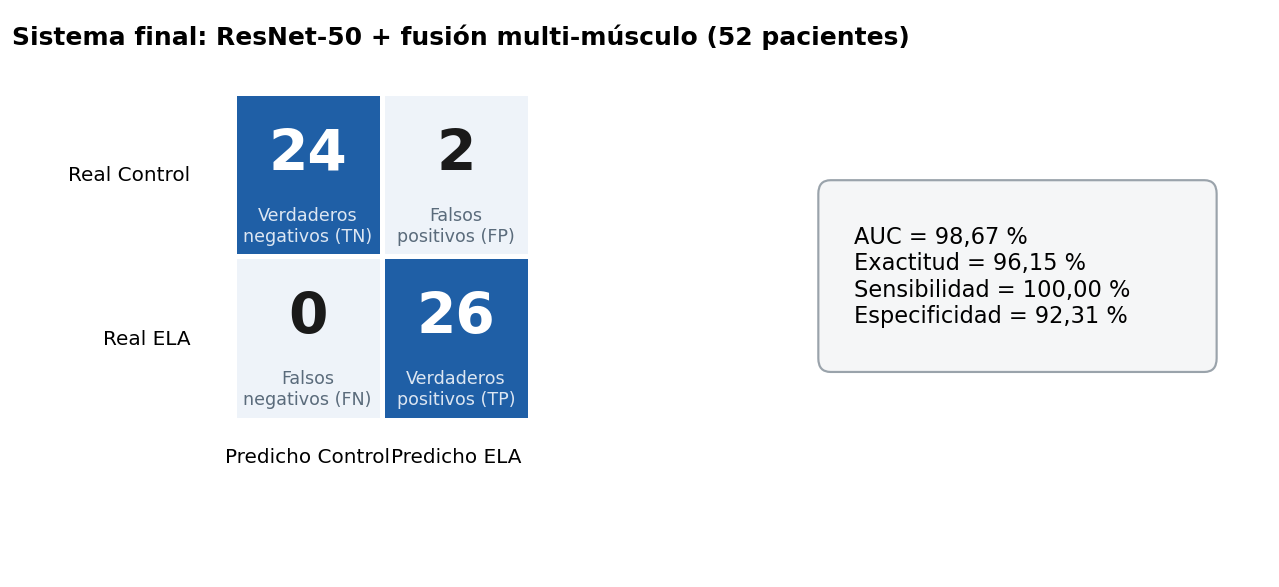
\includegraphics[width=0.7\linewidth]{images/confusion_final.png}
    \caption{Matriz de confusi\'on del sistema final (ResNet-50 con fusi\'on multi-m\'usculo a nivel paciente) sobre los 52 pacientes evaluados \textit{out-of-fold}: 24 verdaderos negativos, 26 verdaderos positivos, ning\'un falso negativo y 2 falsos positivos. Junto a la matriz se resumen las m\'etricas globales (AUC 98{,}67\,\%, exactitud 96{,}15\,\%, sensibilidad 100\,\% y especificidad 92{,}31\,\%).}
    \label{fig:confusion-es}
\end{figure}

\sectionnotoc{Conclusiones}

La aportaci\'on principal del trabajo es la integraci\'on multi-m\'usculo a nivel de paciente, validada con metodolog\'ia estad\'istica rigurosa e interpretada mediante mapas de activaci\'on. El sistema propuesto, reproducible y de c\'odigo abierto, aporta evidencia de que los modelos profundos sobre ecograf\'ia muscular pueden alcanzar un rendimiento cl\'inicamente operativo. Como l\'ineas de trabajo futuro se plantean la validaci\'on externa con cohortes independientes, la calibraci\'on probabil\'istica de las predicciones y la extensi\'on a la monitorizaci\'on longitudinal de la progresi\'on de la enfermedad.

\sectionnotoc{Referencias}

\printbibliography[heading=none]

\end{refsection}

\end{otherlanguage}

\newpage

\resetcounters

%%%%%%%%%%%%%%%%%%%%%%%%%%%%%%%%%%%%%%%%%%%%%%%%%%%%%%%%%%%%%%%%%%%%%%%%%%%%%%%%%%%%%%%%%%%
%% EXECUTIVE SUMMARY IN ENGLISH
%%%%%%%%%%%%%%%%%%%%%%%%%%%%%%%%%%%%%%%%%%%%%%%%%%%%%%%%%%%%%%%%%%%%%%%%%%%%%%%%%%%%%%%%%%%

\begin{otherlanguage}{english}

{\large \MakeUppercase{\projectTitleEnglish}}
\vspace{3mm}

\textbf{Author: \Author}

Director: \Director

\vspace{2mm}
Collaborating entity: Fundaci\'on San Juan de Dios -- ICAI, Universidad Pontificia Comillas

\begin{refsection}[ref_executive_summary.bib]

\section*{Abstract}
Amyotrophic Lateral Sclerosis (ALS) lacks an accessible early diagnostic biomarker. This work develops a deep-learning system that detects ALS from muscle ultrasound, integrating four muscle groups into a patient-level decision. On 52 patients, the system reaches an AUC of 98.67\,\%, a sensitivity of 100\,\% and a specificity of 92.31\,\%, on par with the clinical baseline based on classical textural analysis.

\textbf{Keywords}: Amyotrophic Lateral Sclerosis; muscle ultrasound; deep learning; convolutional neural networks; patient-level fusion; subject-wise cross-validation.

\section*{Executive Summary}

\sectionnotoc{Introduction}

Amyotrophic Lateral Sclerosis (ALS) is a fatal neurodegenerative disease in which early diagnosis remains a clinical challenge: the average delay between the first symptoms and the definitive diagnosis is around twelve months~\cite{hardiman2017als}. Quantitative muscle ultrasonography has been proposed as a non-invasive, low-cost biomarker~\cite{pillen2008muscle}, but its interpretation requires expertise and classical methods, based on hand-crafted textural features, suffer from limited generalisation~\cite{martinezpaya2017quantitative}. This Bachelor's Thesis addresses the automation of muscle texture analysis through deep learning~\cite{litjens2017survey}, integrating the four classically explored muscle groups (biceps, forearm, quadriceps and tibial) into a single diagnostic decision formulated at the patient level.

\sectionnotoc{Objectives}

The main goal is to design and validate an ALS diagnostic support system based on convolutional neural networks applied to muscle ultrasound, operating at the patient level. The specific objectives are: to train and compare five pre-trained architectures; to ensure a methodologically honest validation through subject-wise stratified cross-validation; to quantify uncertainty by means of inferential statistical analysis; to design a multi-muscle fusion strategy at the patient level; to interpret the model's decisions through explainability maps; and to benchmark the overall performance against the clinical baseline.

\sectionnotoc{Description of the Model/System/Tool}

The system starts from five convolutional architectures pre-trained on ImageNet (ResNet-18, ResNet-50, DenseNet-121, EfficientNet-B0 and ConvNeXt-Tiny), fine-tuned via transfer learning on each of the four muscles. Training uses five-fold cross-validation with \texttt{Stratified\allowbreak Group\allowbreak KFold}, which preserves class balance and guarantees that no patient shares images between training and validation. From the out-of-fold predictions, the system aggregates images at the patient-and-muscle level and fuses the four muscles into a single ALS probability. The decision threshold is recalibrated using Youden's J index.

\begin{figure}[H]
    \centering
    \begin{tikzpicture}[
        node distance=4mm and 4mm,
        base/.style={draw, rounded corners=2pt, align=center, font=\footnotesize, inner sep=4pt, minimum height=7mm},
        stage/.style={base, fill=blue!8, minimum width=70mm},
        muscle/.style={base, fill=blue!18, minimum width=15mm},
        cnn/.style={base, fill=orange!18, minimum width=15mm},
        prob/.style={base, fill=white, minimum width=15mm, font=\scriptsize},
        fuse/.style={base, fill=green!18, minimum width=70mm},
        decide/.style={base, fill=green!30, minimum width=70mm, font=\footnotesize\bfseries},
        arr/.style={-{Stealth[length=2mm]}, semithick}
    ]
    \node[stage] (input) {Ultrasound images (.tif) --- 4 muscle groups};
    \node[stage, below=of input] (prep) {Preprocessing: $224\times 224$, ImageNet normalisation};
    \node[stage, below=of prep] (split) {Subject-wise cross-validation (5-fold StratifiedGroupKFold)};

    \node[muscle, below=8mm of split, xshift=-27mm] (m1) {BBr};
    \node[muscle, below=8mm of split, xshift=-9mm]  (m2) {FxM};
    \node[muscle, below=8mm of split, xshift=9mm]   (m3) {Cdr};
    \node[muscle, below=8mm of split, xshift=27mm]  (m4) {TbA};

    \node[cnn, below=of m1] (c1) {ResNet-50};
    \node[cnn, below=of m2] (c2) {ResNet-50};
    \node[cnn, below=of m3] (c3) {ResNet-50};
    \node[cnn, below=of m4] (c4) {ResNet-50};

    \node[prob, below=of c1] (p1) {$P(\text{ALS})$};
    \node[prob, below=of c2] (p2) {$P(\text{ALS})$};
    \node[prob, below=of c3] (p3) {$P(\text{ALS})$};
    \node[prob, below=of c4] (p4) {$P(\text{ALS})$};

    \node[fuse, below=10mm of p2.south, xshift=9mm] (fuse) {Multi-muscle fusion (simple mean) + Youden threshold};
    \node[decide, below=of fuse] (dec) {Patient-level decision: ALS / Control};

    \draw[arr] (input) -- (prep);
    \draw[arr] (prep) -- (split);
    \draw[arr] (split.south) -- (m1.north);
    \draw[arr] (split.south) -- (m2.north);
    \draw[arr] (split.south) -- (m3.north);
    \draw[arr] (split.south) -- (m4.north);
    \draw[arr] (m1) -- (c1); \draw[arr] (m2) -- (c2);
    \draw[arr] (m3) -- (c3); \draw[arr] (m4) -- (c4);
    \draw[arr] (c1) -- (p1); \draw[arr] (c2) -- (p2);
    \draw[arr] (c3) -- (p3); \draw[arr] (c4) -- (p4);
    \draw[arr] (p1.south) -- (fuse.north);
    \draw[arr] (p2.south) -- (fuse.north);
    \draw[arr] (p3.south) -- (fuse.north);
    \draw[arr] (p4.south) -- (fuse.north);
    \draw[arr] (fuse) -- (dec);
    \end{tikzpicture}
    \caption{Overview of the system: from preprocessing of the ultrasound images to the fused patient-level diagnostic decision. BBr = biceps brachii, FxM = forearm flexors, Cdr = quadriceps femoris, TbA = tibialis anterior.}
    \label{fig:pipeline-en}
\end{figure}

\sectionnotoc{Results}

Validation is performed on 52 patients (26 with ALS, 26 controls) using out-of-fold predictions, complemented with 95\,\% confidence intervals obtained by bootstrap. The final system, based on ResNet-50 with simple-mean fusion, reaches an AUC of 98.67\,\% (95\,\%\,CI 95.4--100.0), a sensitivity of 100\,\% and a specificity of 92.31\,\%, with no false negatives and two false positives. The differential contribution of this work is the multi-muscle integration at the patient level, absent in the clinical baseline of Mart\'inez-Pay\'a.

\begin{figure}[H]
    \centering
    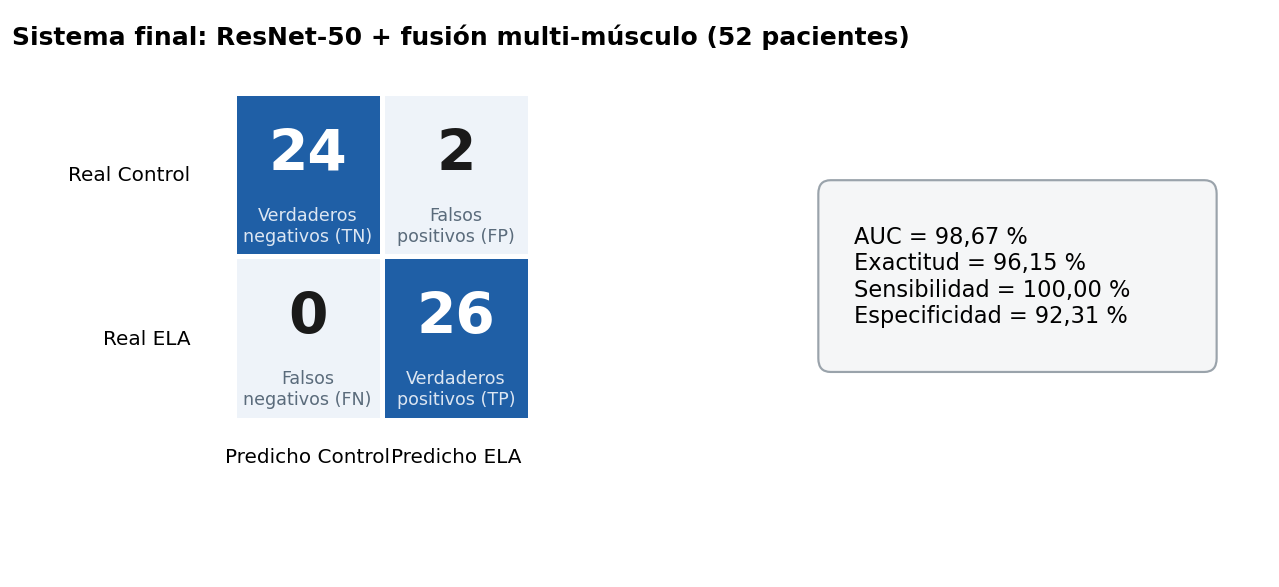
\includegraphics[width=0.7\linewidth]{images/confusion_final.png}
    \caption{Confusion matrix of the final system (ResNet-50 with patient-level multi-muscle fusion) over the 52 patients evaluated out-of-fold: 24 true negatives, 26 true positives, no false negatives and 2 false positives. The global metrics are summarised next to the matrix (AUC 98.67\,\%, accuracy 96.15\,\%, sensitivity 100\,\% and specificity 92.31\,\%).}
    \label{fig:confusion-en}
\end{figure}

\sectionnotoc{Conclusions}

The main contribution of this work is the multi-muscle integration at the patient level, validated with a rigorous statistical methodology and interpreted through activation maps. The proposed system, reproducible and open-source, provides evidence that deep-learning models on muscle ultrasound can reach clinically operational performance. Future work includes external validation on independent cohorts, probabilistic calibration of the predictions and an extension to longitudinal monitoring of disease progression.

\sectionnotoc{References}

\printbibliography[heading=none]

\end{refsection}

\end{otherlanguage}

\newpage

\captionsetup[figure]{list=true}
\captionsetup[table]{list=true}

\tableofcontents
\thispagestyle{fancy}
\newpage
\setcounter{page}{1}
\fancyfoot[C]{
    \begin{center}
        \thepage
    \end{center}
} 
\renewcommand{\footrulewidth}{0.4pt}
\setlength{\footskip}{0.8cm}

\newpage
\selectlanguage{spanish}

\phantomsection
\listoffigures

\newpage

\phantomsection
\listoftables

\newpage

%%%%%%%%%%%%%%%%%%%%%%%%%%%%%%%%%%%%%%%%%%%%%%%%%%%%%%%%
%%%% Introducci\'on %%%%%%%%%%%%%%%%%%%%%%%%%%%%%%%%%%%%%%
%%%%%%%%%%%%%%%%%%%%%%%%%%%%%%%%%%%%%%%%%%%%%%%%%%%%%%%%

\resetcounters


\begin{refsection}[ref_tfg.bib]
\section{Introducci\'on}

La Esclerosis Lateral Amiotr\'ofica (ELA) es una enfermedad neurodegenerativa caracterizada por la degeneraci\'on progresiva de las motoneuronas superior e inferior, que conduce a debilidad muscular, atrofia y, finalmente, fallo respiratorio \cite{brown2017als, hardiman2017als}. Se trata de una patolog\'ia de pron\'ostico fatal, con una supervivencia mediana de entre tres y cinco a\~nos desde la aparici\'on de los primeros s\'intomas. En Europa, su incidencia anual se estima entre 2 y 3 casos por cada 100.000 habitantes \cite{logroscino2010incidence}.

En ausencia de un biomarcador diagn\'ostico espec\'ifico, el diagn\'ostico de la ELA se apoya en los criterios de El Escorial \cite{brooks2000escorial}, que combinan la exploraci\'on cl\'inica con la electromiograf\'ia. Este procedimiento conlleva un retraso medio cercano a los doce meses entre los primeros s\'intomas y el diagn\'ostico definitivo, una ventana temporal cr\'itica en la que la intervenci\'on terap\'eutica podr\'ia tener un mayor impacto. En este contexto, la ecograf\'ia muscular cuantitativa ha emergido como una t\'ecnica de imagen no invasiva, accesible y de bajo coste, capaz de detectar los cambios estructurales que la enfermedad provoca en el tejido muscular \cite{pillen2008muscle, martinezpaya2017quantitative}.

Este Trabajo Fin de Grado propone un sistema basado en aprendizaje profundo que automatiza el an\'alisis de las texturas musculares a partir de im\'agenes ecogr\'aficas, integrando los cuatro grupos musculares cl\'asicamente explorados en una \'unica decisi\'on diagn\'ostica formulada a nivel de paciente.

\subsection{Motivaci\'on}

El an\'alisis de la ecograf\'ia muscular en la ELA se ha abordado tradicionalmente mediante caracter\'isticas texturales calculadas de forma manual --- par\'ametros de la matriz de co-ocurrencia de niveles de gris, ecogenicidad o ecovariaci\'on \cite{martinezpaya2017quantitative, martinezpaya2018monitoring}. Aunque estos m\'etodos han demostrado capacidad discriminativa, presentan dos limitaciones relevantes. En primer lugar, dependen de descriptores dise\~nados a mano que pueden no capturar la totalidad de la informaci\'on presente en la imagen. En segundo lugar, los trabajos previos reportan resultados a nivel de imagen y por m\'usculo de forma aislada, sin proponer una estrategia que integre la exploraci\'on completa del paciente en una \'unica decisi\'on, que es la unidad de inter\'es cl\'inico.

El aprendizaje profundo ha transformado el an\'alisis de imagen m\'edica al permitir que los descriptores se aprendan directamente de los datos \cite{litjens2017survey}. Aplicar este paradigma a la ecograf\'ia muscular en la ELA, y hacerlo de forma metodol\'ogicamente rigurosa y a nivel de paciente, constituye la motivaci\'on central de este trabajo.

\subsection{Objetivos}

El objetivo principal de este Trabajo Fin de Grado es dise\~nar, implementar y validar un sistema de soporte al diagn\'ostico de la ELA, basado en redes neuronales convolucionales aplicadas a la ecograf\'ia muscular, que opere a nivel de paciente. Para alcanzarlo se definen los siguientes objetivos espec\'ificos:

\begin{itemize}
    \item Entrenar y comparar cinco arquitecturas convolucionales pre-entrenadas sobre cada uno de los cuatro m\'usculos analizados.
    \item Garantizar la integridad metodol\'ogica de la validaci\'on mediante validaci\'on cruzada estratificada y agrupada por sujeto, evitando la fuga de informaci\'on entre los conjuntos de entrenamiento y validaci\'on.
    \item Cuantificar la incertidumbre de las m\'etricas obtenidas mediante an\'alisis estad\'istico inferencial: intervalos de confianza, recalibraci\'on de umbral y contrastes de hip\'otesis pareados.
    \item Dise\~nar y validar una estrategia de fusi\'on que integre los cuatro m\'usculos en una \'unica probabilidad de ELA a nivel de paciente.
    \item Generar mapas de explicabilidad que permitan verificar que las decisiones del modelo se sustentan en regiones cl\'inicamente relevantes.
    \item Comparar el rendimiento global del sistema con la l\'inea base cl\'inica vigente.
\end{itemize}

\subsection{Alineaci\'on con los ODS}

Este trabajo se alinea con dos de los \href{https://sdgs.un.org/es/goals}{Objetivos de Desarrollo Sostenible (ODS)} de la Agenda 2030 de Naciones Unidas. El proyecto contribuye principalmente al \textbf{ODS 3 (Salud y Bienestar)}: el sistema desarrollado constituye una herramienta de apoyo diagn\'ostico no invasiva y de bajo coste, en l\'inea con la meta 3.4, orientada a reducir la mortalidad prematura por enfermedades no transmisibles, y con la meta 3.b, de apoyo a la investigaci\'on y el desarrollo de tecnolog\'ias sanitarias. De forma secundaria, el trabajo contribuye al \textbf{ODS 9 (Industria, Innovaci\'on e Infraestructura)}, al materializar la transferencia de t\'ecnicas avanzadas de inteligencia artificial a un dominio cl\'inico tradicionalmente dependiente de la inspecci\'on cualitativa.

\subsection{Estructura del trabajo}

El resto de la memoria se organiza como sigue. El cap\'itulo~\ref{sec:related} revisa el estado del arte, tanto cl\'inico como t\'ecnico, y sit\'ua el trabajo respecto a la literatura previa. El cap\'itulo~\ref{sec:methodology} describe en detalle el sistema desarrollado: el planteamiento del problema, el dise\~no de la soluci\'on y su implementaci\'on. El cap\'itulo~\ref{sec:results} presenta los resultados experimentales y su an\'alisis cr\'itico. Finalmente, el cap\'itulo~\ref{sec:conclusion} recoge las conclusiones del trabajo y las l\'ineas de investigaci\'on futuras.

\newpage

%%%%%%%%%%%%%%%%%%%%%%%%%%%%%%%%%%%%%%%%%%%%%%%%%%%%%%%%
%%%% Trabajos relacionados %%%%%%%%%%%%%%%%%%%%%%%%%%%%%
%%%%%%%%%%%%%%%%%%%%%%%%%%%%%%%%%%%%%%%%%%%%%%%%%%%%%%%%
\section{Estado del arte}\label{sec:related}

Este capítulo revisa el conocimiento previo sobre el que se construye el proyecto. Se parte de los conceptos clínicos de la enfermedad y de la técnica de imagen empleada (secciones~\ref{subsec:ela} y~\ref{subsec:ecografia}), se examina la línea base clínica que ha aplicado análisis cuantitativo de imagen al diagnóstico de la Esclerosis Lateral Amiotrófica (sección~\ref{subsec:linea-base}), se describen las técnicas de aprendizaje profundo relevantes para el problema (sección~\ref{subsec:dl}) y se discuten los retos metodológicos asociados a la validación con conjuntos de datos clínicos reducidos (sección~\ref{subsec:validacion}). El capítulo concluye identificando el vacío en la literatura que justifica el presente trabajo (sección~\ref{subsec:gap}).

\subsection{La Esclerosis Lateral Amiotrófica}\label{subsec:ela}

La Esclerosis Lateral Amiotrófica (ELA) es una enfermedad neurodegenerativa caracterizada por la pérdida progresiva de las motoneuronas superiores e inferiores, lo que provoca debilidad muscular, atrofia y, en última instancia, parálisis y fallo respiratorio \cite{brown2017als,hardiman2017als}. Su incidencia anual en las poblaciones europeas se estima entre 2 y 3 casos por cada 100.000 habitantes, y la supervivencia mediana desde el inicio de los síntomas es de tres a cinco años \cite{logroscino2010incidence,hardiman2017als}.

El diagnóstico de la ELA es eminentemente clínico y se apoya en los criterios de El Escorial y sus revisiones posteriores, que combinan la exploración neurológica con estudios electrofisiológicos para confirmar la afectación de la motoneurona en distintas regiones corporales \cite{brooks2000escorial}. Estos criterios fueron concebidos con fines de investigación y exigen una afectación ya extendida, por lo que su sensibilidad en las fases iniciales es limitada. En la práctica clínica esto se traduce en un retraso diagnóstico medio de entre diez y dieciséis meses desde la aparición de los primeros síntomas \cite{hardiman2017als}. Dado que el deterioro neuronal es irreversible y que las terapias disponibles son más eficaces cuanto antes se instauran, reducir ese retraso constituye una necesidad clínica de primer orden y motiva la búsqueda de marcadores objetivos, accesibles y no invasivos que apoyen la sospecha diagnóstica.

\subsection{Ecografía muscular cuantitativa}\label{subsec:ecografia}

La ecografía muscular ha emergido como una herramienta complementaria en la evaluación de las enfermedades neuromusculares. Frente a la electromiografía, que es dolorosa e invasiva, y frente a la resonancia magnética, costosa y de disponibilidad limitada, la ecografía es indolora, de bajo coste, portátil y permite explorar varios músculos en una misma sesión \cite{pillen2008muscle}. Cuando una enfermedad neuromuscular sustituye tejido muscular sano por tejido fibroso y graso, la cantidad de ultrasonidos reflejados aumenta y el músculo aparece más brillante en la imagen. Esta propiedad se cuantifica mediante la \textit{ecointensidad}, definida como el nivel medio de gris del músculo en una región de interés \cite{pillen2008muscle,arts2010normal}.

El uso clínico de la ecointensidad presenta, sin embargo, limitaciones conocidas. Su valor depende del equipo, de los ajustes del ecógrafo y del operador, lo que obliga a disponer de valores de referencia normalizados por edad y por músculo \cite{arts2010normal}. Además, la ecointensidad media resume en un único número toda la información de la imagen y descarta la organización espacial de los píxeles, es decir, la \textit{textura} del músculo. Esta observación ha impulsado el desarrollo de métodos de análisis textural cuantitativo, que extraen descriptores estadísticos de los patrones de gris de la imagen con el objetivo de capturar alteraciones que la ecointensidad media no refleja.

\subsection{Línea base clínica: análisis textural en la ELA}\label{subsec:linea-base}

El grupo de Martínez-Payá y colaboradores constituye la referencia más directa para este trabajo. En un primer estudio, los autores demostraron que descriptores de textura extraídos de ecografías de músculos de pacientes con ELA permitían diferenciarlos de sujetos sanos, estableciendo que la imagen muscular contiene información discriminante más allá de la ecointensidad media \cite{martinezpaya2017quantitative}. Trabajos posteriores del mismo grupo confirmaron que estos descriptores también reflejan la progresión de la enfermedad a lo largo del tiempo \cite{martinezpaya2018monitoring}. Más recientemente, esta línea de investigación se ha extendido a nuevas cohortes y conjuntos musculares \cite{aljaro2026quantitative}.

Estos trabajos comparten un mismo esquema metodológico: las características de textura se calculan mediante fórmulas estadísticas predefinidas (matrices de coocurrencia, dimensión fractal, descriptores de la transformada wavelet, entre otros) y se seleccionan e introducen después en clasificadores estadísticos clásicos. Este enfoque, que puede denominarse de \textit{ingeniería manual de características}, tiene la ventaja de la interpretabilidad, pero presenta una limitación de fondo: el conjunto de descriptores se fija de antemano y, por tanto, el sistema sólo puede detectar aquellos patrones que el experto ha decidido cuantificar. Cualquier patrón discriminante no contemplado en la batería de fórmulas queda fuera del alcance del modelo. Esta limitación es precisamente la que motiva explorar técnicas capaces de aprender las características relevantes directamente de los datos.

\subsection{Aprendizaje profundo en imagen médica}\label{subsec:dl}

Las redes neuronales convolucionales (CNN) invierten el paradigma del análisis textural manual: en lugar de calcular descriptores fijados de antemano, aprenden de los propios datos qué patrones de la imagen son relevantes para la tarea \cite{krizhevsky2012imagenet}. Desde su irrupción, las CNN se han convertido en el estándar para tareas de clasificación de imagen y han sido adoptadas de forma generalizada en el análisis de imagen médica \cite{litjens2017survey,shen2017deep}.

El principal obstáculo para aplicar aprendizaje profundo en el ámbito clínico es la escasez de datos: entrenar una CNN desde cero requiere decenas de miles de imágenes etiquetadas, una cifra inalcanzable en la mayoría de los estudios médicos. La solución habitual es el \textit{aprendizaje por transferencia} (\textit{transfer learning}), que consiste en partir de una red preentrenada sobre un gran corpus de imágenes naturales —típicamente ImageNet \cite{deng2009imagenet}— y reajustarla sobre el conjunto de datos específico. Las primeras capas de una CNN aprenden detectores de bordes, texturas y formas que son en buena medida genéricos y reutilizables entre dominios \cite{yosinski2014transferable}, lo que hace de esta estrategia la opción de referencia cuando el conjunto de datos es pequeño, como han confirmado numerosos estudios en imagen médica \cite{tajbakhsh2016convolutional,litjens2017survey}.

A lo largo de la última década se han propuesto sucesivas arquitecturas de CNN que han mejorado progresivamente el rendimiento y la eficiencia. ResNet introdujo las conexiones residuales, que permiten entrenar redes muy profundas evitando la degradación del gradiente \cite{he2016deep}. DenseNet llevó esta idea más lejos conectando cada capa con todas las posteriores, lo que favorece la reutilización de características \cite{huang2017densely}. EfficientNet propuso un escalado equilibrado de la profundidad, la anchura y la resolución de la red para maximizar la precisión por parámetro \cite{tan2019efficientnet}. Por último, ConvNeXt reexaminó el diseño convolucional incorporando elementos de los \textit{transformers} de visión, alcanzando un rendimiento competitivo con un esquema puramente convolucional \cite{liu2022convnet}. La existencia de familias de arquitecturas con compromisos distintos entre capacidad, eficiencia y riesgo de sobreajuste justifica que un estudio sobre un dominio nuevo compare varias de ellas en lugar de comprometerse con una sola a priori. La tabla~\ref{tab:arquitecturas} resume las características principales de las cinco arquitecturas comparadas en este trabajo, y los párrafos siguientes desarrollan brevemente las ideas centrales de cada familia.

\begin{table}[H]
\centering
\caption{Resumen comparativo de las cinco arquitecturas convolucionales empleadas en este trabajo. Los parámetros se reportan en millones para la variante específica utilizada.}
\label{tab:arquitecturas}
\small
\begin{tabular}{lcll}
\toprule
\textbf{Arquitectura} & \textbf{Año} & \textbf{Parámetros} & \textbf{Idea principal} \\
\midrule
ResNet-18       & 2016 & $\sim$11~M & Conexiones residuales (\textit{skip connections}) \\
ResNet-50       & 2016 & $\sim$26~M & ResNet con bloques \textit{bottleneck} más profundos \\
DenseNet-121    & 2017 & $\sim$7~M  & Concatenación densa entre capas \\
EfficientNet-B0 & 2019 & $\sim$5~M  & Escalado balanceado profundidad/anchura/resolución \\
ConvNeXt-Tiny   & 2022 & $\sim$28~M & CNN moderna inspirada en \textit{vision transformers} \\
\bottomrule
\end{tabular}
\end{table}

\textbf{ResNet} \cite{he2016deep} (\textit{residual networks}) resolvió uno de los problemas centrales del entrenamiento de redes profundas: a partir de cierta profundidad, añadir capas dejaba de mejorar el rendimiento y, paradójicamente, lo empeoraba. La causa no era el sobreajuste, sino una dificultad de optimización: los gradientes se atenuaban antes de llegar a las capas iniciales. La solución propuesta consiste en añadir conexiones de salto (\textit{skip connections}) que cortocircuitan dos o tres capas, de modo que cada bloque aprende un residuo $\Delta x = F(x)$ en lugar de la representación completa $H(x) = x + F(x)$. Esta reformulación facilita el aprendizaje de la identidad como punto de partida y permite entrenar redes de cientos de capas. Las variantes ResNet-18 y ResNet-50 se diferencian en el número de bloques y, sobre todo, en su tipo: la primera utiliza bloques sencillos con dos convoluciones $3\times 3$, mientras que la segunda usa bloques \textit{bottleneck} con tres convoluciones ($1\times 1$, $3\times 3$, $1\times 1$) que reducen y restauran la dimensionalidad de los canales, ahorrando cómputo. ResNet-50 es históricamente la línea base de referencia para experimentos de \textit{transfer learning} sobre ImageNet, y por eso se ha incluido en este trabajo.

\textbf{DenseNet} \cite{huang2017densely} llevó la idea de las conexiones de salto a un extremo: en lugar de saltar dos o tres capas, cada capa recibe como entrada la concatenación de las salidas de \textit{todas} las capas anteriores dentro del mismo \textit{dense block}. Esta conectividad densa cumple tres funciones simultáneas: refuerza la propagación de las características, mitiga el problema de los gradientes y reduce drásticamente el número de parámetros necesarios, porque las capas profundas no necesitan re-aprender las características ya extraídas por capas previas. DenseNet-121 logra rendimientos comparables a ResNet-50 con apenas siete millones de parámetros, una característica deseable en escenarios de pocos datos donde el riesgo de sobreajuste es elevado.

\textbf{EfficientNet} \cite{tan2019efficientnet} introduce una idea distinta: en lugar de proponer una arquitectura concreta, los autores formulan un \textit{compound scaling} que escala simultáneamente la profundidad, la anchura y la resolución de entrada de la red con un único coeficiente. La intuición es que escalar una sola de las tres dimensiones, como había sido habitual, no aprovecha de forma óptima el presupuesto computacional. EfficientNet-B0 es la red base del escalado, optimizada mediante \textit{neural architecture search}. Con cinco millones de parámetros, ofrece una eficiencia notable: alcanza precisiones equivalentes a redes mucho más grandes con una fracción del cómputo, lo que la convierte en una alternativa interesante cuando el conjunto de datos es modesto.

\textbf{ConvNeXt} \cite{liu2022convnet} responde a una pregunta especialmente relevante tras la irrupción de los \textit{vision transformers} (ViT): ¿es la naturaleza convolucional la que limita el rendimiento, o lo son únicamente sus elecciones de diseño históricas? Los autores construyen progresivamente una CNN moderna incorporando, una a una, las decisiones de diseño que distinguen a los ViT: \textit{patchify} en lugar de convolución agresiva inicial, normalización por capa (LayerNorm) en lugar de \textit{batch normalization}, activación GELU en lugar de ReLU, mayor proporción entre la dimensión interna y la externa del bloque, etc. ConvNeXt-Tiny es el resultado de esa modernización a escala pequeña; con 28 millones de parámetros, iguala o supera a ViT-Base manteniendo el sesgo inductivo convolucional, especialmente útil cuando el conjunto de datos es limitado y no permite que un \textit{transformer} aprenda desde cero las invarianzas espaciales que una CNN incorpora por construcción.

\textbf{Selección de las arquitecturas para este trabajo.} La elección de las cinco arquitecturas anteriores busca cubrir el espacio de soluciones modernas con compromisos distintos. ResNet-18 y ResNet-50 representan la referencia residual a dos escalas. DenseNet-121 aporta una opción densa de pocos parámetros. EfficientNet-B0 explora la eficiencia escalada. ConvNeXt-Tiny incorpora las lecciones del paradigma \textit{transformer} dentro de un marco convolucional. Se descartaron explícitamente dos candidatas habituales en comparativas anteriores: VGG-16, por su excesivo número de parámetros ($\sim$138 millones) que la hace particularmente propensa al sobreajuste sobre 104 imágenes por músculo; y MobileNet-V3 Small, por solapar funcionalmente con EfficientNet-B0 en el rol de arquitectura moderna y compacta sin aportar una perspectiva diferenciada para los objetivos del trabajo.

Una objeción recurrente al uso de aprendizaje profundo en medicina es su naturaleza de «caja negra». Para mitigarla se han desarrollado técnicas de explicabilidad que permiten visualizar qué regiones de la imagen sustentan la predicción del modelo, como la retropropagación guiada \cite{springenberg2015striving}, los mapas de saliencia \cite{simonyan2014deep}, la visualización de activaciones \cite{zeiler2014visualizing} y, en particular, Grad-CAM \cite{selvaraju2017gradcam}, que genera mapas de calor superpuestos a la imagen original. Estas herramientas resultan imprescindibles para que un modelo sea verificable y aceptable en un contexto clínico.

\subsection{Retos de validación en conjuntos de datos clínicos reducidos}\label{subsec:validacion}

Aplicar aprendizaje profundo a un conjunto de datos clínico pequeño no sólo plantea un reto de entrenamiento, sino sobre todo un reto de validación. Con pocas muestras, una única partición en entrenamiento y test produce estimaciones de rendimiento muy inestables, por lo que se recurre a la validación cruzada, que promedia el rendimiento sobre varias particiones y aprovecha todos los datos disponibles \cite{kohavi1995study}.

El riesgo más grave y a la vez más sutil en estos escenarios es la \textit{fuga de información} (\textit{data leakage}). En estudios de imagen médica es habitual disponer de varias imágenes por paciente; si imágenes de un mismo paciente quedan repartidas entre los conjuntos de entrenamiento y de evaluación, el modelo puede aprender a reconocer al individuo en lugar de la enfermedad, y el rendimiento medido resulta optimista y no generalizable \cite{saeb2017need}. La literatura ha documentado de forma reiterada este y otros errores metodológicos —ausencia de agrupación por paciente, selección de características antes de particionar, recalibración de umbrales sobre el conjunto de test— como causas frecuentes de resultados irreproducibles en aprendizaje automático aplicado a la medicina \cite{roberts2021common}. La prevención de la fuga exige que la partición se realice a nivel de paciente, garantizando que todas las imágenes de un individuo permanezcan en el mismo subconjunto.

La comparación rigurosa de modelos sobre conjuntos pequeños requiere asimismo un instrumental estadístico adecuado. El área bajo la curva ROC (AUC) es la métrica de referencia para cuantificar la capacidad discriminante de un clasificador \cite{hanley1982meaning}; la prueba de DeLong permite comparar dos AUC calculadas sobre la misma muestra teniendo en cuenta su correlación \cite{delong1988comparing}; la prueba de los rangos con signo de Wilcoxon ofrece una alternativa no paramétrica para comparar rendimientos emparejados \cite{wilcoxon1945individual}; el índice J de Youden proporciona un criterio objetivo para fijar el umbral de decisión \cite{youden1950index}; y los métodos de remuestreo \textit{bootstrap} permiten estimar intervalos de confianza sin asumir una distribución concreta \cite{efron1979bootstrap,efron1993introduction}. El empleo conjunto de estas herramientas es lo que distingue una comparación de modelos metodológicamente sólida de una mera ordenación por rendimiento.

\subsection{Limitaciones del estado del arte y justificación del proyecto}\label{subsec:gap}

De la revisión anterior se desprenden dos observaciones que, en conjunto, definen el vacío que aborda este trabajo. Por un lado, el análisis cuantitativo de la ecografía muscular en la ELA se ha apoyado hasta la fecha en descriptores de textura diseñados manualmente \cite{martinezpaya2017quantitative,martinezpaya2018monitoring}, un enfoque limitado por definición a los patrones que el experto decide cuantificar. Por otro lado, el aprendizaje profundo —capaz de aprender esas características directamente de los datos y consolidado ya en numerosas modalidades de imagen médica \cite{litjens2017survey,shen2017deep}— no se ha aplicado, hasta donde alcanza esta revisión, a la detección de la ELA a partir de ecografía muscular.

Este trabajo se sitúa precisamente en esa intersección. Su aportación es doble. En primer lugar, aplica y compara de forma sistemática varias arquitecturas modernas de CNN sobre ecografías musculares de pacientes con ELA, sustituyendo la ingeniería manual de características por características aprendidas. En segundo lugar, lo hace bajo un protocolo de validación diseñado expresamente para el escenario de datos clínicos reducidos: partición agrupada por paciente para evitar la fuga de información, validación cruzada estratificada y comparación estadística rigurosa frente a la línea base clínica de Martínez-Payá. El capítulo siguiente describe en detalle la metodología con la que se materializa esta propuesta.

\newpage


%%%%%%%%%%%%%%%%%%%%%%%%%%%%%%%%%%%%%%%%%%%%%%%%%%%%%%%%
%%%% Metodolog\'ia %%%%%%%%%%%%%%%%%%%%%%%%%%%%%%%%%%%%%%%
%%%%%%%%%%%%%%%%%%%%%%%%%%%%%%%%%%%%%%%%%%%%%%%%%%%%%%%%
\section{Metodolog\'ia}\label{sec:methodology}

Este capítulo describe en detalle el sistema desarrollado. La sección~\ref{subsec:planteamiento} formaliza el problema de clasificación, fija los requisitos y define las métricas de evaluación. La sección~\ref{subsec:diseno} presenta el diseño de la solución: el enfoque metodológico, el conjunto de datos, las arquitecturas comparadas, el protocolo de validación cruzada, el esquema de fusión a nivel de paciente y el análisis estadístico. La sección~\ref{subsec:implementacion} detalla la implementación: las tecnologías empleadas, la estructura del código, el flujo de procesamiento y las medidas adoptadas para garantizar la reproducibilidad.

\subsection{Planteamiento del problema}\label{subsec:planteamiento}

\subsubsection{Definición formal}

El problema se aborda en dos niveles encadenados. En el \textbf{nivel de imagen}, se trata de una tarea de clasificación binaria supervisada: dada una imagen de ecografía muscular $x$, el sistema debe estimar la probabilidad $P(\text{ELA}\mid x)$ de que el músculo represente a un paciente con Esclerosis Lateral Amiotrófica, y asignar una etiqueta $y \in \{\text{Control}, \text{ELA}\}$. Formalmente, se busca una función $f_\theta: \mathcal{X} \rightarrow [0,1]$, parametrizada por los pesos $\theta$ de una red neuronal convolucional, que aproxime la probabilidad a posteriori de la clase ELA.

En el \textbf{nivel de paciente}, que es el objetivo clínico último, el sistema dispone de varias imágenes del mismo individuo correspondientes a distintos músculos y debe emitir un único veredicto. Si $\mathcal{I}_p$ denota el conjunto de imágenes del paciente $p$, se busca una función de agregación $g$ tal que $\hat{y}_p = g\bigl(\{f_\theta(x) : x \in \mathcal{I}_p\}\bigr)$ produzca una decisión robusta a partir de la evidencia parcial de cada músculo. La distinción entre ambos niveles es esencial: el modelo se entrena y se valida sobre imágenes, pero la utilidad clínica se mide sobre pacientes.

\subsubsection{Requisitos}

El sistema debe satisfacer un conjunto de requisitos que condicionan todas las decisiones de diseño posteriores. Como \textit{requisitos funcionales}, el sistema debe aceptar como entrada imágenes de ecografía muscular en escala de gris, producir una estimación de probabilidad de ELA tanto por imagen como por paciente, y ofrecer un mecanismo de interpretación visual que permita verificar en qué regiones de la imagen se apoya la predicción. Como \textit{requisitos no funcionales}, la evaluación debe estar libre de fuga de información a nivel de paciente; el protocolo experimental debe ser íntegramente reproducible; los resultados deben ser comparables con la línea base clínica de Martínez-Payá \cite{martinezpaya2017quantitative}; y el sistema debe operar con un conjunto de datos reducido, lo que descarta el entrenamiento de redes desde cero y obliga a recurrir al aprendizaje por transferencia.

\subsubsection{Métricas de evaluación}

Dado que el conjunto de datos está balanceado entre clases, la métrica principal es el \textbf{área bajo la curva ROC} (AUC), que cuantifica la capacidad discriminante del modelo con independencia del umbral de decisión \cite{hanley1982meaning}. El AUC admite una interpretación probabilística directa: es la probabilidad de que, ante un paciente con ELA y un control elegidos al azar, el modelo asigne mayor puntuación al primero. Como métricas complementarias, orientadas a la interpretación clínica, se reportan la \textbf{sensibilidad} (proporción de pacientes con ELA correctamente identificados), la \textbf{especificidad} (proporción de controles correctamente identificados) y la \textbf{exactitud} (\textit{accuracy}). A partir de la matriz de confusión, con verdaderos positivos $TP$, verdaderos negativos $TN$, falsos positivos $FP$ y falsos negativos $FN$, estas métricas se definen como

\begin{equation}
\text{Sens} = \frac{TP}{TP + FN}, \qquad
\text{Spec} = \frac{TN}{TN + FP}, \qquad
\text{Acc} = \frac{TP + TN}{TP + TN + FP + FN}.
\end{equation}

La sensibilidad y la especificidad dependen del umbral que convierte la probabilidad continua en una decisión binaria. Como ese umbral no tiene por qué ser $0{,}5$, se recalibra mediante el \textbf{índice J de Youden} \cite{youden1950index}, definido como $J = \text{Sens} + \text{Spec} - 1$, eligiendo el umbral que maximiza $J$. El AUC, en cambio, es independiente del umbral, lo que lo hace idóneo como criterio principal para comparar arquitecturas.

\subsection{Diseño de la solución}\label{subsec:diseno}

\subsubsection{Enfoque propuesto}

El enfoque propuesto sustituye la ingeniería manual de características de la línea base clínica por características aprendidas directamente de los datos mediante redes neuronales convolucionales. Dado el tamaño reducido del conjunto de datos, no se entrena ninguna red desde cero: todas las arquitecturas parten de pesos preentrenados sobre ImageNet \cite{deng2009imagenet} y se reajustan al problema concreto (aprendizaje por transferencia). Como en este dominio no existe una arquitectura de referencia, no se compromete el trabajo con una sola red, sino que se comparan cinco arquitecturas representativas bajo idéntico protocolo. La evaluación se realiza mediante validación cruzada agrupada por paciente, lo que evita la fuga de información, y los modelos por músculo se combinan después en un único veredicto por paciente mediante reglas de fusión. Finalmente, todas las comparaciones —entre arquitecturas y frente a la línea base— se someten a contraste estadístico, y las predicciones se acompañan de mapas de interpretación visual.

El sistema se organiza en cinco etapas encadenadas: (1) preparación y preprocesado de los datos, (2) entrenamiento de cada arquitectura sobre cada músculo con validación cruzada, (3) análisis estadístico de los resultados por músculo, (4) fusión de los cuatro músculos en una decisión a nivel de paciente y (5) generación de explicaciones visuales sobre el modelo final.

\subsubsection{Conjunto de datos}

El conjunto de datos procede de un estudio de ecografía musculoesquelética y está formado por imágenes de cuatro músculos: el bíceps braquial (\textit{BBr}), los flexores del antebrazo (\textit{FxM}), el cuádriceps femoral (\textit{Cdr}) y el tibial anterior (\textit{TbA}). Para cada músculo se dispone de regiones de interés (ROI) ya segmentadas, exportadas en formato TIFF, correspondientes a $52$ imágenes de sujetos control y $52$ de pacientes con ELA, lo que suma $104$ imágenes por músculo y $416$ imágenes en total. El conjunto está, por tanto, perfectamente balanceado entre clases. A nivel de paciente, el estudio agrupa $52$ individuos ($26$ con ELA y $26$ controles), cada uno con imágenes de los cuatro músculos y de ambos lados del cuerpo (dos imágenes por músculo, lado derecho e izquierdo).

Un aspecto crítico del conjunto de datos es la identificación del paciente. Los nombres de fichero codifican el identificador del sujeto, que se extrae mediante una expresión regular para poder agrupar todas las imágenes de un mismo individuo. Esta identificación es la que permite realizar particiones a nivel de paciente y, con ello, prevenir la fuga de información descrita en el capítulo anterior.

\subsubsection{Arquitecturas comparadas}

Se comparan cinco arquitecturas de red neuronal convolucional, todas ellas preentrenadas sobre ImageNet y adaptadas al problema sustituyendo su capa de clasificación final por una capa lineal de dos salidas. La selección busca cubrir distintos compromisos entre capacidad, eficiencia y riesgo de sobreajuste. \textbf{ResNet-18} y \textbf{ResNet-50} \cite{he2016deep} representan, respectivamente, una variante ligera y una de capacidad media de la familia residual. \textbf{DenseNet-121} \cite{huang2017densely} maximiza la reutilización de características mediante conexiones densas entre capas. \textbf{EfficientNet-B0} \cite{tan2019efficientnet} aporta un diseño optimizado para obtener la máxima precisión por parámetro. \textbf{ConvNeXt-Tiny} \cite{liu2022convnet} incorpora elementos de diseño de los \textit{transformers} de visión manteniendo la naturaleza convolucional. Se descartaron deliberadamente VGG-16, por su elevado número de parámetros ($\sim$138 millones) y el consiguiente riesgo de sobreajuste sobre un conjunto pequeño, y MobileNet-V3, por resultar redundante con EfficientNet-B0 en el papel de arquitectura moderna y eficiente.

\subsubsection{Protocolo de validación cruzada}

Con un conjunto de datos tan reducido, una única partición entrenamiento/test produce estimaciones de rendimiento muy inestables. Por ello se emplea \textbf{validación cruzada de 5 particiones} (\textit{5-fold cross-validation}) \cite{kohavi1995study}, que promedia el rendimiento sobre cinco repeticiones y aprovecha todos los datos disponibles. La partición concreta utilizada es \texttt{Stratified\allowbreak Group\allowbreak KFold}, que combina dos restricciones simultáneas: la \textit{estratificación}, que conserva la proporción de clases Control/ELA en cada partición, y la \textit{agrupación por paciente}, que garantiza que todas las imágenes de un mismo individuo permanezcan en la misma partición. Esta segunda restricción es la salvaguarda frente a la fuga de información: impide que el modelo vea en entrenamiento una imagen de un paciente y sea evaluado después sobre otra imagen del mismo paciente. El proceso se repite de forma independiente para cada una de las veinte combinaciones de arquitectura y músculo, y para cada combinación se obtienen cinco valores de AUC —uno por partición— sobre los que se construyen los intervalos de confianza y los contrastes estadísticos.

La figura~\ref{fig:kfold-schema} ilustra esquemáticamente cómo se distribuyen los 52 pacientes en los cinco \textit{folds}. La estratificación reparte las clases (Control y ELA) en proporciones cercanas a la global ($50$\,\% control y $50$\,\% ELA) dentro de cada partición; la agrupación por paciente impide que sus dos lateralidades (\textit{d} e \textit{i}) o sus posibles tomas repetidas queden en lados opuestos del corte. En cada uno de los cinco entrenamientos, cuatro \textit{folds} se dedican al entrenamiento y el restante a la validación; tras la rotación completa, todos los pacientes han actuado exactamente una vez como conjunto de validación. Esta propiedad es la que habilita la inferencia \textit{out-of-fold} utilizada después en la fusión a nivel paciente.

\begin{figure}[H]
\centering
\begin{tikzpicture}[
    box/.style={draw, minimum height=8mm, font=\scriptsize, align=center, inner sep=2pt},
    val/.style={box, fill=orange!30, minimum width=22mm},
    trn/.style={box, fill=blue!10, minimum width=22mm},
    label/.style={font=\footnotesize, anchor=east},
    title/.style={font=\footnotesize\bfseries, anchor=south}
]
\node[title] at (0, 0.6) {Iteración / \textit{fold}};
\foreach \i/\valpos in {1/0,2/1,3/2,4/3,5/4}{
    \node[label] at (-0.2, -\i*0.7) {Fold \i};
    \foreach \k in {0,1,2,3,4}{
        \pgfmathparse{\k == \valpos ? "val" : "trn"}
        \edef\style{\pgfmathresult}
        \node[\style] at (0.6 + \k*2.4, -\i*0.7) {%
            \ifnum\k=\valpos%
                Validación%
            \else%
                Entrenamiento%
            \fi};
    }
}
% leyenda
\node[val, minimum width=18mm] at (1.7, -5.0) {Validación};
\node[trn, minimum width=18mm] at (5.0, -5.0) {Entrenamiento};
\node[font=\scriptsize, anchor=west] at (-0.5, -5.6) {Cada bloque agrupa $\sim$10-11 pacientes ($\sim$22 imágenes) con balance Control/ELA preservado por estratificación.};
\end{tikzpicture}
\caption{Distribución de los 52 pacientes en los cinco \textit{folds} de la validación cruzada \texttt{Stratified\allowbreak Group\allowbreak KFold}. En cada iteración, cuatro \textit{folds} (azul) se usan para entrenamiento y el restante (naranja) para validación. Tras las cinco iteraciones, cada paciente ha pasado exactamente una vez por validación, lo que permite construir las predicciones \textit{out-of-fold} a nivel paciente.}
\label{fig:kfold-schema}
\end{figure}

\paragraph{Justificación de los hiperparámetros.} Los hiperparámetros del entrenamiento se eligen siguiendo criterios estandarizados para \textit{transfer learning} sobre conjuntos clínicos pequeños. La \textbf{tasa de aprendizaje inicial} $10^{-4}$ es el valor habitualmente recomendado para Adam cuando se parte de pesos preentrenados; valores más altos (típicos en entrenamientos desde cero) tienden a destruir las características aprendidas en ImageNet, mientras que valores significativamente más bajos prolongan el entrenamiento sin ganancia en rendimiento. El \textbf{tamaño de lote 16} es un compromiso entre estabilidad del gradiente y la memoria limitada disponible para entrenamientos en MPS. El \textbf{tope de 50 épocas} actúa como cota superior conservadora: en los 100 entrenamientos realizados, la mejor AUC en validación se alcanza con mediana en la época 8 y un 83\,\% de los \textit{checkpoint} óptimos por debajo de la época 20, lo que confirma que el tope no constituye un cuello de botella sino un margen amplio para la activación del planificador. La \textbf{paciencia de 5 épocas} del \texttt{Reduce\allowbreak LROn\allowbreak Plateau} permite que el planificador reaccione a estancamientos cortos sin sobrerreaccionar a oscilaciones puntuales del AUC en validación, y el \textbf{factor 0,5} para la reducción de la tasa es el estándar de \texttt{scikit-learn} y \texttt{PyTorch} para este tipo de planificador. La \textbf{selección del \textit{checkpoint} por mayor AUC en validación}, en lugar de por exactitud o por la última época, es preferible en conjuntos pequeños y balanceados porque el AUC se sustenta sobre las 22 predicciones probabilísticas completas y es menos sensible a la decisión binaria que puede oscilar por una sola imagen mal clasificada. Finalmente, el \textbf{aumento de datos} —con sus rangos concretos de rotación ($\pm 10^{\circ}$), brillo/contraste ($\pm 0{,}2$) y traslación afín ($\pm 5$\,\%)— se ha calibrado para reflejar la variabilidad operativa típica de la sonda y del protocolo de adquisición sin alterar el contenido textural relevante para el diagnóstico.

\subsubsection{Fusión a nivel de paciente}

Los modelos por músculo producen predicciones a nivel de imagen, pero la decisión clínica se toma sobre el paciente. La fusión combina la evidencia de los cuatro músculos en dos pasos. En el primero, para cada paciente y cada músculo se promedian las probabilidades $P(\text{ELA})$ de todas sus imágenes en ese músculo. Es esencial que estas probabilidades sean \textit{out-of-fold}: se obtienen siempre del modelo de la partición en la que el paciente quedó en validación, de modo que ninguna predicción procede de un modelo que haya visto a ese paciente durante el entrenamiento. En el segundo paso se fusionan las hasta cuatro probabilidades musculares de cada paciente mediante tres reglas. La \textbf{media simple} promedia las cuatro probabilidades con igual peso. La \textbf{media ponderada} las promedia ponderando cada músculo por el AUC alcanzado por su modelo, de manera que los músculos más discriminantes pesan más:

\begin{equation}
P_{\text{fus}} = \frac{\sum_{m} w_m \, P_m}{\sum_{m} w_m}, \qquad w_m = \text{AUC}_m .
\end{equation}

La tercera regla, el \textbf{voto mayoritario}, binariza primero la probabilidad de cada músculo con umbral $0{,}5$ y declara ELA si al menos tres de los cuatro músculos votan ELA. Sobre la probabilidad fusionada de las dos primeras reglas se aplica el umbral de Youden para obtener la decisión final, y la incertidumbre se cuantifica mediante un intervalo de confianza al 95\,\% obtenido por \textit{bootstrap} a nivel de paciente. Es importante destacar que la fusión no entrena ningún modelo nuevo: se limita a agregar predicciones ya existentes, por lo que no introduce sobreajuste adicional. La figura~\ref{fig:fusion-schema} resume el flujo completo de agregación.

\begin{figure}[H]
    \centering
    \begin{tikzpicture}[
        node distance=4mm and 3mm,
        base/.style={draw, rounded corners=2pt, align=center, font=\footnotesize, inner sep=4pt, minimum height=7mm},
        img/.style={base, fill=blue!8, minimum width=22mm, font=\scriptsize},
        agg/.style={base, fill=orange!18, minimum width=22mm, font=\scriptsize},
        fuse/.style={base, fill=green!18, minimum width=58mm},
        decide/.style={base, fill=green!30, minimum width=58mm, font=\footnotesize\bfseries},
        arr/.style={-{Stealth[length=2mm]}, semithick}
    ]
    % Fila 1: Imágenes por músculo (varias por músculo)
    \node[img] (i1) {Imágenes BBr\\(varias)};
    \node[img, right=of i1] (i2) {Imágenes FxM\\(varias)};
    \node[img, right=of i2] (i3) {Imágenes Cdr\\(varias)};
    \node[img, right=of i3] (i4) {Imágenes TbA\\(varias)};
    % Fila 2: Probabilidad por (paciente, músculo) = media de imágenes
    \node[agg, below=8mm of i1] (a1) {$P_{\text{BBr}}$ paciente\\media OOF};
    \node[agg, below=8mm of i2] (a2) {$P_{\text{FxM}}$ paciente\\media OOF};
    \node[agg, below=8mm of i3] (a3) {$P_{\text{Cdr}}$ paciente\\media OOF};
    \node[agg, below=8mm of i4] (a4) {$P_{\text{TbA}}$ paciente\\media OOF};
    % Fusión + decisión
    \node[fuse, below=10mm of a2.south, xshift=12mm] (fuse) {Fusión multi-m\'usculo (media simple / ponderada / voto)};
    \node[decide, below=of fuse] (dec) {$P_{\text{fus}}$ paciente $\rightarrow$ umbral Youden $\rightarrow$ ELA / Control};

    \draw[arr] (i1) -- (a1); \draw[arr] (i2) -- (a2);
    \draw[arr] (i3) -- (a3); \draw[arr] (i4) -- (a4);
    \draw[arr] (a1.south) -- (fuse.north);
    \draw[arr] (a2.south) -- (fuse.north);
    \draw[arr] (a3.south) -- (fuse.north);
    \draw[arr] (a4.south) -- (fuse.north);
    \draw[arr] (fuse) -- (dec);
    \end{tikzpicture}
    \caption{Esquema del proceso de fusión a nivel paciente. Para cada paciente y cada uno de los cuatro músculos, las probabilidades \textit{out-of-fold} de sus imágenes se promedian para obtener una probabilidad muscular. Las cuatro probabilidades musculares se combinan mediante una de las tres reglas (media simple, media ponderada por AUC o voto mayoritario), y sobre la probabilidad fusionada se aplica el umbral de Youden para emitir la decisión final.}
    \label{fig:fusion-schema}
\end{figure}

\subsubsection{Análisis estadístico}

Para que la comparación entre modelos sea metodológicamente sólida, y no una mera ordenación por rendimiento, se aplica un conjunto de herramientas estadísticas. A partir de los cinco valores de AUC por partición se calcula un \textbf{intervalo de confianza al 95\,\%} mediante la distribución t de Student, $\bar{x} \pm t_{n-1,\,\alpha/2}\cdot s/\sqrt{n}$, complementado con un intervalo \textit{bootstrap} no paramétrico sobre esos mismos cinco valores \cite{efron1979bootstrap}. La comparación frente a la línea base de Martínez-Payá se realiza comprobando si el AUC publicado por esos autores cae dentro o fuera del intervalo de confianza del modelo. La comparación entre arquitecturas dentro de un mismo músculo se aborda con tres pruebas: el test de los rangos con signo de \textbf{Wilcoxon} \cite{wilcoxon1945individual} sobre los AUC emparejados por partición, el test de \textbf{DeLong} \cite{delong1988comparing} sobre las curvas ROC agregadas, y el test de \textbf{McNemar} \cite{mcnemar1947note} sobre los aciertos y fallos binarios. El empleo de tres pruebas complementarias, sensibles a aspectos distintos de la comparación, refuerza la robustez de las conclusiones.

\subsubsection{Explicabilidad}

Para mitigar la naturaleza de «caja negra» de las redes convolucionales y dotar al sistema de verificabilidad clínica, las predicciones del modelo final se acompañan de mapas de interpretación visual. Se emplean cuatro técnicas complementarias: \textbf{Grad-CAM} \cite{selvaraju2017gradcam}, que genera un mapa de calor de las regiones más influyentes a partir de los gradientes de la última capa convolucional; la \textbf{retropropagación guiada} \cite{springenberg2015striving}; los \textbf{mapas de saliencia} \cite{simonyan2014deep}; y el análisis por \textbf{oclusión} \cite{zeiler2014visualizing}, que mide la caída de la probabilidad al ocultar sistemáticamente distintas zonas de la imagen. Estas técnicas permiten comprobar que el modelo se apoya en el tejido muscular y no en artefactos del borde de la imagen o en marcas del ecógrafo.
\subsection{Implementación}\label{subsec:implementacion}

\subsubsection{Tecnologías y recursos empleados}

El sistema se ha implementado íntegramente en Python. El entrenamiento y la inferencia de las redes se apoyan en \textbf{PyTorch} \cite{paszke2019pytorch} y en \textbf{torchvision} \cite{marcel2010torchvision}, que proporciona tanto las arquitecturas como sus pesos preentrenados sobre ImageNet. El preprocesado de imágenes utiliza la biblioteca OpenCV; las particiones de validación cruzada y las métricas de clasificación, \textbf{scikit-learn} \cite{pedregosa2011scikit}; el análisis estadístico, \textbf{SciPy} \cite{virtanen2020scipy} y statsmodels; el cálculo numérico, \textbf{NumPy} \cite{harris2020array}; y la generación de gráficas, \textbf{Matplotlib} \cite{hunter2007matplotlib}. El cómputo se ha realizado en un equipo con procesador Apple Silicon M4, aprovechando la aceleración por GPU a través del \textit{backend} Metal Performance Shaders (MPS); el código detecta automáticamente el dispositivo disponible y recurre a CUDA o a la CPU como alternativas.

\subsubsection{Estructura del código}

El código se organiza de forma modular, separando configuración, datos, modelos, entrenamiento y análisis. El módulo \texttt{config.py} centraliza todas las rutas, los hiperparámetros y la semilla de aleatoriedad. \texttt{preprocessing.py} convierte los segmentos TIFF originales en imágenes normalizadas. \texttt{dataset.py} construye los conjuntos de datos, extrae el identificador de paciente y genera las particiones de validación cruzada agrupadas. \texttt{models.py} actúa como factoría de arquitecturas, devolviendo cualquiera de las cinco redes preentrenadas con su capa de clasificación adaptada. \texttt{train\_\allowbreak kfold.py} ejecuta el entrenamiento con validación cruzada de todas las combinaciones de arquitectura y músculo. \texttt{statistical\_\allowbreak tests.py} realiza el análisis estadístico sobre los resultados. \texttt{patient\_\allowbreak level\_\allowbreak fusion.py} implementa la inferencia \textit{out-of-fold} y la fusión a nivel de paciente. Por último, \texttt{explainability.py} genera los mapas de interpretación visual.

\subsubsection{Flujo de procesamiento}

El \textit{preprocesado} parte de las ROI segmentadas en formato TIFF y las redimensiona a una resolución fija de $224 \times 224$ píxeles, el tamaño de entrada estándar de las arquitecturas preentrenadas, guardándolas como imágenes JPEG de alta calidad. Durante el entrenamiento se aplica \textit{aumento de datos} sobre el conjunto de entrenamiento —volteos horizontal y vertical, rotaciones de hasta diez grados, ligeras variaciones de brillo y contraste y pequeñas traslaciones— con el fin de simular la variabilidad de la sonda y del operador entre adquisiciones, mientras que el conjunto de validación solo se redimensiona y normaliza. En todos los casos las imágenes se normalizan con la media y la desviación típica de ImageNet, condición necesaria para el aprendizaje por transferencia.

El \textit{entrenamiento} de cada combinación de arquitectura y músculo se realiza durante un máximo de $50$ épocas, con tamaño de lote $16$, función de pérdida de entropía cruzada y optimizador Adam con tasa de aprendizaje inicial $10^{-4}$. Un planificador \texttt{Reduce\allowbreak LROn\allowbreak Plateau} reduce la tasa de aprendizaje a la mitad cuando el AUC de validación se estanca. De cada partición se conserva el punto de control correspondiente a la época de mayor AUC en validación, criterio más estable que la exactitud cuando el conjunto de validación es pequeño.

La \textit{evaluación} se efectúa a dos niveles. A nivel de imagen, cada partición produce las métricas de AUC, sensibilidad, especificidad y exactitud, que se agregan en media y desviación típica sobre las cinco particiones. A nivel de paciente, se reconstruyen las particiones con la misma semilla, se generan las predicciones \textit{out-of-fold} y se aplican las reglas de fusión descritas en la sección~\ref{subsec:diseno}. Todos los resultados intermedios —predicciones por partición, predicciones \textit{out-of-fold}, tablas de fusión e informes estadísticos— se persisten en disco, lo que permite reejecutar el análisis sin necesidad de reentrenar.

\subsubsection{Reproducibilidad}

La reproducibilidad se ha tratado como un requisito de primer orden. Se fija una única semilla de aleatoriedad ($42$) que se propaga a los generadores de Python, NumPy y PyTorch, así como a la construcción de las particiones de validación cruzada. Gracias a ello, las particiones son idénticas entre la fase de entrenamiento y la fase de fusión, condición indispensable para que las predicciones \textit{out-of-fold} sean válidas. Los hiperparámetros se declaran en un único módulo de configuración, los puntos de control de cada partición se guardan en disco y los resultados intermedios se almacenan en ficheros estructurados. En conjunto, estas medidas permiten regenerar la totalidad de los resultados del trabajo a partir del código y de los datos originales.


\newpage

%%%%%%%%%%%%%%%%%%%%%%%%%%%%%%%%%%%%%%%%%%%%%%%%%%%%%%%%
%%%% Experimentos %%%%%%%%%%%%%%%%%%%%%%%%%%%%%%%%%%%%%%%
%%%%%%%%%%%%%%%%%%%%%%%%%%%%%%%%%%%%%%%%%%%%%%%%%%%%%%%%
\section{Resultados}\label{sec:results}

Este capítulo presenta los resultados experimentales del sistema descrito en el capítulo~\ref{sec:methodology}. La exposición se organiza siguiendo el flujo de validación de lo más granular a lo más integrado: la sección~\ref{subsec:resultados-config} detalla la configuración experimental exacta; la sección~\ref{subsec:resultados-por-musculo} reporta el rendimiento de cada arquitectura sobre cada músculo de forma aislada, con sus intervalos de confianza; la sección~\ref{subsec:resultados-stat} contrasta estadísticamente la igualdad de las arquitecturas dentro de cada músculo; la sección~\ref{subsec:resultados-youden} mide el impacto de la recalibración del umbral mediante el índice de Youden; la sección~\ref{subsec:resultados-fusion} integra las predicciones de los cuatro músculos en un único veredicto por paciente y compara las tres reglas de fusión propuestas; la sección~\ref{subsec:resultados-baseline} confronta el sistema final con la línea base clínica de Martínez-Payá; y la sección~\ref{subsec:resultados-explain} cierra con un análisis cualitativo basado en mapas de explicabilidad. La sección~\ref{subsec:resultados-resumen} sintetiza los hallazgos.

\subsection{Configuración experimental}\label{subsec:resultados-config}

Todos los experimentos se ejecutan sobre el conjunto de datos descrito en el capítulo~\ref{sec:methodology}: 416 imágenes (104 por músculo, 52 control y 52 ELA) de 52 pacientes (26 control y 26 ELA), redimensionadas a $224\times 224$ píxeles y normalizadas con la media y desviación típica de ImageNet. Las particiones se generan con \texttt{Stratified\allowbreak Group\allowbreak KFold} ($n=5$, \texttt{shuffle=True}), que conserva el balance entre clases y garantiza la separación a nivel de paciente entre entrenamiento y validación. Una aserción explícita en \texttt{dataset.py} verifica en cada \textit{fold} que la intersección entre sujetos de entrenamiento y validación es vacía.

Cada combinación (arquitectura, músculo, partición) se entrena durante un máximo de $50$ épocas con tamaño de lote $16$, optimizador Adam con tasa de aprendizaje inicial $10^{-4}$, función de pérdida de entropía cruzada y planificador \texttt{Reduce\allowbreak LROn\allowbreak Plateau} (\texttt{mode=max}, factor $0{,}5$ y \texttt{patience}~$=5$) sobre el AUC de validación. De cada \textit{fold} se conserva el \textit{checkpoint} de mayor AUC en validación. El cómputo se realiza en un MacBook con procesador Apple Silicon M4 aprovechando la aceleración por GPU mediante el \textit{backend} MPS. La semilla de aleatoriedad se fija en $42$ y se propaga a los generadores de Python, NumPy, PyTorch y scikit-learn, lo que garantiza que las particiones sean idénticas entre la fase de entrenamiento y la fase de fusión a nivel paciente.

El aumento de datos descrito en el capítulo~\ref{sec:methodology} se aplica únicamente al conjunto de entrenamiento; el conjunto de validación se limita a redimensionar y normalizar. Las predicciones por imagen, los pesos del mejor \textit{epoch} de cada \textit{fold} y los informes estadísticos se persisten en disco, lo que permite reproducir el análisis completo sin necesidad de reentrenar.

\subsection{Rendimiento por arquitectura y músculo}\label{subsec:resultados-por-musculo}

La tabla~\ref{tab:auc-arq-mus} reúne el AUC medio y la desviación típica de cada combinación de arquitectura y músculo, calculados sobre los cinco \textit{folds} de la validación cruzada. La tabla~\ref{tab:auc-ci} amplía esa información con dos intervalos de confianza al 95\,\% complementarios: el paramétrico, obtenido por aproximación de la t de Student sobre los cinco valores por \textit{fold}, y el no paramétrico, obtenido por \textit{bootstrap} ($N=1000$) sobre esos mismos valores \cite{efron1979bootstrap}. Los dos procedimientos arrojan estimaciones consistentes entre sí.

\begin{table}[h!]
\centering
\caption{AUC (en \%) en validación cruzada de 5 \textit{folds} para cada combinación de arquitectura y músculo. Se reporta media $\pm$ desviación típica. En negrita, el mejor valor por columna.}
\label{tab:auc-arq-mus}
\begin{tabular}{lcccc}
\toprule
\textbf{Arquitectura} & \textbf{Bíceps} & \textbf{Antebrazo} & \textbf{Cuádriceps} & \textbf{Tibial} \\
\midrule
ResNet-18       & 86{,}25 $\pm$ 5{,}80 & 91{,}38 $\pm$ 3{,}35 & \textbf{99{,}33} $\pm$ 1{,}33 & \textbf{93{,}96} $\pm$ 5{,}53 \\
ResNet-50       & 86{,}35 $\pm$ 6{,}08 & 89{,}76 $\pm$ 3{,}71 & \textbf{99{,}33} $\pm$ 1{,}33 & 92{,}37 $\pm$ 4{,}28 \\
DenseNet-121    & \textbf{90{,}30} $\pm$ 4{,}38 & 88{,}73 $\pm$ 3{,}90 & \textbf{99{,}33} $\pm$ 1{,}33 & 93{,}17 $\pm$ 4{,}13 \\
EfficientNet-B0 & 85{,}86 $\pm$ 5{,}54 & \textbf{91{,}71} $\pm$ 5{,}09 & 99{,}13 $\pm$ 1{,}29 & 90{,}98 $\pm$ 5{,}72 \\
ConvNeXt-Tiny   & 86{,}28 $\pm$ 5{,}62 & 91{,}03 $\pm$ 5{,}99 & \textbf{99{,}33} $\pm$ 1{,}33 & 92{,}38 $\pm$ 5{,}24 \\
\bottomrule
\end{tabular}
\end{table}

\begin{table}[h!]
\centering
\caption{Intervalos de confianza al 95\,\% para el AUC (en \%) por arquitectura y músculo. Se reportan el IC obtenido por aproximación de la t de Student sobre los 5 valores por \textit{fold} y el IC por \textit{bootstrap} no paramétrico ($N=1000$).}
\label{tab:auc-ci}
\small
\begin{tabular}{llcc}
\toprule
\textbf{Músculo} & \textbf{Arquitectura} & \textbf{IC95\,\% t-Student} & \textbf{IC95\,\% bootstrap} \\
\midrule
\multirow{5}{*}{Bíceps}     & ResNet-18       & [78{,}20;\,94{,}30]   & [81{,}41;\,91{,}18] \\
                            & ResNet-50       & [77{,}92;\,94{,}78]   & [80{,}42;\,91{,}24] \\
                            & DenseNet-121    & [84{,}23;\,96{,}37]   & [86{,}47;\,94{,}13] \\
                            & EfficientNet-B0 & [78{,}17;\,93{,}54]   & [81{,}27;\,91{,}03] \\
                            & ConvNeXt-Tiny   & [78{,}48;\,94{,}08]   & [80{,}70;\,90{,}32] \\
\midrule
\multirow{5}{*}{Antebrazo}  & ResNet-18       & [86{,}73;\,96{,}04]   & [88{,}60;\,94{,}55] \\
                            & ResNet-50       & [84{,}61;\,94{,}91]   & [87{,}10;\,93{,}53] \\
                            & DenseNet-121    & [83{,}32;\,94{,}15]   & [85{,}63;\,92{,}63] \\
                            & EfficientNet-B0 & [84{,}65;\,98{,}77]   & [86{,}53;\,95{,}23] \\
                            & ConvNeXt-Tiny   & [82{,}72;\,99{,}33]   & [85{,}93;\,96{,}16] \\
\midrule
\multirow{5}{*}{Cuádriceps} & ResNet-18       & [97{,}48;\,100{,}00]  & [98{,}00;\,100{,}00] \\
                            & ResNet-50       & [97{,}48;\,100{,}00]  & [98{,}00;\,100{,}00] \\
                            & DenseNet-121    & [97{,}48;\,100{,}00]  & [98{,}00;\,100{,}00] \\
                            & EfficientNet-B0 & [97{,}34;\,100{,}00]  & [97{,}80;\,100{,}00] \\
                            & ConvNeXt-Tiny   & [97{,}48;\,100{,}00]  & [98{,}00;\,100{,}00] \\
\midrule
\multirow{5}{*}{Tibial}     & ResNet-18       & [86{,}29;\,100{,}00]  & [88{,}96;\,98{,}58] \\
                            & ResNet-50       & [86{,}43;\,98{,}31]   & [88{,}60;\,96{,}13] \\
                            & DenseNet-121    & [87{,}43;\,98{,}90]   & [89{,}83;\,97{,}33] \\
                            & EfficientNet-B0 & [83{,}05;\,98{,}92]   & [86{,}15;\,96{,}25] \\
                            & ConvNeXt-Tiny   & [85{,}11;\,99{,}64]   & [88{,}00;\,97{,}21] \\
\bottomrule
\end{tabular}
\end{table}

Tres observaciones se desprenden de las tablas anteriores. En primer lugar, las diferencias entre arquitecturas dentro de un mismo músculo son pequeñas y caen casi siempre dentro de los intervalos de confianza de las demás, lo que sugiere que, una vez fijado el paradigma de aprendizaje por transferencia desde ImageNet, la elección concreta de arquitectura tiene un impacto secundario sobre el rendimiento por músculo. En segundo lugar, las diferencias entre músculos son mucho mayores: el cuádriceps alcanza un AUC en torno al 99\,\% con cualquier arquitectura, el bíceps se mueve en el rango 85--90\,\%, y antebrazo y tibial se sitúan a medio camino. Este gradiente refleja la heterogeneidad clínica de la afectación muscular en la ELA y es coherente con la mayor sensibilidad del cuádriceps a los cambios texturales descrita en la literatura previa \cite{martinezpaya2017quantitative,pillen2008muscle}. En tercer lugar, el cuádriceps muestra una saturación informativa: cuatro de las cinco arquitecturas alcanzan exactamente el mismo AUC (99{,}33\,\%) con la misma desviación típica, lo que indica que la información discriminante de ese músculo es prácticamente recuperable en su totalidad por cualquier red moderna y que el techo de rendimiento por músculo aislado se ha alcanzado.

La figura~\ref{fig:boxplots-auc} visualiza la distribución de AUC entre los cinco \textit{folds} para las veinte combinaciones de arquitectura y músculo. Estos diagramas de caja confirman gráficamente las dos observaciones anteriores: el cuádriceps presenta cajas muy estrechas y elevadas, indicando consistencia entre arquitecturas; el bíceps muestra cajas más anchas, reflejando mayor variabilidad entre \textit{folds}; y antebrazo y tibial muestran patrones intermedios.

\clearpage
\begin{figure}[H]
\centering
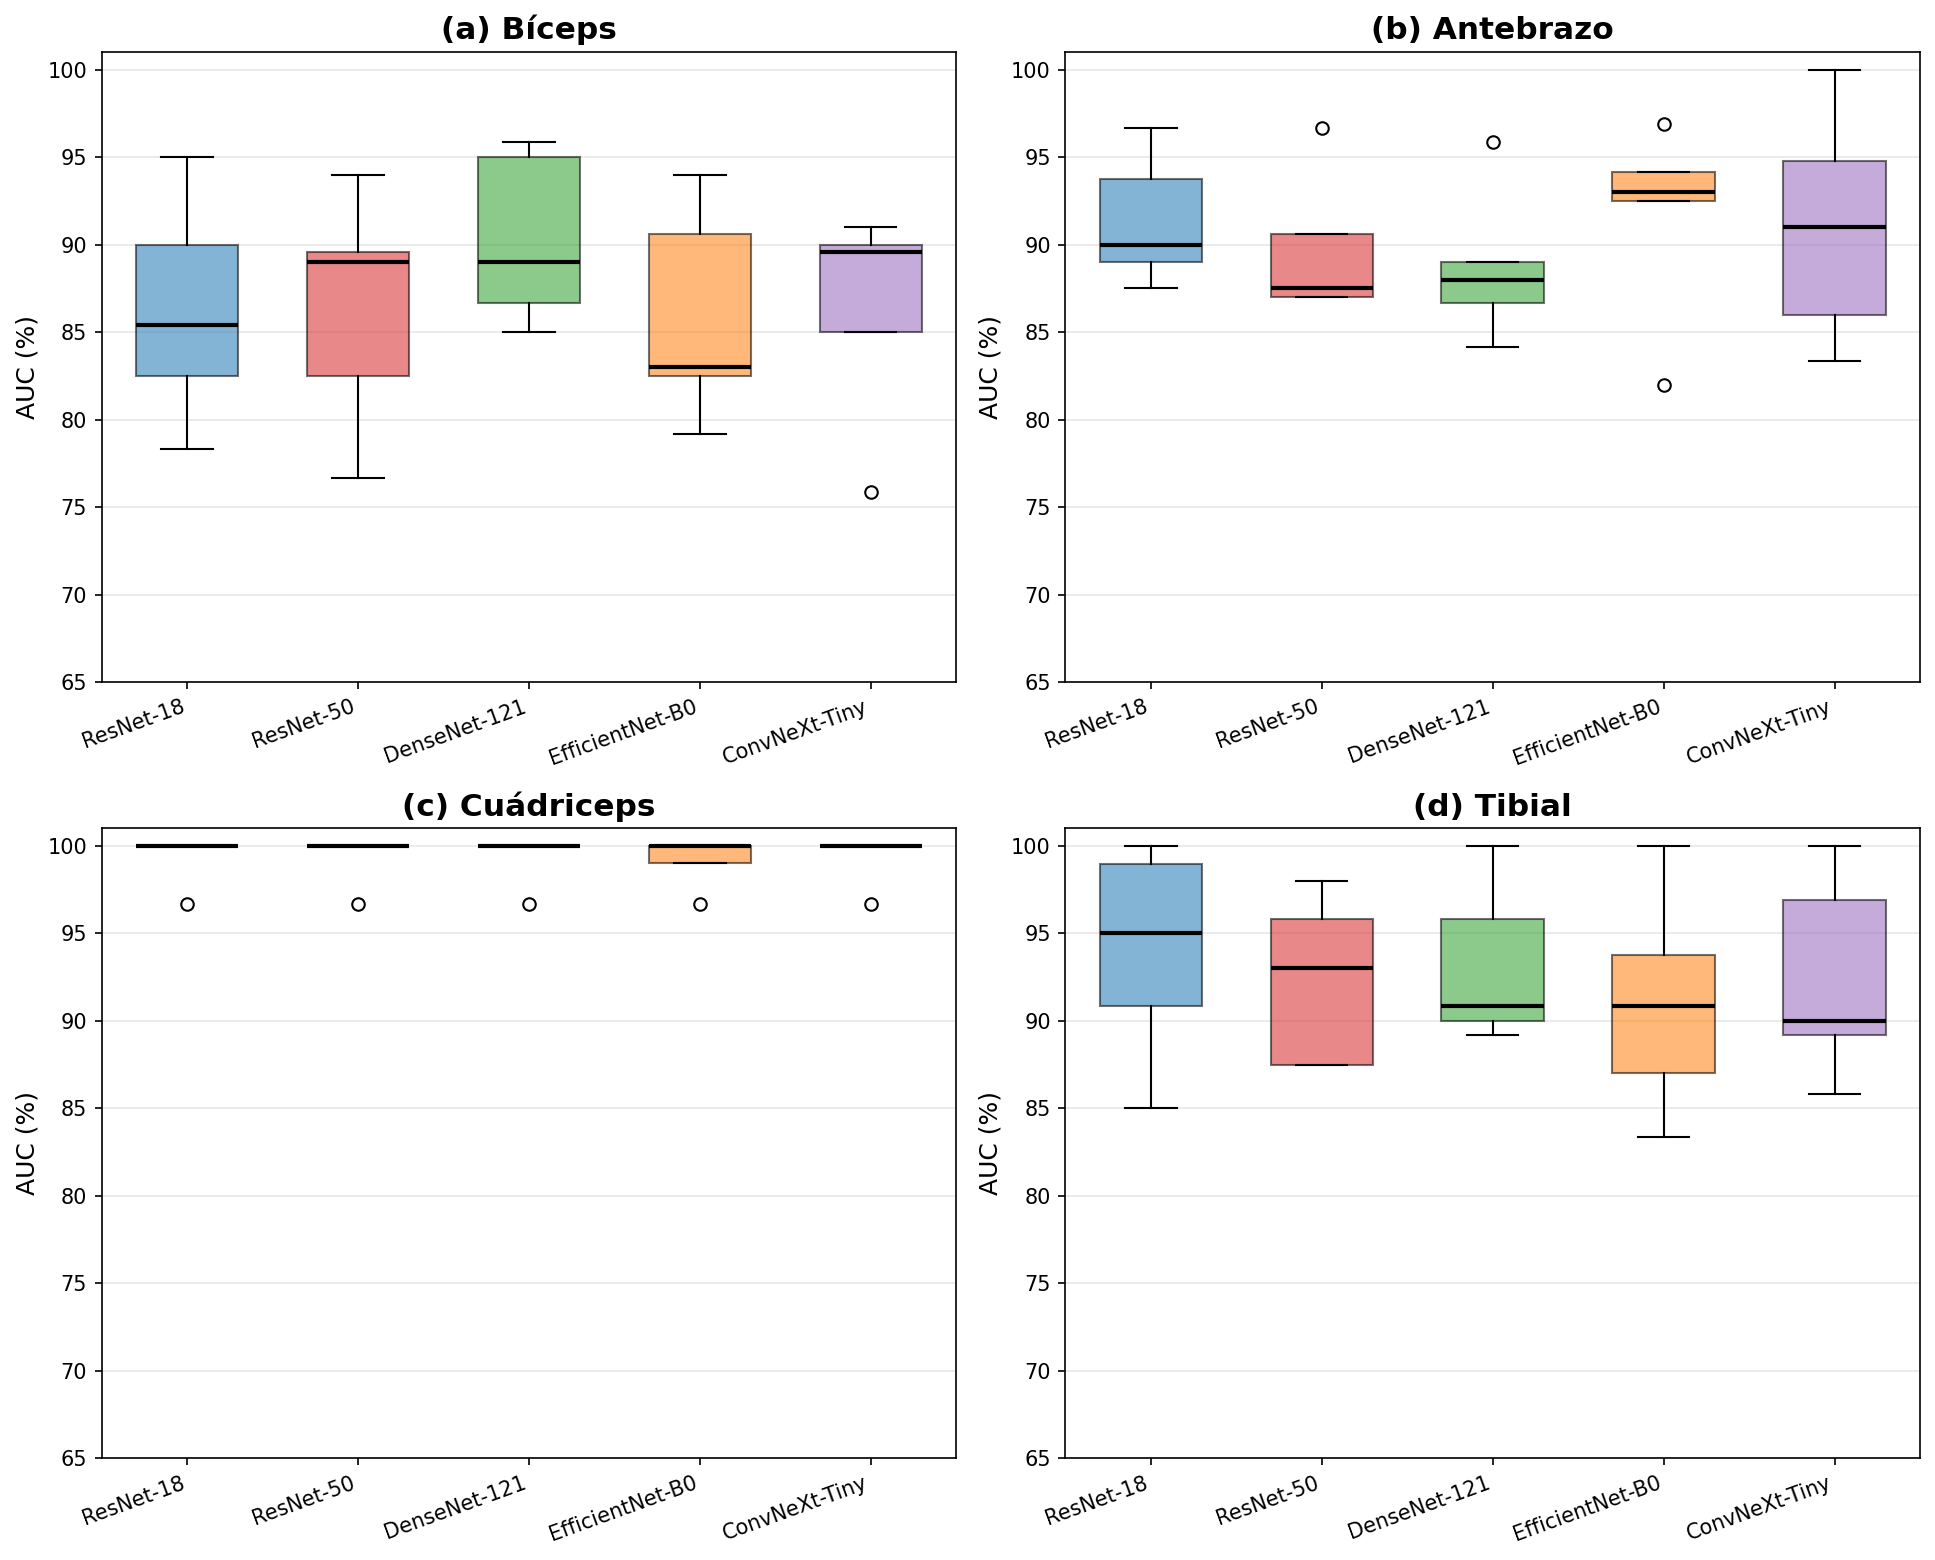
\includegraphics[width=0.92\textwidth]{images/plots/boxplot_auc_combined.png}
\caption{Distribución del AUC por \textit{fold} (5 valores) para las cinco arquitecturas en cada uno de los cuatro músculos. La altura y dispersión de cada caja resumen la consistencia del modelo: cajas más estrechas indican mayor estabilidad entre particiones. El cuádriceps presenta el patrón más consistente y elevado; el bíceps, el más disperso.}
\label{fig:boxplots-auc}
\end{figure}

Para visualizar el comportamiento de las cinco arquitecturas a lo largo de todo el rango de umbrales —no solo en la métrica resumen del AUC—, la figura~\ref{fig:roc-curves} muestra las curvas ROC obtenidas a partir de las predicciones \textit{out-of-fold} concatenadas de los cinco \textit{folds}. Cada curva agrupa las 104 predicciones (52 control + 52 ELA) de cada combinación de arquitectura y músculo.

\begin{figure}[H]
\centering
\begin{tabular}{@{}cc@{}}
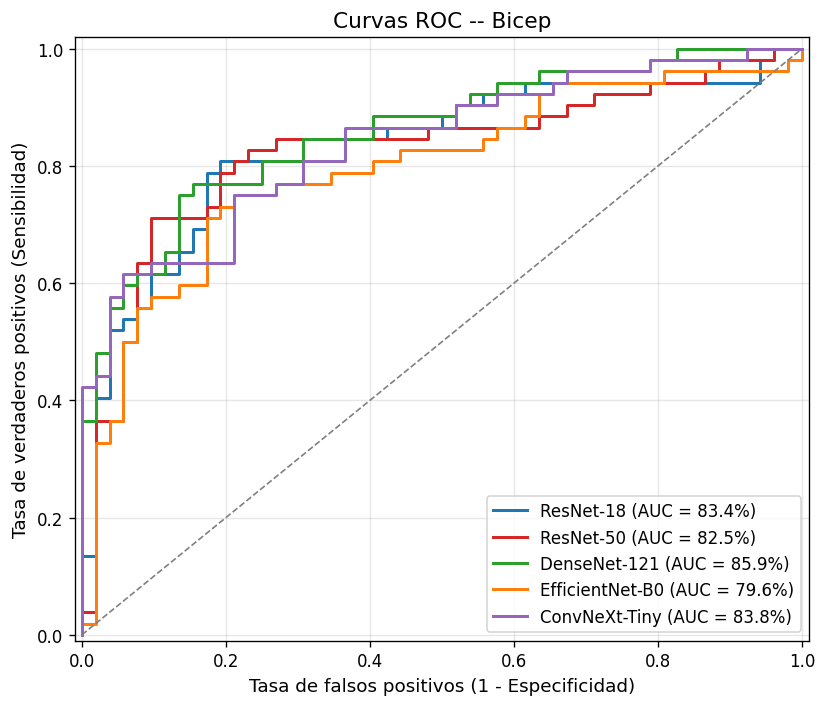
\includegraphics[width=0.45\textwidth]{images/roc/roc_bicep.png} &
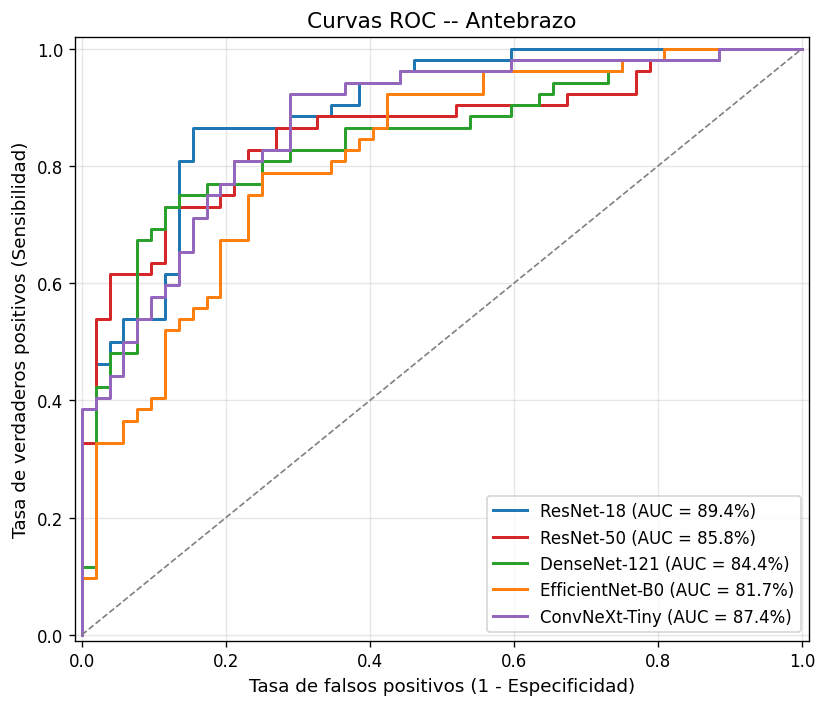
\includegraphics[width=0.45\textwidth]{images/roc/roc_antebrazo.png} \\[-2pt]
{\footnotesize (a) Bíceps} & {\footnotesize (b) Antebrazo} \\[2pt]
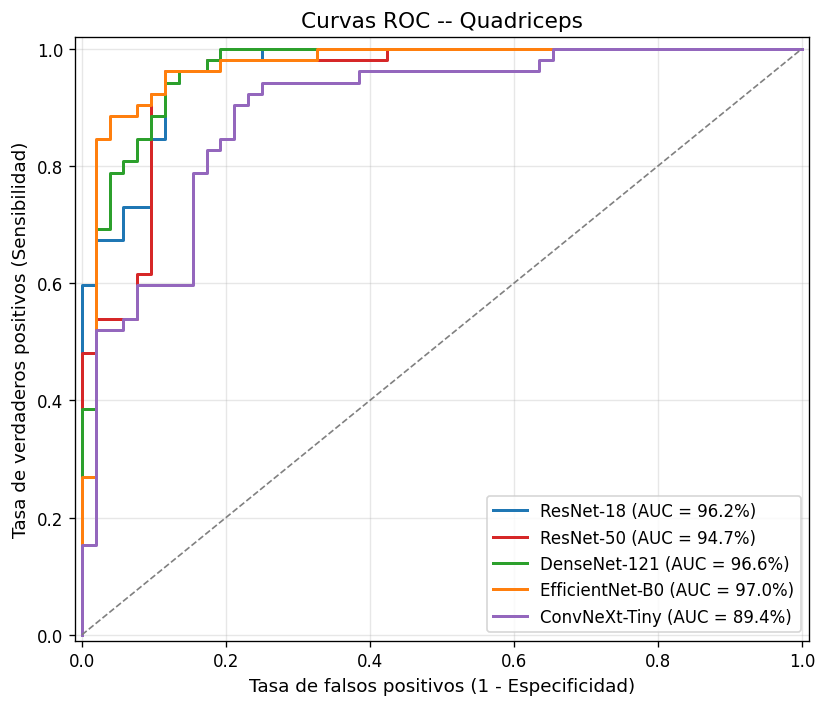
\includegraphics[width=0.45\textwidth]{images/roc/roc_quadriceps.png} &
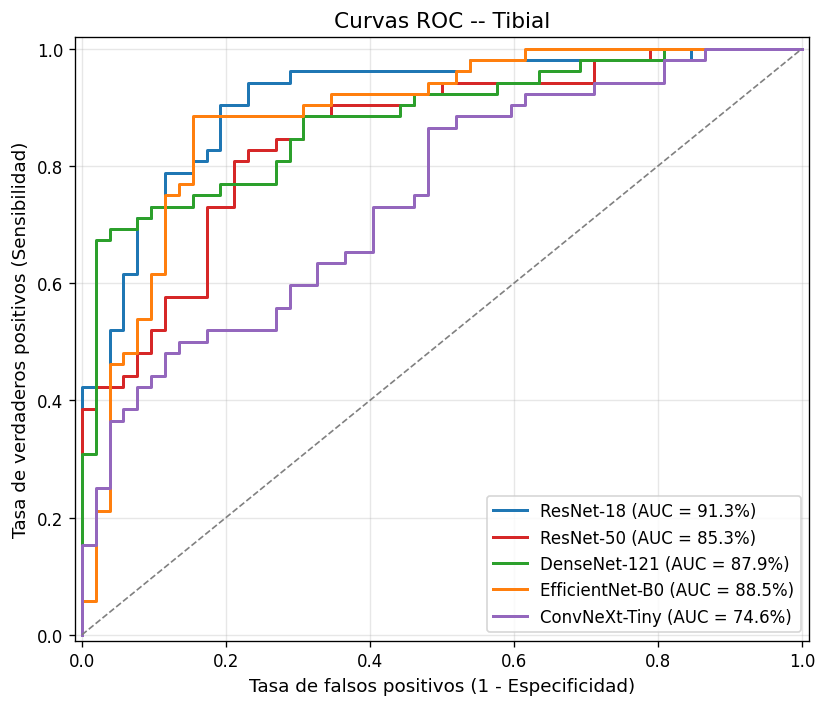
\includegraphics[width=0.45\textwidth]{images/roc/roc_tibial.png} \\[-2pt]
{\footnotesize (c) Cuádriceps} & {\footnotesize (d) Tibial} \\
\end{tabular}
\caption{Curvas ROC \textit{out-of-fold} para las cinco arquitecturas en cada uno de los cuatro músculos. Las curvas se construyen sobre las 104 predicciones concatenadas de los cinco \textit{folds}. La proximidad de las cinco curvas en cada panel ilustra gráficamente la equivalencia entre arquitecturas, y la diferencia visible entre paneles refleja la heterogeneidad entre músculos: el cuádriceps satura cerca del codo superior izquierdo, mientras que el bíceps muestra un compromiso menos favorable entre sensibilidad y especificidad.}
\label{fig:roc-curves}
\end{figure}

Las curvas confirman gráficamente las dos observaciones cuantitativas anteriores. En cuádriceps las cinco curvas se solapan casi por completo y se aproximan a la esquina superior izquierda, dejando un AUC en torno al 99\,\% y un compromiso sensibilidad-especificidad prácticamente óptimo en cualquier umbral. En bíceps, el más exigente de los cuatro, las curvas se separan más entre sí y muestran codos más suaves, lo que se traduce en una mayor dependencia del umbral elegido y justifica el peso clínico de la recalibración de Youden discutida en la sección~\ref{subsec:resultados-youden}.

\subsection{Comparación estadística entre arquitecturas}\label{subsec:resultados-stat}

Para contrastar formalmente si las diferencias de AUC observadas son estadísticamente significativas, se aplican tres pruebas complementarias a cada par de arquitecturas dentro de cada músculo: el contraste de los rangos con signo de Wilcoxon sobre los cinco valores de AUC por \textit{fold} \cite{wilcoxon1945individual}, el contraste de DeLong sobre las curvas ROC agregadas \cite{delong1988comparing} y el contraste de McNemar sobre los aciertos y fallos binarios \cite{mcnemar1947note}. Las tres pruebas son sensibles a aspectos distintos de la comparación: Wilcoxon a la dispersión de los AUC entre \textit{folds}, DeLong a la forma global de la curva ROC y McNemar a la concordancia de las predicciones binarias.

La tabla~\ref{tab:tests-resumen} sintetiza, para cada músculo, el resultado del contraste entre la arquitectura con mayor AUC medio y la segunda mejor. Con un nivel de significación $\alpha = 0{,}05$, ninguna comparación entre la mejor y la segunda mejor arquitectura resulta significativa en bíceps, antebrazo, cuádriceps ni tibial, lo que confirma la lectura inicial: las arquitecturas son, en la práctica, intercambiables a nivel de músculo individual.

\begin{table}[h!]
\centering
\caption{Contraste estadístico entre la arquitectura de mayor AUC y la segunda mejor en cada músculo. Se reportan los AUC medios (en \%) y los $p$-valores de las tres pruebas. Ningún $p$-valor es inferior a $0{,}05$.}
\label{tab:tests-resumen}
\small
\resizebox{\textwidth}{!}{%
\begin{tabular}{lllccccc}
\toprule
\textbf{Músculo} & \textbf{Mejor} & \textbf{2.ª mejor} & \textbf{AUC$_1$} & \textbf{AUC$_2$} & \textbf{$p$ Wilc.} & \textbf{$p$ DeLong} & \textbf{$p$ McNem.} \\
\midrule
Bíceps     & DenseNet-121     & ResNet-50       & 90{,}30 & 86{,}35 & 0{,}125 & 0{,}348 & 0{,}286 \\
Antebrazo  & EfficientNet-B0  & ResNet-18       & 91{,}71 & 91{,}38 & 0{,}812 & 0{,}071 & 0{,}711 \\
Cuádriceps & ResNet-18\textsuperscript{*} & EfficientNet-B0 & 99{,}33 & 99{,}13 & 1{,}000 & 0{,}746 & 0{,}424 \\
Tibial     & ResNet-18        & DenseNet-121    & 93{,}96 & 93{,}17 & 0{,}750 & 0{,}350 & 0{,}481 \\
\bottomrule
\end{tabular}%
}

\smallskip
\footnotesize{\textsuperscript{*}En cuádriceps, ResNet-18, ResNet-50, DenseNet-121 y ConvNeXt-Tiny empatan en AUC 99{,}33\,\%.}
\end{table}

El caso del cuádriceps merece un comentario adicional. Cuatro arquitecturas comparten exactamente el mismo AUC medio y la misma desviación típica entre \textit{folds}, por lo que el contraste de Wilcoxon, basado en las diferencias por \textit{fold}, no puede calcular un $p$-valor para algunas de esas parejas: la igualdad es exacta. El contraste de DeLong, que opera sobre las curvas ROC agregadas, sí detecta diferencias significativas en alguna pareja minoritaria (por ejemplo, ConvNeXt-Tiny frente a EfficientNet-B0, $p_{\text{DeLong}}=0{,}011$). Esto refleja que los modelos producen \textit{rankings} ligeramente distintos de la misma colección de imágenes, aun cuando la métrica resumen sea idéntica. La conclusión práctica es la misma: en cuádriceps el techo está tan alto que la elección de arquitectura es indiferente desde un punto de vista clínico.

El tibial es el músculo donde las pruebas pareadas detectan más diferencias entre arquitecturas. En particular, ConvNeXt-Tiny pierde frente a ResNet-18 con $p_{\text{DeLong}}=0{,}0012$ y $p_{\text{McNemar}}=0{,}0076$, y frente a DenseNet-121 con $p_{\text{DeLong}}=0{,}0004$ y $p_{\text{McNemar}}=0{,}0294$. Aunque la diferencia en AUC medio es modesta (92{,}38\,\% frente a 93{,}96\,\%), las pruebas sugieren que las arquitecturas residuales y de conexiones densas se adaptan mejor a este músculo que ConvNeXt-Tiny.

\subsection{Recalibración del umbral con el índice de Youden}\label{subsec:resultados-youden}

Las arquitecturas devuelven una probabilidad continua de pertenencia a la clase ELA, $P(\text{ELA}\mid x) \in [0,1]$. La conversión a una decisión binaria requiere fijar un umbral, y la elección por defecto ($t = 0{,}5$) no es necesariamente óptima en un escenario con clases balanceadas pero con un coste asimétrico entre falsos positivos y falsos negativos. Para cada combinación (arquitectura, músculo) se recalibra el umbral mediante el índice de Youden \cite{youden1950index}, que escoge el valor que maximiza $J = \text{Sens} + \text{Spec} - 1$ sobre la curva ROC. La tabla~\ref{tab:youden} resume el efecto de esta recalibración.

\begin{table}[h!]
\centering
\caption{Efecto de la recalibración del umbral con el índice de Youden. Se reportan sensibilidad y especificidad (en \%) con umbral fijo $t=0{,}5$ y con el umbral óptimo de Youden, así como el umbral medio resultante con su desviación típica entre \textit{folds}.}
\label{tab:youden}
\footnotesize
\begin{tabular}{llccccc}
\toprule
\textbf{Músculo} & \textbf{Arquitectura} & \textbf{Sens$_{0{,}5}$} & \textbf{Spec$_{0{,}5}$} & \textbf{Sens$_{Y}$} & \textbf{Spec$_{Y}$} & \textbf{$t_{Y}$} \\
\midrule
\multirow{5}{*}{Bíceps} & DenseNet-121      & 49{,}7 & 96{,}0 & 87{,}7 & 86{,}7 & 0{,}26 $\pm$ 0{,}18 \\
                        & ResNet-50         & 71{,}8 & 86{,}3 & 81{,}8 & 88{,}3 & 0{,}53 $\pm$ 0{,}10 \\
                        & ResNet-18         & 76{,}2 & 83{,}0 & 83{,}5 & 85{,}3 & 0{,}49 $\pm$ 0{,}23 \\
                        & ConvNeXt-Tiny     & 61{,}0 & 90{,}0 & 78{,}5 & 88{,}3 & 0{,}36 $\pm$ 0{,}15 \\
                        & EfficientNet-B0   & 63{,}3 & 82{,}7 & 85{,}3 & 81{,}0 & 0{,}43 $\pm$ 0{,}09 \\
\midrule
\multirow{5}{*}{Antebrazo} & EfficientNet-B0 & 69{,}7 & 78{,}7 & 89{,}3 & 88{,}3 & 0{,}52 $\pm$ 0{,}15 \\
                           & ConvNeXt-Tiny   & 59{,}5 & 88{,}3 & 86{,}5 & 90{,}3 & 0{,}38 $\pm$ 0{,}14 \\
                           & ResNet-50       & 78{,}5 & 78{,}7 & 83{,}3 & 92{,}7 & 0{,}56 $\pm$ 0{,}09 \\
                           & ResNet-18       & 65{,}8 & 86{,}3 & 84{,}5 & 88{,}3 & 0{,}44 $\pm$ 0{,}18 \\
                           & DenseNet-121    & 67{,}3 & 92{,}3 & 80{,}3 & 92{,}3 & 0{,}55 $\pm$ 0{,}16 \\
\midrule
\multirow{5}{*}{Cuádriceps} & ResNet-18      & 78{,}0 & 91{,}3 & 98{,}3 & 100{,}0 & 0{,}56 $\pm$ 0{,}22 \\
                            & ConvNeXt-Tiny  & 69{,}3 & 84{,}0 & 100{,}0 & 98{,}0 & 0{,}34 $\pm$ 0{,}22 \\
                            & ResNet-50      & 68{,}7 & 90{,}7 & 98{,}3 & 98{,}0 & 0{,}51 $\pm$ 0{,}11 \\
                            & DenseNet-121   & 74{,}2 & 96{,}0 & 98{,}3 & 98{,}0 & 0{,}46 $\pm$ 0{,}23 \\
                            & EfficientNet-B0& 98{,}0 & 76{,}3 & 100{,}0 & 96{,}0 & 0{,}57 $\pm$ 0{,}10 \\
\midrule
\multirow{5}{*}{Tibial} & EfficientNet-B0   & 77{,}0 & 84{,}3 & 91{,}8 & 88{,}3 & 0{,}48 $\pm$ 0{,}04 \\
                        & ResNet-18         & 78{,}8 & 86{,}3 & 88{,}3 & 92{,}3 & 0{,}48 $\pm$ 0{,}28 \\
                        & ConvNeXt-Tiny     & 51{,}7 & 83{,}7 & 98{,}3 & 80{,}7 & 0{,}38 $\pm$ 0{,}14 \\
                        & DenseNet-121      & 72{,}3 & 84{,}7 & 86{,}3 & 92{,}7 & 0{,}41 $\pm$ 0{,}26 \\
                        & ResNet-50         & 74{,}0 & 83{,}0 & 91{,}3 & 84{,}7 & 0{,}48 $\pm$ 0{,}21 \\
\bottomrule
\end{tabular}
\end{table}

El impacto de la recalibración es notable, especialmente en bíceps y cuádriceps. En bíceps, la sensibilidad de DenseNet-121 pasa del 49{,}7\,\% con umbral $0{,}5$ al 87{,}7\,\% con el umbral de Youden, manteniendo una especificidad por encima del 86\,\%; un cambio cualitativo, no marginal. En cuádriceps, varias arquitecturas alcanzan simultáneamente sensibilidades del 98--100\,\% y especificidades del 96--100\,\% tras la recalibración, lo que confirma que la limitación a umbral $0{,}5$ no era un límite de capacidad del modelo, sino una mera ineficiencia del punto de operación. Los umbrales óptimos resultantes se sitúan en su mayoría por debajo de $0{,}5$ (mediana cercana a $0{,}45$), lo que indica que las arquitecturas tienden a ser conservadoras al asignar probabilidades altas a la clase ELA en este conjunto de datos.

\subsection{Fusión a nivel paciente}\label{subsec:resultados-fusion}

El objetivo clínico último del sistema es emitir una decisión a nivel de paciente, no a nivel de imagen. Para ello se construye, para cada paciente, una probabilidad fusionada que integra la evidencia de los cuatro músculos. El procedimiento se realiza en dos pasos. En el primero, para cada paciente y cada músculo se promedian las probabilidades \textit{out-of-fold} producidas por el modelo del \textit{fold} en el que ese paciente quedó en validación; este detalle es lo que garantiza que ninguna predicción provenga de un modelo que haya visto al paciente durante el entrenamiento. En el segundo, las cuatro probabilidades resultantes se combinan mediante las tres reglas descritas en la sección~\ref{subsec:diseno}: media simple, media ponderada por el AUC del modelo en ese músculo y voto mayoritario.

Una precisión sobre el conjunto de datos: en el directorio de imágenes los sujetos control aparecen identificados como \texttt{Cnnn} en bíceps, antebrazo y cuádriceps y como \texttt{RCnnn} en tibial. Ambas convenciones se refieren al mismo individuo, lo que se confirmó con el responsable del dataset; la función \texttt{patient\_uid} en \texttt{patient\_\allowbreak level\_\allowbreak fusion.py} normaliza el identificador antes de la fusión, garantizando que las cuatro probabilidades musculares se atribuyan al mismo paciente físico.

La tabla~\ref{tab:fusion} contiene los resultados de fusión a nivel paciente para cada una de las cinco arquitecturas y las tres reglas. La métrica principal es el AUC, acompañado de su intervalo de confianza al 95\,\% obtenido por \textit{bootstrap} no paramétrico ($N=1000$) sobre los 52 pacientes. La sensibilidad, especificidad y exactitud se reportan con el umbral de Youden aplicado a la probabilidad fusionada; el voto mayoritario, al binarizar antes de la fusión, no admite un AUC fusionado y se reporta solo con sus valores de operación.

\begin{table}[h!]
\centering
\caption{Resultados de fusión a nivel paciente (52 pacientes; 26 ELA, 26 control) con las tres reglas estudiadas. Se reportan AUC, exactitud, sensibilidad y especificidad (en \%) y la matriz de confusión TP/TN/FP/FN. En negrita, el sistema final del trabajo; las últimas filas (Campeones) corresponden a la fusión de la mejor arquitectura por músculo.}
\label{tab:fusion}
\footnotesize
\begin{tabular}{llcccccc}
\toprule
\textbf{Arquitectura} & \textbf{Regla} & \textbf{AUC} & \textbf{Acc} & \textbf{Sens} & \textbf{Spec} & \textbf{TP/TN/FP/FN} \\
\midrule
\multirow{3}{*}{ResNet-18} & media simple     & 99{,}26 & 96{,}15 & 96{,}15 & 96{,}15 & 25/25/1/1 \\
                                & ponderada        & 99{,}26 & 96{,}15 & 96{,}15 & 96{,}15 & 25/25/1/1 \\
                                & voto mayoritario & -- & 90{,}38 & 80{,}77 & 100{,}00 & 21/26/0/5 \\
\midrule
\multirow{3}{*}{\textbf{ResNet-50}} & \textbf{media simple} & \textbf{98{,}67} & \textbf{96{,}15} & \textbf{100{,}00} & \textbf{92{,}31} & \textbf{26/24/2/0} \\
                                & ponderada        & 98{,}82 & 96{,}15 & 100{,}00 & 92{,}31 & 26/24/2/0 \\
                                & voto mayoritario & -- & 84{,}62 & 69{,}23 & 100{,}00 & 18/26/0/8 \\
\midrule
\multirow{3}{*}{DenseNet-121} & media simple     & 97{,}93 & 96{,}15 & 96{,}15 & 96{,}15 & 25/25/1/1 \\
                                & ponderada        & 97{,}93 & 96{,}15 & 96{,}15 & 96{,}15 & 25/25/1/1 \\
                                & voto mayoritario & -- & 78{,}85 & 61{,}54 & 96{,}15 & 16/25/1/10 \\
\midrule
\multirow{3}{*}{EfficientNet-B0} & media simple     & 98{,}22 & 96{,}15 & 96{,}15 & 96{,}15 & 25/25/1/1 \\
                                & ponderada        & 98{,}37 & 96{,}15 & 96{,}15 & 96{,}15 & 25/25/1/1 \\
                                & voto mayoritario & -- & 88{,}46 & 80{,}77 & 96{,}15 & 21/25/1/5 \\
\midrule
\multirow{3}{*}{ConvNeXt-Tiny} & media simple     & 98{,}52 & 96{,}15 & 100{,}00 & 92{,}31 & 26/24/2/0 \\
                                & ponderada        & 98{,}52 & 96{,}15 & 100{,}00 & 92{,}31 & 26/24/2/0 \\
                                & voto mayoritario & -- & 73{,}08 & 46{,}15 & 100{,}00 & 12/26/0/14 \\
\midrule
\multirow{3}{*}{Campeones\textsuperscript{\dag}} & media simple     & 99{,}11 & 94{,}23 & 100{,}00 & 88{,}46 & 26/23/3/0 \\
                                & ponderada        & 99{,}11 & 94{,}23 & 100{,}00 & 88{,}46 & 26/23/3/0 \\
                                & voto mayoritario & -- & 84{,}62 & 69{,}23 & 100{,}00 & 18/26/0/8 \\
\bottomrule
\end{tabular}

\smallskip
{\footnotesize \textsuperscript{\dag}\,Campeones: \textit{ensemble} heterogéneo que combina la mejor arquitectura por músculo (DenseNet-121 en bíceps, EfficientNet-B0 en antebrazo y ResNet-18 en cuádriceps y tibial).}
\end{table}

El sistema final del trabajo es \textbf{ResNet-50 con fusión por media simple}, que alcanza un AUC del $98{,}67$\,\% (IC95\,\% $[95{,}38;\,100{,}00]$), una exactitud del $96{,}15$\,\% (IC95\,\% $[90{,}38;\,100{,}00]$), una sensibilidad del $100$\,\% (IC95\,\% $[100{,}00;\,100{,}00]$) y una especificidad del $92{,}31$\,\% (IC95\,\% $[79{,}31;\,100{,}00]$) sobre los 52 pacientes del estudio. Las cinco arquitecturas resultan estadísticamente indistinguibles también a nivel de fusión —todos los AUC se sitúan entre 97{,}9 y 99{,}3\,\% con intervalos de confianza solapados—; entre opciones equivalentes se adopta ResNet-50 como sistema final por ser la arquitectura de referencia para \textit{transfer learning} y por ofrecer el perfil de error clínicamente más conservador, con \textbf{sensibilidad del 100\,\%} (ninguna ELA sin detectar). La matriz de confusión a nivel paciente revela dos errores, ambos falsos positivos (controles clasificados como ELA); no hay ningún falso negativo.

Varios hallazgos del proceso de fusión merecen subrayarse. En primer lugar, la media ponderada apenas mejora a la media simple: las dos reglas producen exactamente las mismas predicciones binarias en las cinco arquitecturas, y solo alteran ligeramente el AUC (a lo sumo $0{,}15$ puntos, en ResNet-50 y EfficientNet-B0). Esto se debe a que los pesos (AUC por músculo) están comprimidos en un rango estrecho —entre 86\,\% y 99\,\%— y, una vez normalizados, no priorizan ningún músculo de forma decisiva. La regla simple, al no requerir hiperparámetro alguno, es preferible. En segundo lugar, el voto mayoritario funciona muy por debajo de las dos reglas continuas: su exactitud no supera el 90{,}4\,\% en ninguna arquitectura y su sensibilidad se deteriora hasta el 46{,}2\,\% en ConvNeXt-Tiny. La explicación es metodológica: binarizar a $t=0{,}5$ por músculo antes de fusionar descarta toda la información de confianza de las probabilidades y exige el acuerdo simultáneo de al menos tres de los cuatro músculos, un criterio demasiado estricto que penaliza a los pacientes cuya señal de ELA es nítida solo en algunos músculos. La conclusión es que fusionar probabilidades es estrictamente mejor que fusionar votos.

Una estrategia alternativa que combinaría los \textit{campeones} por músculo (el modelo con mayor AUC en cada uno: DenseNet-121 en bíceps, EfficientNet-B0 en antebrazo, ResNet-18 en cuádriceps y ResNet-18 en tibial) alcanza un AUC fusionado del $99{,}11$\,\% con la regla de media simple (IC95\,\% $[97{,}00;\,100{,}00]$; últimas filas de la tabla~\ref{tab:fusion}), un valor estadísticamente indistinguible del de las arquitecturas únicas (cuyos AUC fusionados oscilan entre 97{,}9 y 99{,}3\,\%, con intervalos de confianza solapados). Mezclar arquitecturas no aporta, por tanto, una ventaja apreciable sobre emplear una sola, mientras que sí introduce complejidad operativa —cuatro arquitecturas y cuatro procedimientos de entrenamiento distintos— y, además, exhibe un perfil de error ligeramente peor (especificidad 88{,}5\,\% frente al 92{,}3\,\% del sistema ResNet-50, por tres falsos positivos frente a dos). Este resultado refuerza la elección de diseño adoptada: usar una única arquitectura entrenada por separado sobre cada músculo es preferible, por simplicidad y mantenibilidad, a un \textit{ensemble} heterogéneo de los mejores modelos por músculo.

\subsection{Comparación con la línea base clínica}\label{subsec:resultados-baseline}

La línea base de referencia para este trabajo es el sistema de análisis textural manual de Martínez-Payá y colaboradores \cite{martinezpaya2017quantitative}. La tabla~\ref{tab:baseline} resume el AUC publicado por esos autores para cada músculo, las técnicas que emplean y la comparación frente al mejor modelo de este trabajo en validación cruzada de 5 \textit{folds}.

\begin{table}[h!]
\centering
\caption{Comparación con la línea base clínica \cite{martinezpaya2017quantitative}. La columna ``Mejor arquitectura'' indica el modelo de mayor AUC en cada músculo, con su IC95\,\% \textit{bootstrap}. La columna ``Veredicto'' resume si el AUC publicado por la línea base cae dentro (equivalente) o fuera (mejora) del IC95\,\%.}
\label{tab:baseline}
\small
\resizebox{\textwidth}{!}{%
\begin{tabular}{lllcc}
\toprule
\textbf{Músculo} & \textbf{Mejor arquitectura} & \textbf{Nuestro AUC (IC95\,\%)} & \textbf{Baseline} & \textbf{Veredicto} \\
\midrule
Bíceps     & DenseNet-121     & 90{,}30 [86{,}5;\,94{,}1]  & 92{,}6 (EV+MTh)   & equivalente \\
Antebrazo  & EfficientNet-B0  & 91{,}71 [86{,}5;\,95{,}2]  & 90{,}5 (GLCM+MTh) & equivalente \\
Cuádriceps & ResNet-18        & 99{,}33 [98{,}0;\,100{,}0] & 98{,}3 (GLCM+MTh) & equivalente \\
Tibial     & ResNet-18        & 93{,}96 [89{,}0;\,98{,}6]  & 95{,}3 (EV+MTh)   & equivalente \\
\bottomrule
\end{tabular}%
}
\end{table}

En los cuatro músculos, el AUC publicado por la línea base cae dentro del intervalo de confianza al 95\,\% del mejor modelo de este trabajo. Por tanto, a nivel de músculo individual, ninguna arquitectura mejora de forma estadísticamente concluyente al análisis textural clásico. Lejos de ser un resultado negativo, esta observación es coherente con la naturaleza del problema y con la propuesta del trabajo: la aportación no es ganar al análisis textural cuando se compite músculo a músculo, sino integrar los cuatro músculos en una única decisión clínica.

La comparación adecuada del sistema completo es con la mejor combinación que la línea base puede producir a nivel paciente. El trabajo original de Martínez-Payá no propone una estrategia explícita de fusión multi-músculo a nivel paciente; reporta resultados por músculo de manera aislada. Por consiguiente, la comparación directa entre el sistema fusionado ($\text{AUC}_{\text{fusión}} = 98{,}67$\,\%) y el AUC máximo por músculo del \textit{baseline} (98{,}3\,\% en cuádriceps) no es estrictamente equivalente, pero sí ilustra la magnitud de la contribución: el sistema final mantiene un AUC cercano al 99\,\% en una clasificación a nivel paciente, mientras que el \textit{baseline} alcanza ese rango únicamente cuando se examina el músculo individualmente más informativo. La aportación fundamental del trabajo es, por tanto, la integración multi-músculo a nivel paciente con un protocolo de validación libre de fuga de información, no la mejora marginal por músculo.

\subsection{Explicabilidad: análisis cualitativo}\label{subsec:resultados-explain}

Para mitigar la naturaleza de caja negra del modelo y verificar la plausibilidad clínica de sus decisiones, se generan cuatro tipos de mapas de explicabilidad sobre el conjunto de validación: Grad-CAM \cite{selvaraju2017gradcam}, Grad-CAM guiado, mapas de saliencia \cite{simonyan2014deep} y análisis por oclusión \cite{zeiler2014visualizing}, complementado con retropropagación guiada \cite{springenberg2015striving}. La figura~\ref{fig:gradcam-mosaic} muestra una selección representativa de mapas Grad-CAM sobre los cuatro músculos, con un sujeto control y un paciente ELA para cada uno.

\begin{figure}[h!]
\centering
\begin{tabular}{cc}
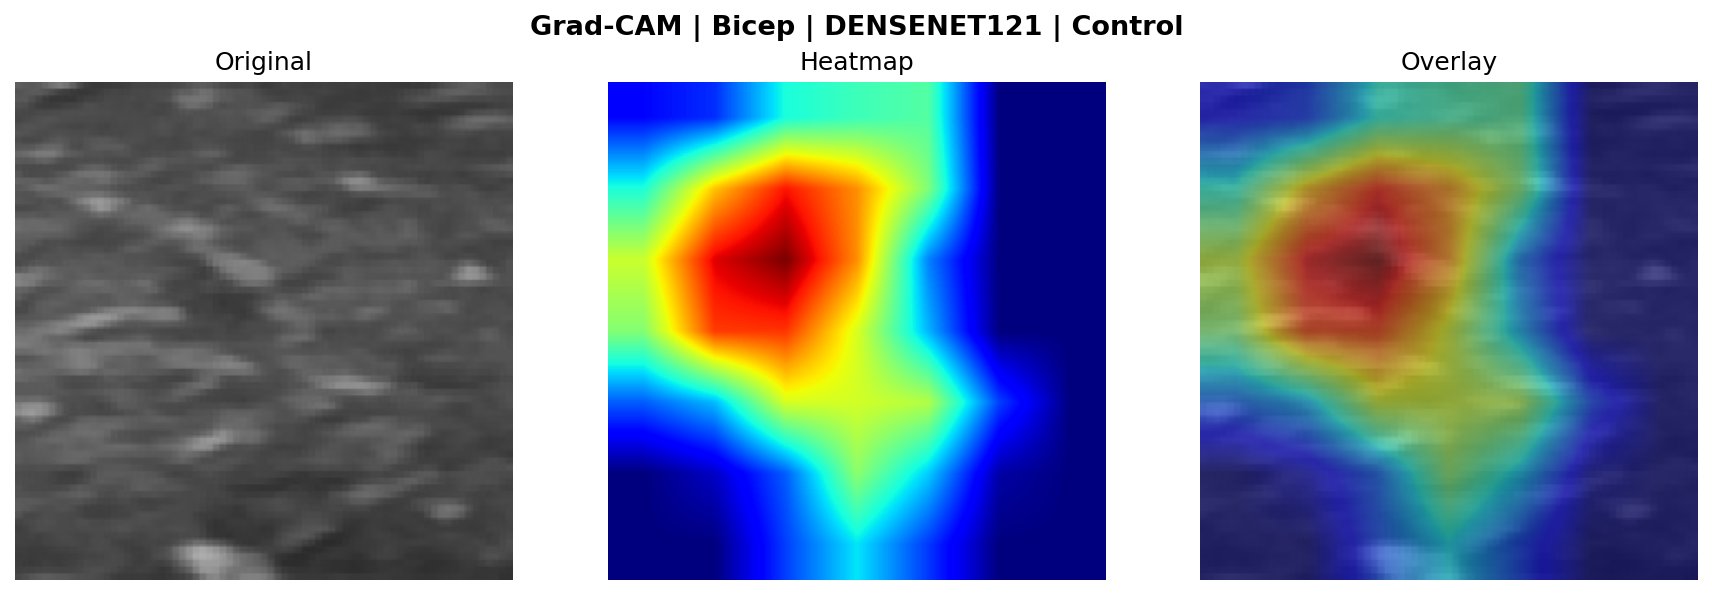
\includegraphics[width=0.35\textwidth]{images/Bicep_densenet121_Control_1.png} &
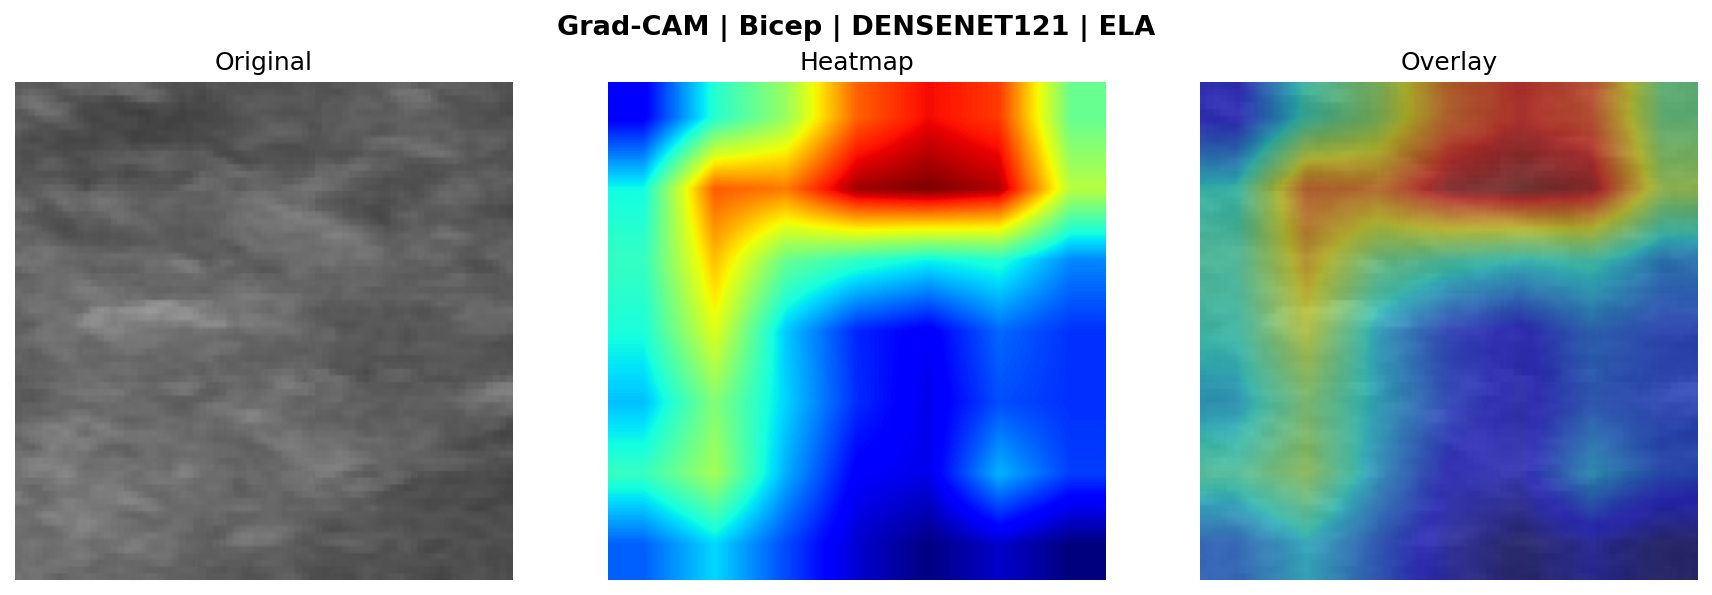
\includegraphics[width=0.35\textwidth]{images/Bicep_densenet121_ELA_3.png} \\
\multicolumn{2}{c}{\textbf{(a) Bíceps} — control (izq.) vs ELA (der.)} \\[6pt]
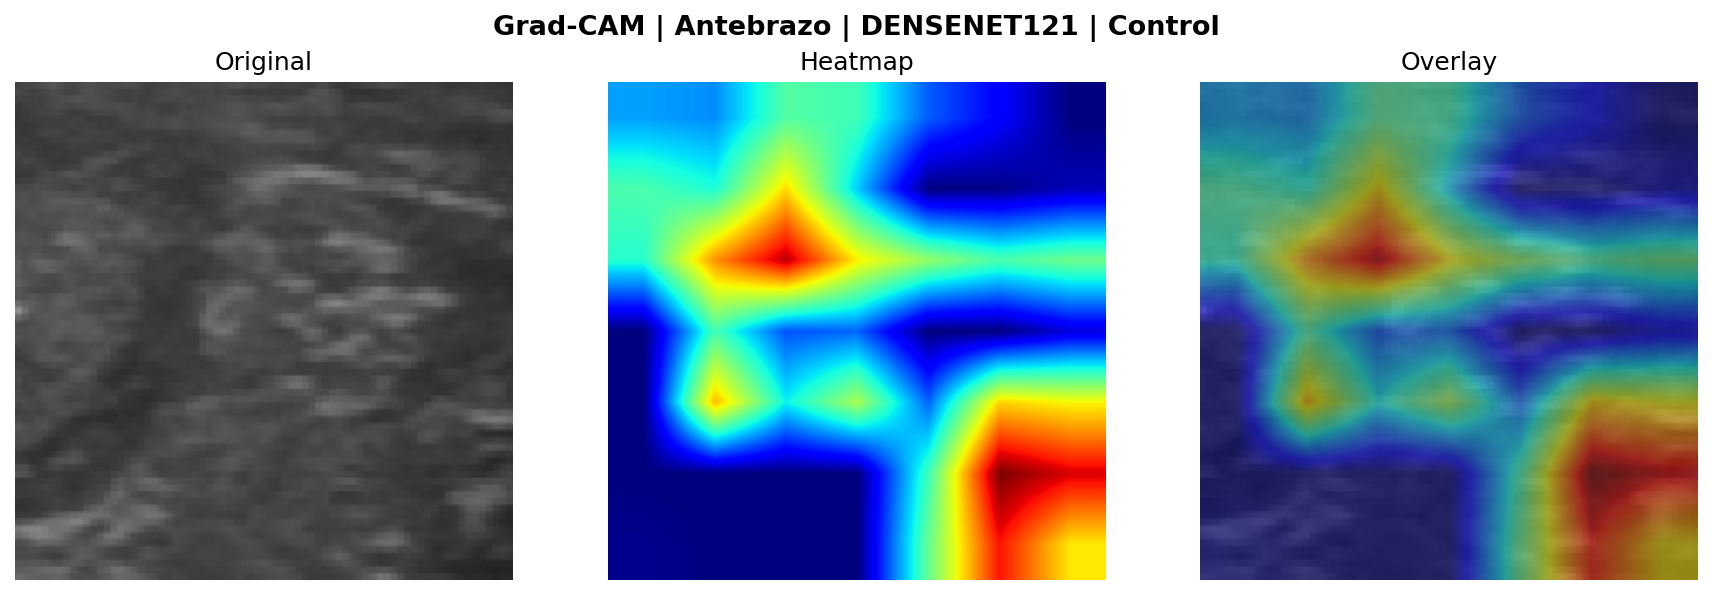
\includegraphics[width=0.35\textwidth]{images/Antebrazo_densenet121_Control_1.png} &
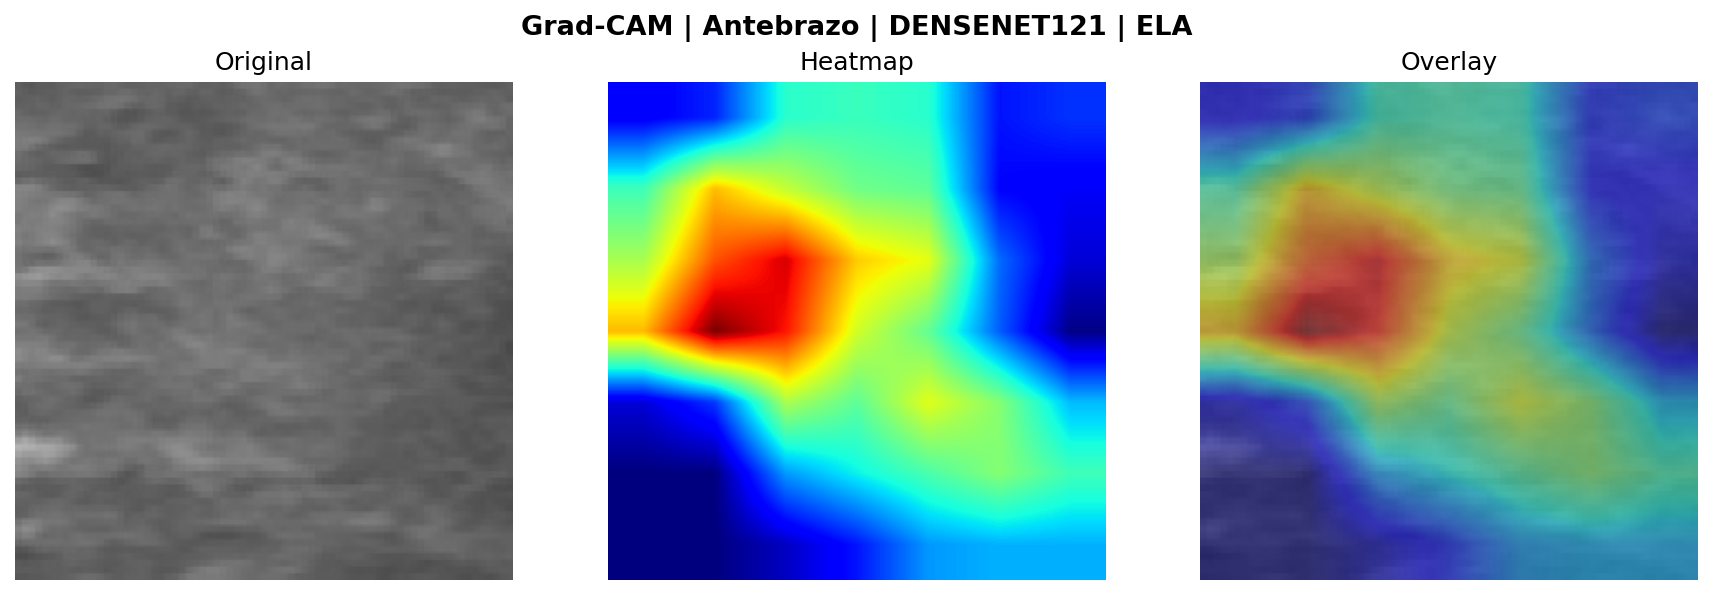
\includegraphics[width=0.35\textwidth]{images/Antebrazo_densenet121_ELA_3.png} \\
\multicolumn{2}{c}{\textbf{(b) Antebrazo} — control (izq.) vs ELA (der.)} \\[6pt]
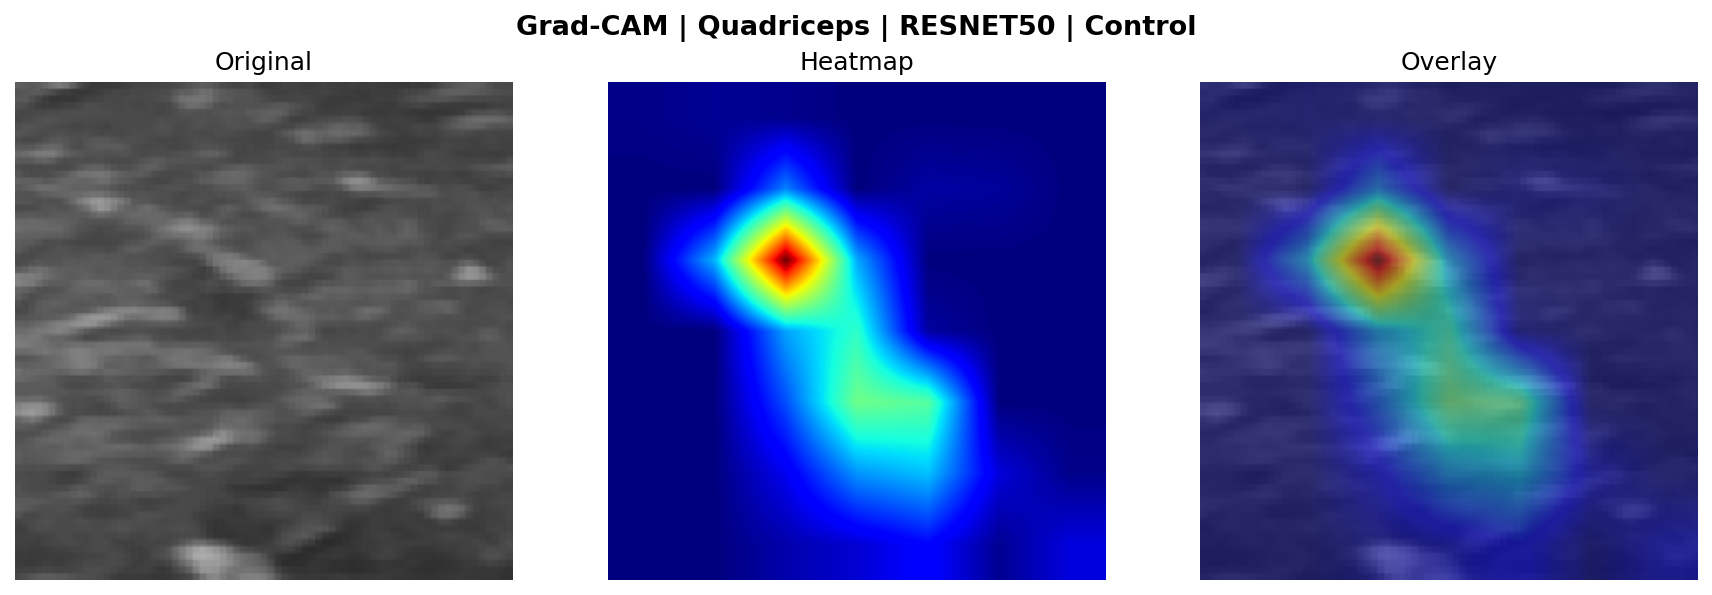
\includegraphics[width=0.35\textwidth]{images/Quadriceps_resnet50_Control_1.png} &
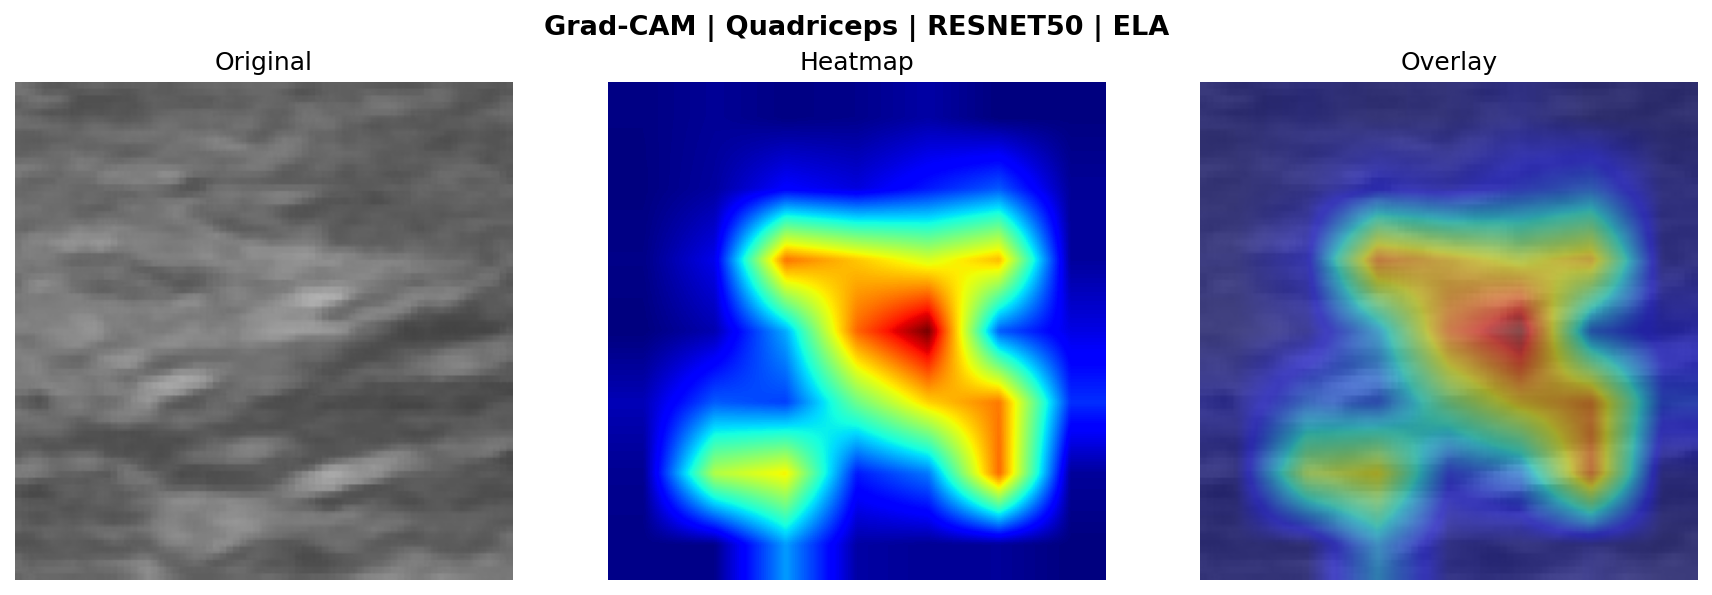
\includegraphics[width=0.35\textwidth]{images/Quadriceps_resnet50_ELA_3.png} \\
\multicolumn{2}{c}{\textbf{(c) Cuádriceps} — control (izq.) vs ELA (der.)} \\[6pt]
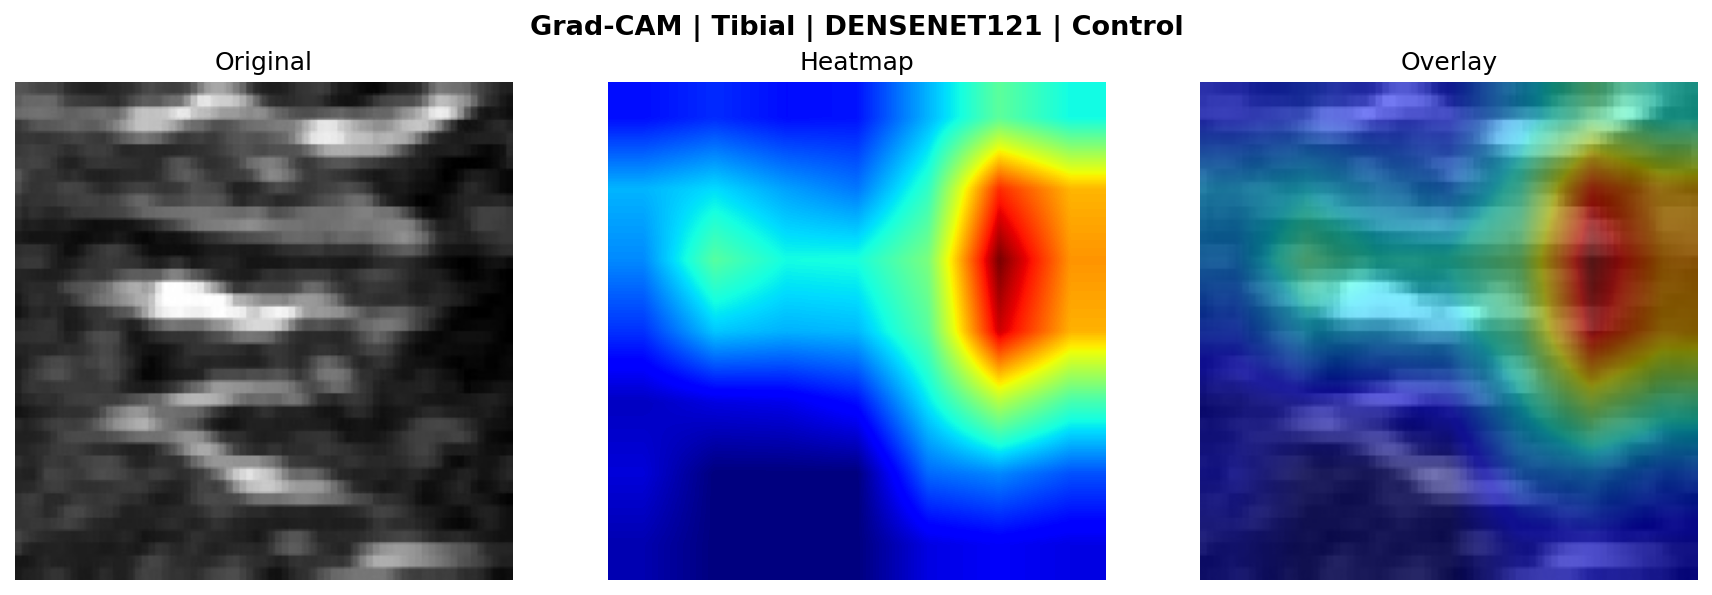
\includegraphics[width=0.35\textwidth]{images/Tibial_densenet121_Control_1.png} &
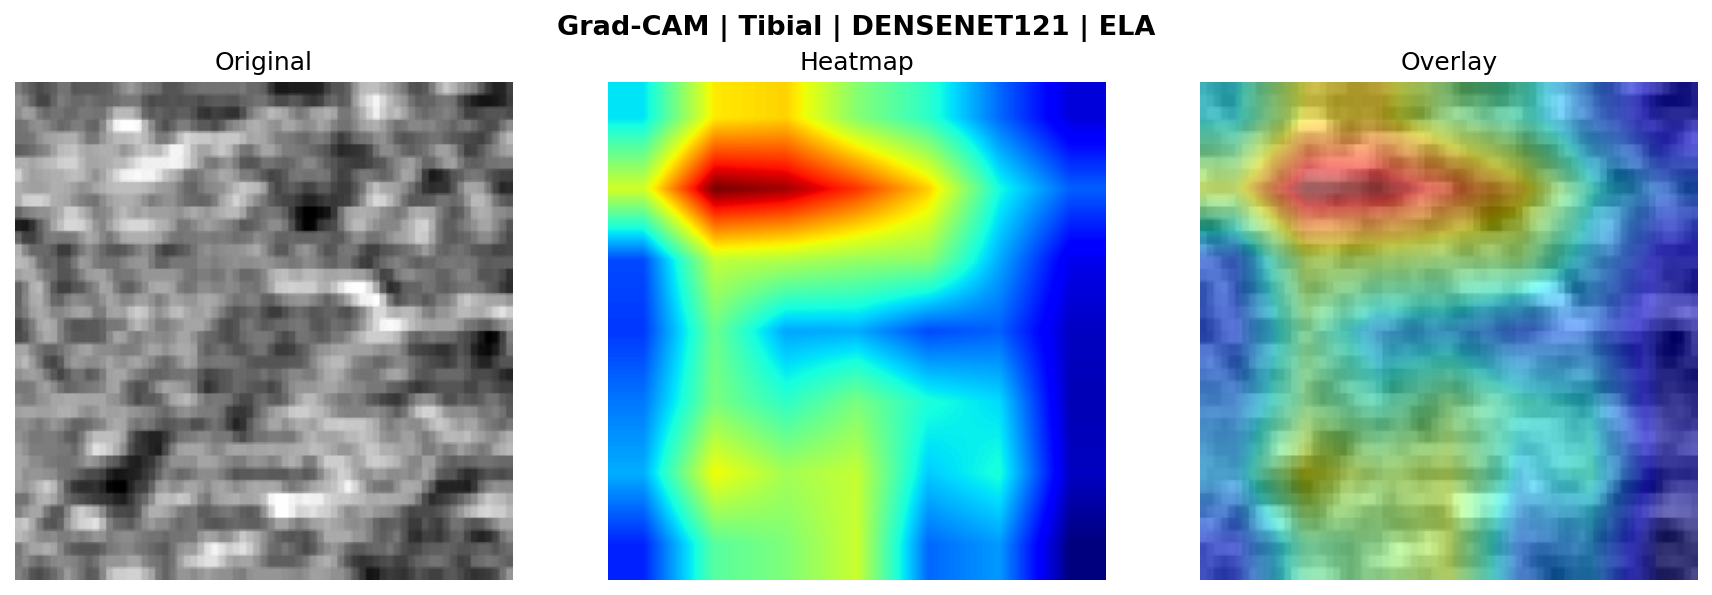
\includegraphics[width=0.35\textwidth]{images/Tibial_densenet121_ELA_3.png} \\
\multicolumn{2}{c}{\textbf{(d) Tibial} — control (izq.) vs ELA (der.)} \\
\end{tabular}
\caption{Mapas Grad-CAM sobre los cuatro músculos analizados. Para cada músculo se muestra un sujeto control (izquierda) y un paciente ELA (derecha). Las activaciones se concentran sobre el parénquima muscular y evitan los bordes de la imagen y los marcadores del ecógrafo, lo que indica que el modelo se apoya en regiones clínicamente plausibles para emitir su predicción.}
\label{fig:gradcam-mosaic}
\end{figure}

El análisis cualitativo aporta tres conclusiones principales. En primer lugar, las activaciones de mayor magnitud se localizan sobre el tejido muscular y no sobre artefactos externos como los bordes negros, las inscripciones del ecógrafo o las marcas de medición; este hallazgo es necesario para considerar al modelo confiable desde un punto de vista clínico. En segundo lugar, los mapas de los pacientes con ELA muestran activaciones más extensas y heterogéneas que las de los controles, una observación cualitativamente consistente con la fisiopatología de la enfermedad —la sustitución de tejido contráctil por tejido fibroadiposo aumenta la ecointensidad y la heterogeneidad textural— y, por tanto, con la literatura clínica previa \cite{pillen2008muscle,martinezpaya2017quantitative}. En tercer lugar, los mapas de las cuatro técnicas (Grad-CAM, Grad-CAM guiado, saliencia y oclusión) coinciden cualitativamente entre sí en la localización de las regiones discriminantes, lo que refuerza la robustez de la interpretación: no se trata de un artefacto particular de un método de explicabilidad concreto, sino de una propiedad reproducible del modelo.

Es importante puntualizar dos limitaciones intrínsecas de este tipo de análisis para el problema concreto que se aborda. La primera es de \textbf{resolución}: la última capa convolucional de ResNet-50 sobre una entrada de $224\times 224$ píxeles tiene una resolución espacial de $7\times 7$, que es la rejilla nativa sobre la que Grad-CAM produce sus mapas antes de reescalarlos por interpolación bilineal al tamaño original. Esta resolución intrínseca limita el detalle anatómico que pueden mostrar los focos de calor y explica el aspecto «suave» o difuso característico de las activaciones que se observan en la figura~\ref{fig:gradcam-mosaic}. La segunda limitación es de \textbf{naturaleza del problema}: Grad-CAM, y en general las técnicas de explicabilidad basadas en localización, responden a la pregunta de \textit{dónde} mira el modelo, no a la de \textit{qué} ve en la región atendida. En un problema de clasificación textural como el aquí planteado, en el que la información discriminante reside en el patrón fino del parénquima muscular (granulado, fibrosis, distribución de la ecointensidad) y no en la posición espacial del músculo en la imagen, es esperable que las regiones atendidas para ELA y control compartan ubicaciones similares —el centro del músculo— aunque la decisión final difiera. Precisamente por esta limitación se emplean cuatro técnicas complementarias —Grad-CAM, Grad-CAM guiado, mapas de saliencia y análisis por oclusión— que sondean el modelo desde mecanismos distintos y, cuando coinciden en señalar las mismas regiones, refuerzan la robustez de la interpretación más allá de lo que cualquiera de ellas podría sostener por separado.

Los mapas de explicabilidad son, en última instancia, una herramienta de verificación cualitativa, no una prueba formal de causalidad. Demuestran que el modelo se apoya en regiones clínicamente plausibles, no que sus decisiones individuales sean clínicamente correctas. Una validación clínica completa requeriría el contraste con un radiólogo experto sobre cada caso, un trabajo que excede el alcance de este Trabajo Fin de Grado pero que se identifica como línea de investigación futura en el capítulo~\ref{sec:conclusion}.

\subsection{Síntesis del capítulo}\label{subsec:resultados-resumen}

A nivel de músculo, las cinco arquitecturas estudiadas son estadísticamente equivalentes entre sí y, simultáneamente, equivalentes a la línea base clínica de Martínez-Payá: ningún contraste pareado entre la mejor y la segunda mejor arquitectura alcanza significación en ninguno de los cuatro músculos, y todos los AUC publicados por la línea base caen dentro de los intervalos de confianza de los modelos de este trabajo. La recalibración del umbral mediante el índice de Youden mejora la sensibilidad de forma sustancial sin sacrificar especificidad, hasta el punto de que en cuádriceps varias arquitecturas alcanzan simultáneamente sensibilidad y especificidad próximas al 100\,\%.

El aporte central del trabajo aparece al integrar los cuatro músculos en una única decisión por paciente. La fusión por media simple de las probabilidades \textit{out-of-fold} de ResNet-50 produce el sistema final: AUC del 98{,}67\,\%, exactitud del 96{,}15\,\%, sensibilidad del 100\,\% y especificidad del 92{,}31\,\% sobre los 52 pacientes, con dos errores de clasificación, ambos falsos positivos y ninguna ELA sin detectar. La regla ponderada por AUC no aporta mejora apreciable sobre la media simple, y el voto mayoritario se descarta por su deterioro sistemático de la sensibilidad. Una estrategia alternativa que mezcle arquitecturas distintas (campeones por músculo) obtiene un rendimiento equivalente al de la arquitectura única, por lo que esta última se prefiere por su mayor simplicidad operativa. Los mapas de explicabilidad confirman que la predicción se sustenta sobre el parénquima muscular, en regiones clínicamente plausibles. El siguiente capítulo discute las implicaciones de estos resultados y las líneas de trabajo futuro.

\newpage

%%%%%%%%%%%%%%%%%%%%%%%%%%%%%%%%%%%%%%%%%%%%%%%%%%%%%%%%
%%%% Conclusiones %%%%%%%%%%%%%%%%%%%%%%%%%%%%%%%%%%%%%%%
%%%%%%%%%%%%%%%%%%%%%%%%%%%%%%%%%%%%%%%%%%%%%%%%%%%%%%%%
\section{Conclusiones y Trabajo Futuro}\label{sec:conclusion}

Este capítulo cierra la memoria evaluando el grado de cumplimiento de los objetivos planteados en el capítulo~1, resumiendo las aportaciones técnicas y metodológicas del sistema, exponiendo las limitaciones del trabajo y trazando las líneas de investigación que de forma natural lo prolongan.

\subsection{Cumplimiento de los objetivos}\label{subsec:conc-objetivos}

El objetivo principal del trabajo —diseñar, implementar y validar un sistema de soporte al diagnóstico de la ELA basado en redes neuronales convolucionales aplicadas a ecografía muscular y operando a nivel de paciente— se considera \textbf{alcanzado}. El sistema final, ResNet-50 entrenado de forma independiente sobre cada uno de los cuatro músculos y fusionado mediante la media simple de las probabilidades \textit{out-of-fold}, alcanza sobre los 52 pacientes del estudio un AUC del 98{,}67\,\%, una exactitud del 96{,}15\,\%, una sensibilidad del 100\,\% y una especificidad del 92{,}31\,\%, con dos errores de clasificación (ambos falsos positivos). Cada objetivo específico planteado en el capítulo~1 se ha cubierto del siguiente modo:

\begin{itemize}
    \item Se han entrenado y comparado las cinco arquitecturas previstas (ResNet-18, ResNet-50, DenseNet-121, EfficientNet-B0 y ConvNeXt-Tiny) sobre los cuatro músculos del estudio, con un total de 100 modelos entrenados ($5\times 4\times 5$ \textit{folds}), reportados en la sección~\ref{subsec:resultados-por-musculo}.
    \item Se ha garantizado la integridad metodológica de la validación mediante \texttt{Stratified\allowbreak Group\allowbreak KFold} con agrupación por sujeto. Una aserción explícita en \texttt{dataset.py} verifica en cada \textit{fold} la ausencia de solapamiento entre los conjuntos de entrenamiento y validación, salvaguarda frente a la fuga de información descrita por la literatura \cite{saeb2017need,roberts2021common}.
    \item La incertidumbre se ha cuantificado con tres herramientas complementarias: intervalos de confianza al 95\,\% por aproximación de la t de Student y por \textit{bootstrap} sobre los AUC por \textit{fold} (tabla~\ref{tab:auc-ci}), recalibración del umbral mediante el índice de Youden \cite{youden1950index} (tabla~\ref{tab:youden}) y contrastes de hipótesis pareados entre arquitecturas (Wilcoxon, DeLong y McNemar, tabla~\ref{tab:tests-resumen}).
    \item Se ha diseñado y validado una estrategia de fusión a nivel paciente con tres reglas —media simple, media ponderada por AUC y voto mayoritario— reportada en la tabla~\ref{tab:fusion}. La media simple resultó la mejor opción por su equilibrio entre sensibilidad y especificidad, y la fusión con una única arquitectura superó a la mezcla de campeones por músculo, una conclusión metodológica relevante.
    \item Se han generado mapas de explicabilidad (Grad-CAM, Grad-CAM guiado, mapas de saliencia y análisis por oclusión) sobre el sistema final (sección~\ref{subsec:resultados-explain}), que confirman que las activaciones del modelo se concentran sobre el parénquima muscular y no sobre artefactos de la imagen.
    \item La comparación con la línea base clínica de Martínez-Payá \cite{martinezpaya2017quantitative} se ha realizado a nivel músculo mediante el criterio del intervalo de confianza (tabla~\ref{tab:baseline}), arrojando un veredicto de equivalencia en los cuatro músculos, y se ha discutido cualitativamente la contribución diferencial de la fusión multi-músculo, que el trabajo base no contempla.
\end{itemize}

\subsection{Conclusiones principales}\label{subsec:conc-principales}

Del trabajo se desprenden cuatro conclusiones de fondo.

En primer lugar, a nivel de músculo individual, \textbf{las arquitecturas convolucionales modernas son intercambiables entre sí y estadísticamente equivalentes a la línea base de análisis textural clásico}. Ninguna comparación pareada entre la mejor y la segunda mejor arquitectura alcanza significación en bíceps, antebrazo, cuádriceps ni tibial, y todos los AUC publicados por Martínez-Payá caen dentro de los intervalos de confianza al 95\,\% de los modelos de este trabajo. Lejos de invalidar el enfoque, este resultado lo enmarca con precisión: el aprendizaje profundo no aporta una mejora marginal por músculo, sino que sustituye un descriptor diseñado a mano por uno aprendido y libera la metodología para incorporar etapas posteriores —en este caso, la fusión— que el análisis textural clásico no soporta de forma natural.

En segundo lugar, \textbf{la integración multi-músculo a nivel paciente es la aportación fundamental del trabajo}. La fusión por media simple de las probabilidades de los cuatro músculos eleva el rendimiento desde un rango del 86--99\,\% por músculo —con varianza apreciable— a un AUC del 98{,}67\,\% a nivel paciente, con solo dos errores sobre 52 sujetos (ambos falsos positivos; ninguna ELA sin detectar). Este salto no proviene de mejorar el clasificador por imagen, sino de utilizar de forma estadísticamente honesta toda la evidencia disponible para cada paciente: una observación coherente con la naturaleza clínica del problema, en el que el especialista nunca emite un diagnóstico a partir de un solo músculo.

En tercer lugar, \textbf{el diseño con una única arquitectura entrenada de forma independiente por músculo es preferible, por simplicidad operativa, a un \textit{ensemble} heterogéneo de los mejores modelos por músculo}. La fusión de los campeones alcanza un AUC del 99{,}11\,\%, estadísticamente indistinguible del de las arquitecturas únicas (cuyos AUC fusionados oscilan entre 97{,}9 y 99{,}3\,\% con intervalos de confianza solapados). Mezclar arquitecturas no aporta, por tanto, una ventaja apreciable de rendimiento y sí añade complejidad. Esta observación tiene implicaciones prácticas: el sistema final es operativamente más simple —un único tipo de red, un único procedimiento de entrenamiento— y, por tanto, más mantenible.

En cuarto lugar, \textbf{la transparencia metodológica es indistinguible del rendimiento medido}. La validación cruzada agrupada por paciente, la recalibración del umbral mediante el índice de Youden, los intervalos de confianza por \textit{bootstrap} y los contrastes pareados han permitido reportar resultados que son simultáneamente altos y honestos. Esta exigencia es la salvaguarda frente al fenómeno, recurrentemente documentado en la literatura \cite{roberts2021common}, de modelos con métricas espectaculares sobre el conjunto de validación que no generalizan más allá.

\subsection{Limitaciones del trabajo}\label{subsec:conc-limitaciones}

Una evaluación responsable de los resultados anteriores debe ponerlos en contexto frente a las limitaciones del trabajo, que son las propias de un estudio piloto con un conjunto clínico reducido.

La limitación más relevante es el \textbf{tamaño y la procedencia única del conjunto de datos}. Los 52 pacientes proceden de un mismo centro y han sido adquiridos con un protocolo y un equipo homogéneos. Aunque la validación cruzada agrupada por sujeto previene la fuga de información dentro de este conjunto, no aporta evidencia sobre la generalización a otras instituciones, otros ecógrafos u otras poblaciones. Un AUC del 98{,}67\,\% sobre 52 pacientes es una estimación con un intervalo de confianza ancho (límite inferior del IC95\,\% \textit{bootstrap} en $95{,}38$\,\%) y debe interpretarse como tal.

La segunda limitación es la \textbf{ausencia de validación externa con una cohorte independiente}. El conjunto disponible se ha agotado en la propia validación cruzada, sin reservar una porción para evaluación final ciega; esa decisión de diseño se justifica por el tamaño muestral, pero implica que el sistema no ha sido contrastado nunca contra datos que no hayan participado en la elección de hiperparámetros y arquitectura.

La tercera limitación es la \textbf{ausencia de contraste con un radiólogo experto}. Los mapas de explicabilidad demuestran que el modelo se apoya en regiones plausibles, pero esta es una verificación cualitativa: no se ha llevado a cabo una concordancia paciente a paciente entre las decisiones del sistema y el juicio independiente de un especialista, contraste que sería necesario antes de cualquier integración clínica.

Finalmente, el sistema produce una probabilidad y una decisión binaria, pero \textbf{no proporciona una estimación de incertidumbre por paciente individual}. Para un uso clínico responsable sería deseable acompañar cada predicción de un intervalo de confianza propio del paciente, que distinga las decisiones rotundas de las situadas cerca del umbral.

\subsection{Líneas de trabajo futuro}\label{subsec:conc-futuro}

Las limitaciones anteriores sugieren las líneas naturales de continuación del proyecto.

\textbf{Validación externa con una cohorte independiente.} La primera prioridad metodológica es contrastar el sistema con un conjunto de pacientes adquiridos en otra institución y con otro equipo de ecografía. Durante el desarrollo de este trabajo se ha identificado una cohorte adicional compatible con la metodología propuesta \cite{aljaro2026quantitative}; aplicar el modelo ya entrenado a esos datos —sin reentrenar— constituiría la prueba de generalización más exigente y es el siguiente paso inmediato del proyecto.

\textbf{Calibración y cuantificación de la incertidumbre.} Las probabilidades emitidas por el modelo se han recalibrado mediante el índice de Youden a nivel de umbral, pero no se han calibrado a nivel de distribución; técnicas como la regresión isotónica o el escalado de Platt producirían probabilidades cuya magnitud reflejara la confianza real del modelo, requisito necesario para integrarlo con otras fuentes de información clínica. De forma complementaria, métodos como \textit{deep ensembles} o \textit{Monte Carlo dropout} permitirían acompañar cada decisión de una estimación de incertidumbre por paciente, distinguir los casos rotundos de los marginales y, en último término, recomendar la derivación de los casos dudosos a una segunda lectura humana.

\textbf{Extensión a monitorización longitudinal.} Trabajos previos del grupo de Martínez-Payá han documentado que los descriptores texturales reflejan la progresión de la enfermedad a lo largo del tiempo \cite{martinezpaya2018monitoring}. Adaptar la arquitectura propuesta a una entrada longitudinal —varias adquisiciones por paciente a lo largo de meses— permitiría pasar del diagnóstico al seguimiento, una aplicación clínica de gran valor en una enfermedad como la ELA.

\textbf{Integración clínica.} Más allá del modelo, la incorporación efectiva del sistema a un flujo asistencial requiere un protocolo de operación definido —umbrales aprobados, criterios de decisión asistida y no automática—, una interfaz integrada con el ecógrafo o el sistema PACS y, sobre todo, un estudio de concordancia con radiólogos sobre una cohorte suficientemente amplia.

\subsection{Reflexión final}\label{subsec:conc-cierre}

El trabajo demuestra que es posible aplicar aprendizaje profundo a la detección de ELA a partir de ecografía muscular alcanzando un rendimiento clínicamente operativo y, simultáneamente, sostenido por un protocolo de validación riguroso. La aportación no reside únicamente en los números —que son altos, pero acotados por las limitaciones de un estudio piloto—, sino en la combinación de tres elementos: la sustitución del análisis textural manual por descriptores aprendidos, la integración multi-músculo a nivel paciente y el control explícito de la fuga de información por sujeto. Cualquiera de los tres sin los otros dos produciría un sistema más débil. Tomados conjuntamente, definen una metodología reproducible y extensible que constituye el legado técnico de este Trabajo Fin de Grado y la base sobre la que se asientan las líneas de trabajo futuro identificadas.

\newpage

%%%%%%%%%%%%%%%%%%%%%%%%%%%%%%%%%%%%%%%%%%%%%%%%%%%%%%%%
%%%% Referencias %%%%%%%%%%%%%%%%%%%%%%%%%%%%%%%%%%%%%%%
%%%%%%%%%%%%%%%%%%%%%%%%%%%%%%%%%%%%%%%%%%%%%%%%%%%%%%%%
\section{Bibliograf\'ia} \label{sec:bibliography}

\printbibliography[heading=none]

\end{refsection}
\newpage

%%%%%%%%%%%%%%%%%%%%%%%%%%%%%%%%%%%%%%%%%%%%%%%%%%%%%%%%
%%%% Anexos %%%%%%%%%%%%%%%%%%%%%%%%%%%%%%%%%%%%%%%%%%%%
%%%%%%%%%%%%%%%%%%%%%%%%%%%%%%%%%%%%%%%%%%%%%%%%%%%%%%%%
\appendix
\section{Material complementario}\label{sec:anexo-a}

Este anexo recoge información complementaria al cuerpo principal de la memoria: la configuración exacta del entrenamiento, la tabla completa de las comparaciones estadísticas pareadas entre arquitecturas y los mapas de explicabilidad generados sobre el sistema final.

\subsection{Configuración completa del entrenamiento}\label{subsec:anexo-hiperparams}

La tabla~\ref{tab:hiperparams} reúne todos los hiperparámetros, semillas y rutas relevantes del experimento principal, tal y como aparecen en \texttt{src/config.py} y en los módulos de entrenamiento (\texttt{train\_\allowbreak kfold.py}) y fusión (\texttt{patient\_\allowbreak level\_\allowbreak fusion.py}). Su propósito es permitir la reproducción exacta del experimento.

\begin{table}[H]
\centering
\caption{Hiperparámetros y configuración del experimento principal del trabajo.}
\label{tab:hiperparams}
\small
\resizebox{\textwidth}{!}{%
\begin{tabular}{ll}
\toprule
\textbf{Parámetro} & \textbf{Valor} \\
\midrule
Semilla de aleatoriedad & 42 (propagada a Python, NumPy, PyTorch y scikit-learn) \\
Tamaño de imagen & $224 \times 224$ píxeles, 3 canales (RGB) \\
Normalización & Media $[0{,}485, 0{,}456, 0{,}406]$, std $[0{,}229, 0{,}224, 0{,}225]$ (ImageNet) \\
Aumento entren. & Flip h. $p=0{,}5$, flip v. $p=0{,}2$, rotación $\pm 10^{\circ}$, color jitter $\pm 0{,}2$, traslación $\pm 5$\,\% \\
Aumento valid. & Solo redimensionar y normalizar \\
Particionado & \texttt{Stratified\allowbreak Group\allowbreak KFold}, $n=5$, \texttt{shuffle=True} \\
Tamaño de lote & 16 \\
Función de pérdida & \texttt{CrossEntropyLoss} \\
Optimizador & Adam, $\eta_0 = 10^{-4}$ \\
\textit{Scheduler} & \texttt{Reduce\allowbreak LROn\allowbreak Plateau} (mode=max, factor=$0{,}5$, patience=5) sobre AUC val \\
Número máx. de épocas & 50 \\
Selección de \textit{checkpoint} & Mejor AUC en validación por \textit{fold} \\
Bootstrap (fusión) & $N=1000$ réplicas sobre los 52 pacientes \\
Umbral de decisión & Recalibrado por \textit{fold} con índice de Youden $J = \text{Sens} + \text{Spec} - 1$ \\
Dispositivo & Apple Silicon M4 vía MPS (con \textit{fallback} a CUDA o CPU) \\
Versiones (mínimas) & \texttt{torch}$\geq$2.3, \texttt{torchvision}$\geq$0.18, \texttt{scikit-learn}$\geq$1.4, \\
                    & \texttt{scipy}$\geq$1.12, \texttt{statsmodels}$\geq$0.14 \\
\bottomrule
\end{tabular}%
}
\end{table}

Las cinco arquitecturas comparadas son las siguientes, todas inicializadas con los pesos preentrenados sobre ImageNet de \texttt{torchvision}: ResNet-18 ($\sim$11~M parámetros), ResNet-50 ($\sim$26~M), DenseNet-121 ($\sim$7~M), EfficientNet-B0 ($\sim$5~M) y ConvNeXt-Tiny ($\sim$28~M). En todas ellas se reemplaza la última capa lineal por una nueva con dos salidas. Se descartan deliberadamente VGG-16 (por su número excesivo de parámetros, $\sim$138~M, propenso al sobreajuste sobre el conjunto disponible) y MobileNet-V3 Small (por resultar redundante con EfficientNet-B0 en el rol de arquitectura moderna y eficiente).

\subsection{Comparaciones estadísticas pareadas completas}\label{subsec:anexo-pares}

La tabla~\ref{tab:pares-completos} contiene las 40 comparaciones pareadas entre arquitecturas dentro de cada músculo (10 pares por músculo $\times$ 4 músculos). Para cada par se reportan los AUC medios, el $p$-valor de la prueba de Wilcoxon sobre los AUC por \textit{fold}, el $p$-valor del test de DeLong sobre las curvas ROC agregadas y el $p$-valor del test de McNemar sobre los aciertos binarios. Los $p$-valores marcados con $<$ no alcanzan la significación al nivel $\alpha=0{,}05$ habitual; los marcados con asterisco sí.

\begin{table}[H]
\centering
\caption{Comparaciones estadísticas pareadas entre las cinco arquitecturas, por músculo. AUC en \%. ``--'' indica $p$-valor no calculable por igualdad exacta de los AUC por \textit{fold}.}
\label{tab:pares-completos}
\scriptsize
\begin{tabular}{lllccccc}
\toprule
\textbf{Músculo} & \textbf{Modelo A} & \textbf{Modelo B} & \textbf{AUC$_A$} & \textbf{AUC$_B$} & \textbf{$p$ Wilc.} & \textbf{$p$ DeLong} & \textbf{$p$ McNem.} \\
\midrule
Antebrazo & ResNet-18       & ResNet-50       & 91{,}38 & 89{,}76 & 0{,}250 & 0{,}345 & 0{,}701 \\
Antebrazo & DenseNet-121    & EfficientNet-B0 & 88{,}73 & 91{,}71 & 0{,}312 & 0{,}519 & 0{,}286 \\
Antebrazo & DenseNet-121    & ResNet-18       & 88{,}73 & 91{,}38 & 0{,}312 & 0{,}144 & 0{,}629 \\
Antebrazo & EfficientNet-B0 & ResNet-50       & 91{,}71 & 89{,}76 & 0{,}375 & 0{,}344 & 0{,}362 \\
Antebrazo & ConvNeXt-Tiny   & ResNet-50       & 91{,}03 & 89{,}76 & 0{,}688 & 0{,}653 & 0{,}442 \\
Antebrazo & ConvNeXt-Tiny   & EfficientNet-B0 & 91{,}03 & 91{,}71 & 0{,}812 & 0{,}149 & 1{,}000 \\
Antebrazo & ConvNeXt-Tiny   & ResNet-18       & 91{,}03 & 91{,}38 & 0{,}812 & 0{,}370 & 0{,}774 \\
Antebrazo & EfficientNet-B0 & ResNet-18       & 91{,}71 & 91{,}38 & 0{,}812 & 0{,}071 & 0{,}711 \\
Antebrazo & ConvNeXt-Tiny   & DenseNet-121    & 91{,}03 & 88{,}73 & 0{,}875 & 0{,}403 & 0{,}267 \\
Antebrazo & DenseNet-121    & ResNet-50       & 88{,}73 & 89{,}76 & 1{,}000 & 0{,}634 & 1{,}000 \\
\midrule
Bíceps    & DenseNet-121    & EfficientNet-B0 & 90{,}30 & 85{,}86 & 0{,}062 & 0{,}130 & 1{,}000 \\
Bíceps    & DenseNet-121    & ResNet-50       & 90{,}30 & 86{,}35 & 0{,}125 & 0{,}348 & 0{,}286 \\
Bíceps    & ConvNeXt-Tiny   & DenseNet-121    & 86{,}28 & 90{,}30 & 0{,}250 & 0{,}447 & 0{,}581 \\
Bíceps    & DenseNet-121    & ResNet-18       & 90{,}30 & 86{,}25 & 0{,}312 & 0{,}407 & 0{,}230 \\
Bíceps    & ResNet-18       & ResNet-50       & 86{,}25 & 86{,}35 & 0{,}812 & 0{,}798 & 1{,}000 \\
Bíceps    & EfficientNet-B0 & ResNet-18       & 85{,}86 & 86{,}25 & 0{,}875 & 0{,}264 & 0{,}189 \\
Bíceps    & EfficientNet-B0 & ResNet-50       & 85{,}86 & 86{,}35 & 0{,}875 & 0{,}434 & 0{,}345 \\
Bíceps    & ConvNeXt-Tiny   & EfficientNet-B0 & 86{,}28 & 85{,}86 & 1{,}000 & 0{,}325 & 0{,}648 \\
Bíceps    & ConvNeXt-Tiny   & ResNet-18       & 86{,}28 & 86{,}25 & 1{,}000 & 0{,}895 & 0{,}523 \\
Bíceps    & ConvNeXt-Tiny   & ResNet-50       & 86{,}28 & 86{,}35 & 1{,}000 & 0{,}712 & 0{,}648 \\
\midrule
Cuádriceps & ConvNeXt-Tiny   & EfficientNet-B0 & 99{,}33 & 99{,}13 & 1{,}000 & 0{,}011{*} & 0{,}089 \\
Cuádriceps & DenseNet-121    & EfficientNet-B0 & 99{,}33 & 99{,}13 & 1{,}000 & 0{,}767 & 0{,}839 \\
Cuádriceps & EfficientNet-B0 & ResNet-18       & 99{,}13 & 99{,}33 & 1{,}000 & 0{,}746 & 0{,}424 \\
Cuádriceps & EfficientNet-B0 & ResNet-50       & 99{,}13 & 99{,}33 & 1{,}000 & 0{,}302 & 0{,}163 \\
Cuádriceps & ConvNeXt-Tiny   & DenseNet-121    & 99{,}33 & 99{,}33 & --      & 0{,}022{*} & 0{,}150 \\
Cuádriceps & ConvNeXt-Tiny   & ResNet-18       & 99{,}33 & 99{,}33 & --      & 0{,}049{*} & 0{,}392 \\
Cuádriceps & ConvNeXt-Tiny   & ResNet-50       & 99{,}33 & 99{,}33 & --      & 0{,}048{*} & 0{,}839 \\
Cuádriceps & DenseNet-121    & ResNet-18       & 99{,}33 & 99{,}33 & --      & 0{,}858 & 0{,}701 \\
Cuádriceps & DenseNet-121    & ResNet-50       & 99{,}33 & 99{,}33 & --      & 0{,}413 & 0{,}296 \\
Cuádriceps & ResNet-18       & ResNet-50       & 99{,}33 & 99{,}33 & --      & 0{,}543 & 0{,}597 \\
\midrule
Tibial    & ConvNeXt-Tiny   & ResNet-18       & 92{,}38 & 93{,}96 & 0{,}250 & 0{,}001{*} & 0{,}008{*} \\
Tibial    & DenseNet-121    & EfficientNet-B0 & 93{,}17 & 90{,}98 & 0{,}250 & 0{,}866 & 0{,}804 \\
Tibial    & ResNet-18       & ResNet-50       & 93{,}96 & 92{,}37 & 0{,}312 & 0{,}139 & 0{,}362 \\
Tibial    & EfficientNet-B0 & ResNet-18       & 90{,}98 & 93{,}96 & 0{,}375 & 0{,}373 & 0{,}832 \\
Tibial    & EfficientNet-B0 & ResNet-50       & 90{,}98 & 92{,}37 & 0{,}438 & 0{,}399 & 0{,}481 \\
Tibial    & ConvNeXt-Tiny   & DenseNet-121    & 92{,}38 & 93{,}17 & 0{,}500 & 0{,}000{*} & 0{,}029{*} \\
Tibial    & ConvNeXt-Tiny   & EfficientNet-B0 & 92{,}38 & 90{,}98 & 0{,}625 & 0{,}003{*} & 0{,}011{*} \\
Tibial    & DenseNet-121    & ResNet-50       & 93{,}17 & 92{,}37 & 0{,}625 & 0{,}489 & 0{,}856 \\
Tibial    & DenseNet-121    & ResNet-18       & 93{,}17 & 93{,}96 & 0{,}750 & 0{,}350 & 0{,}481 \\
Tibial    & ConvNeXt-Tiny   & ResNet-50       & 92{,}38 & 92{,}37 & 1{,}000 & 0{,}027{*} & 0{,}071 \\
\bottomrule
\end{tabular}

\smallskip
\footnotesize{{*} marca $p<0{,}05$. ``--'' en Wilcoxon indica que las series de AUC por \textit{fold} son exactamente iguales, por lo que no hay diferencias rangadas que evaluar.}
\end{table}

La lectura global de la tabla confirma lo expuesto en la sección~\ref{subsec:resultados-stat}: en bíceps y antebrazo ninguna comparación alcanza significación; en cuádriceps las diferencias significativas (por DeLong) involucran exclusivamente a la única arquitectura que se separa del techo ($99{,}13$\,\% de EfficientNet-B0 frente al $99{,}33$\,\% del resto, o ConvNeXt frente a los demás); en tibial, ConvNeXt-Tiny aparece sistemáticamente en el lado perdedor de las comparaciones significativas, una observación coherente con la lectura general del músculo y con la elección final de ResNet-50 como arquitectura del sistema.

\subsection{Mapas de explicabilidad completos}\label{subsec:anexo-explainability}

Esta sección recoge los mapas de explicabilidad generados sobre ResNet-50 (el sistema final) para los cuatro músculos, con las cuatro técnicas empleadas en el trabajo: Grad-CAM \cite{selvaraju2017gradcam}, Grad-CAM guiado \cite{springenberg2015striving}, mapas de saliencia \cite{simonyan2014deep} y análisis por oclusión \cite{zeiler2014visualizing}. Para cada técnica se muestra un ejemplo representativo de un paciente con ELA por cada músculo, tomado del conjunto de validación \textit{out-of-fold}.

\begin{figure}[H]
\centering
\begin{tabular}{cccc}
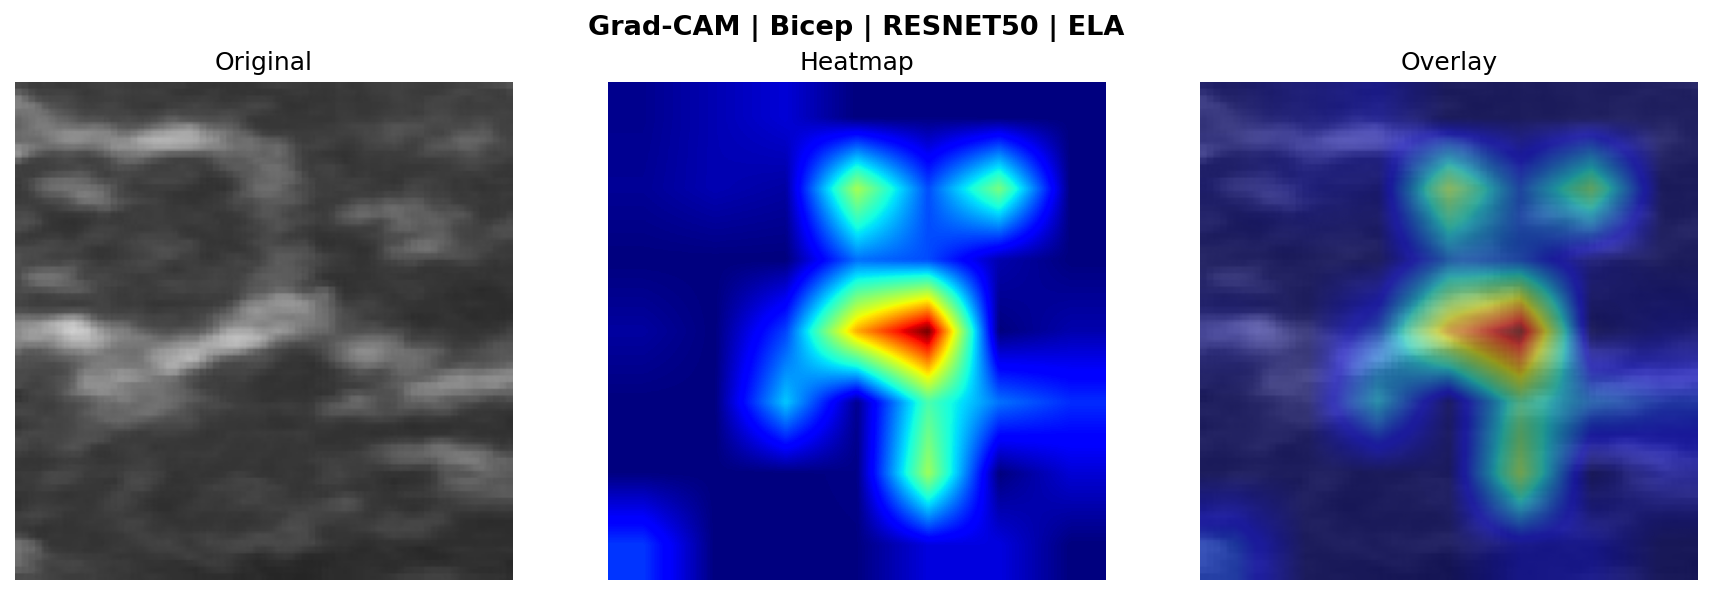
\includegraphics[width=0.22\textwidth]{images/explainability/gradcam/Bicep_resnet50_ELA_1.png} &
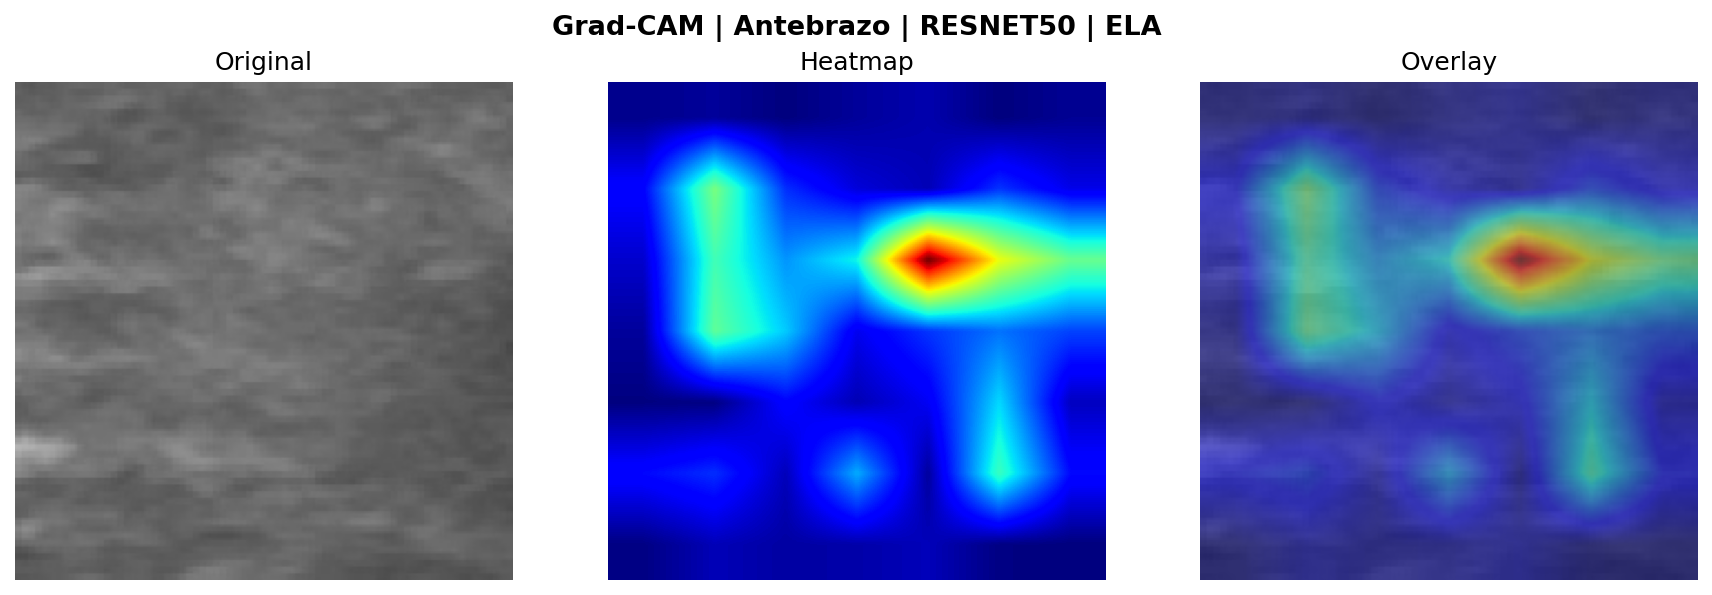
\includegraphics[width=0.22\textwidth]{images/explainability/gradcam/Antebrazo_resnet50_ELA_1.png} &
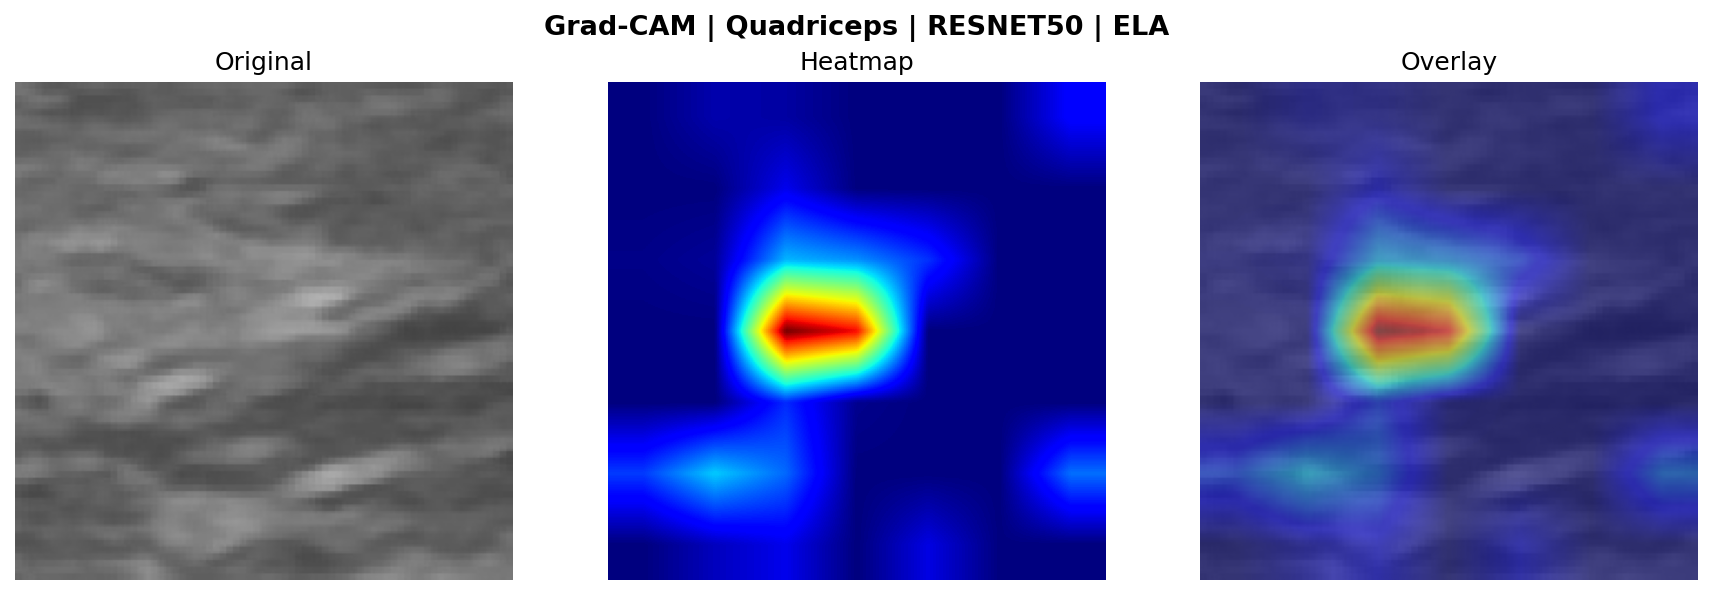
\includegraphics[width=0.22\textwidth]{images/explainability/gradcam/Quadriceps_resnet50_ELA_1.png} &
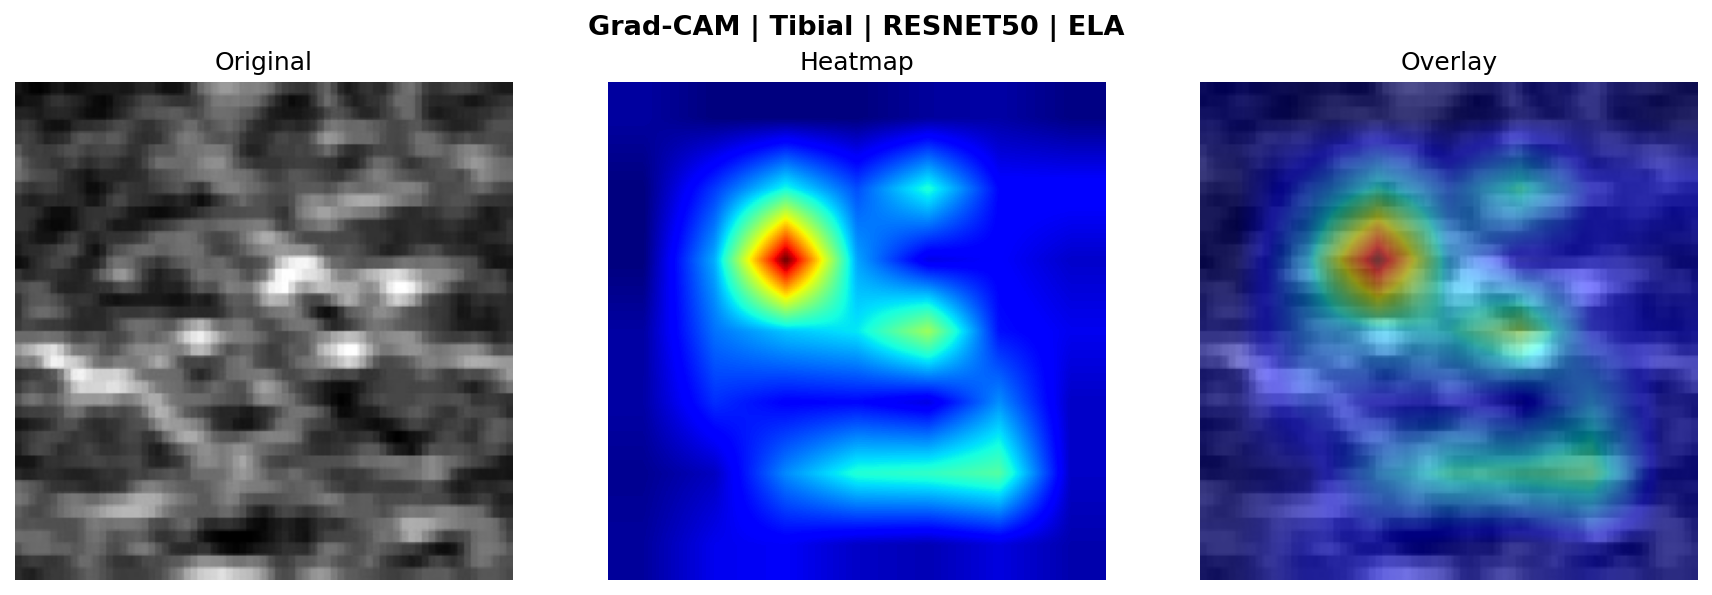
\includegraphics[width=0.22\textwidth]{images/explainability/gradcam/Tibial_resnet50_ELA_1.png} \\
Bíceps & Antebrazo & Cuádriceps & Tibial \\
\end{tabular}
\caption{Grad-CAM sobre un paciente con ELA en cada uno de los cuatro músculos.}
\label{fig:anexo-gradcam}
\end{figure}

\begin{figure}[H]
\centering
\begin{tabular}{cccc}

\includegraphics[width=0.22\textwidth]{images/explainability/guided_gradcam/Bicep_resnet50_ELA_1.png} &

\includegraphics[width=0.22\textwidth]{images/explainability/guided_gradcam/Antebrazo_resnet50_ELA_1.png} &

\includegraphics[width=0.22\textwidth]{images/explainability/guided_gradcam/Quadriceps_resnet50_ELA_1.png} &

\includegraphics[width=0.22\textwidth]{images/explainability/guided_gradcam/Tibial_resnet50_ELA_1.png} \\
Bíceps & Antebrazo & Cuádriceps & Tibial \\
\end{tabular}
\caption{Grad-CAM guiado sobre los mismos pacientes con ELA. La técnica combina la localización de Grad-CAM con la retropropagación guiada para refinar la atribución a píxeles concretos.}
\label{fig:anexo-guided}
\end{figure}

\begin{figure}[H]
\centering
\begin{tabular}{cccc}

\includegraphics[width=0.22\textwidth]{images/explainability/saliency/Bicep_resnet50_ELA_1.png} &

\includegraphics[width=0.22\textwidth]{images/explainability/saliency/Antebrazo_resnet50_ELA_1.png} &

\includegraphics[width=0.22\textwidth]{images/explainability/saliency/Quadriceps_resnet50_ELA_1.png} &

\includegraphics[width=0.22\textwidth]{images/explainability/saliency/Tibial_resnet50_ELA_1.png} \\
Bíceps & Antebrazo & Cuádriceps & Tibial \\
\end{tabular}
\caption{Mapas de saliencia sobre los mismos pacientes. Visualizan el gradiente de la probabilidad de ELA respecto a cada píxel de entrada.}
\label{fig:anexo-saliency}
\end{figure}

\begin{figure}[H]
\centering
\begin{tabular}{cccc}

\includegraphics[width=0.22\textwidth]{images/explainability/occlusion/Bicep_resnet50_ELA_1.png} &

\includegraphics[width=0.22\textwidth]{images/explainability/occlusion/Antebrazo_resnet50_ELA_1.png} &

\includegraphics[width=0.22\textwidth]{images/explainability/occlusion/Quadriceps_resnet50_ELA_1.png} &

\includegraphics[width=0.22\textwidth]{images/explainability/occlusion/Tibial_resnet50_ELA_1.png} \\
Bíceps & Antebrazo & Cuádriceps & Tibial \\
\end{tabular}
\caption{Análisis por oclusión sobre los mismos pacientes. Cuantifica la caída de la probabilidad de ELA al ocultar parches de la imagen, identificando las regiones cuya información es más crítica para la decisión del modelo.}
\label{fig:anexo-occlusion}
\end{figure}

Las cuatro técnicas coinciden cualitativamente: las regiones de mayor influencia se concentran sobre el tejido muscular, no sobre los bordes ni sobre las anotaciones automáticas del ecógrafo. La convergencia de cuatro métodos de explicabilidad mecánicamente distintos sobre los mismos focos refuerza la interpretación: las decisiones del modelo se apoyan en patrones reproducibles y plausibles desde el punto de vista clínico.

\end{document}




